\chapter{Програмни конструкции}

Компютърните програми са съставени от стриктна последователност инструкции. Такива последователности се наричат алгоритъм. Ние хората всеки ден изпълняваме различни алгоритми, като част от нашето ежедневие. Да се приготвим и да отидем на училище е един алгоритъм. Събуждаме се, ставаме, обличаме се, правим си сутрешния тоалет, закусваме, излизаме от вкъщи, придвижваме се до училище. Много ярък пример за алгоритъм са рецептите за готвене. В една рецепта има начални продукти, след това точни инструкции как продуктите са се обработят и смесят, като има ясна представа какъв трябва да бъде крайният резултат. При компютърните програми има основен набор от инструкции, които съставляват изразните средства на съответния програмен език. Чарът на блоковите езици е, че този основен набор от инструкции е представен визуално, под формата на цветни блокчета. Подредбата на цветните блокчета в строго определена последователност води до създаването на малки компютърни програми. 

В случая на Scratch, програмата има ясно определена стартова точка и ясно определена финална точка. При App Inventor подходът е малко по-различен. Там последователността от инструкции, съставляващи писаната програма, се въвежда в малки фрагменти, наречени събития. Събитията възникват при различни действия от страна на потребителя или операционната система. При Scratch говорим за последователно програмиране, а при App Inventor говорим за събитийно програмиране. Основните програмни конструкции в двете програмни среди до голяма степен са идентични, но има и някои съществени разлики. За да можем да пишем ефективни и надеждни програми е важно добре да познаваме изразните средства на програмните среди с които работим. 

\section{Изразни средства в Scratch}

Базовите градивни блокчета в Scratch са организирани в цветни групи (Фиг. \ref{fig020001}). Тази организация помага за по-бързо ориентиране и по-ефективна употреба на различните блокчета. 

\begin{figure}[H]
  \centering
  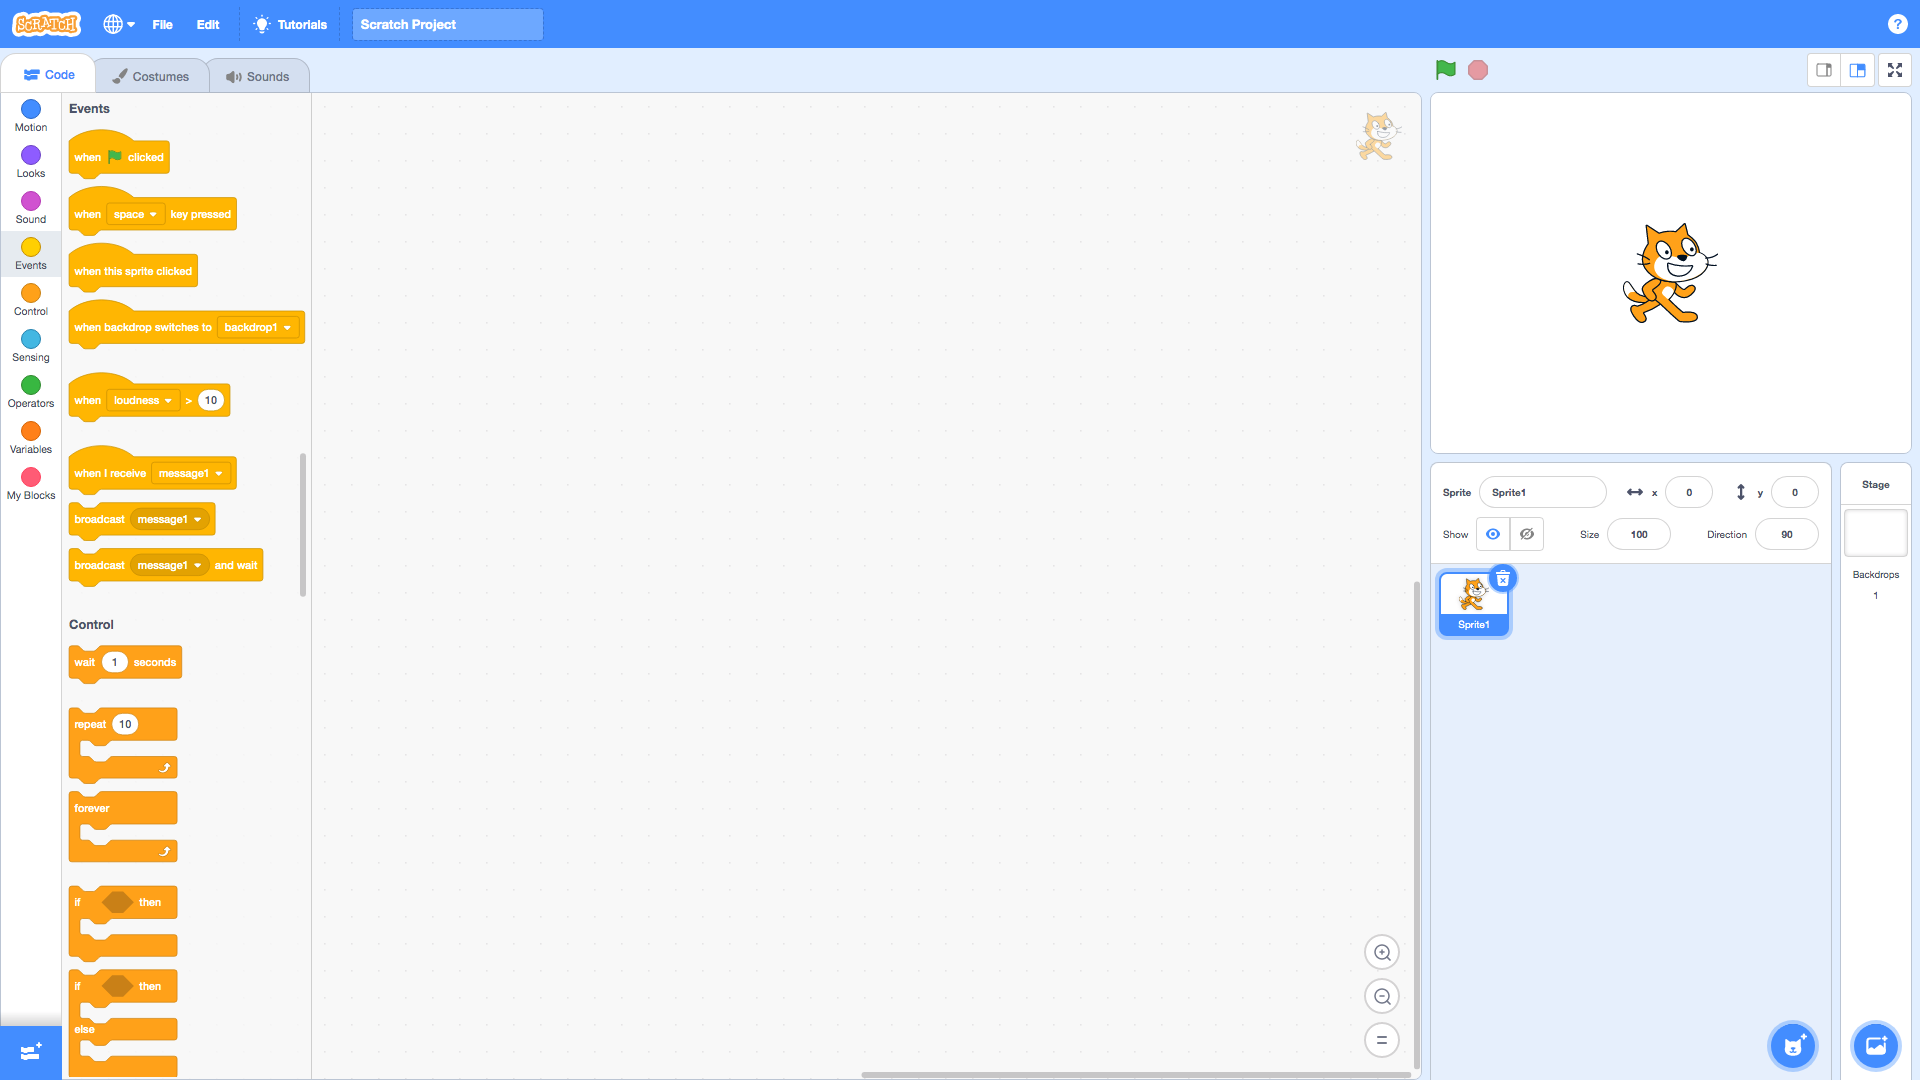
\includegraphics[width=1.0\linewidth,height=0.5\linewidth]{fig020001.png}
  \caption{Групиране на инструкциите}
\label{fig020001}
\end{figure}

Най-важното блокче в програмата е блокчето, което дава старт за изпълнение на инструкциите, които са подредени под него. Това блокче има зелен флаг (Фиг. \ref{fig020002}) и определя какво ще последва след стартирането на програмата.

\begin{figure}[H]
  \centering
  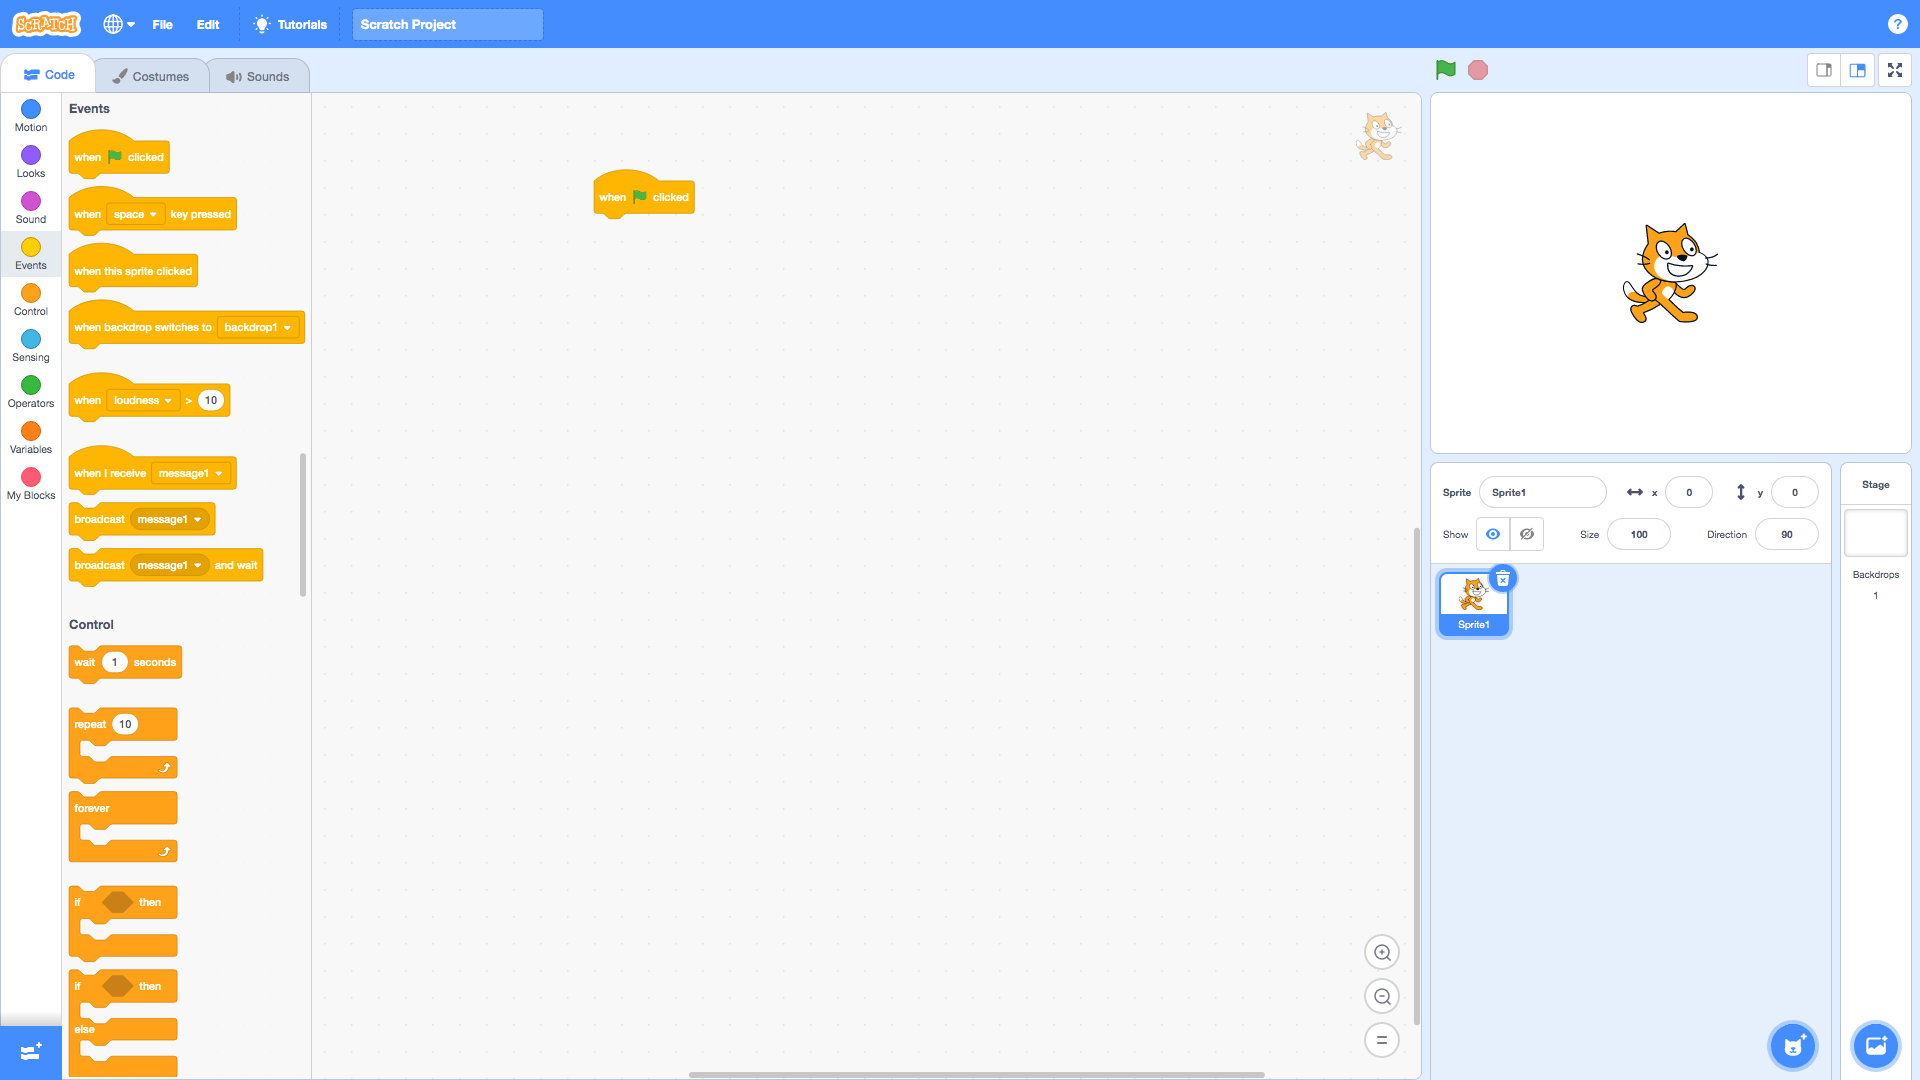
\includegraphics[width=1.0\linewidth,height=0.5\linewidth]{fig020002.png}
  \caption{Начална точка на програмата}
\label{fig020002}
\end{figure}

Блокчето за старт на програмата се намира в светло оранжевата група, която е предназначена да реагира на събития от страна на потребителя. Точният момент в който потребителят иска програмата да започне своето изпълнение е неопределен във времето и поради тази причина Scratch трябва да улови събитие, предизвикано от самия потребител. 

Второто по важност блокче служи за край на програмата (Фиг. \ref{fig020003}). То се намира в тъмно оранжевата група и има за задача да спре всички процеси, извършващи се по време на изпълнението на самата програма.

\begin{figure}[H]
  \centering
  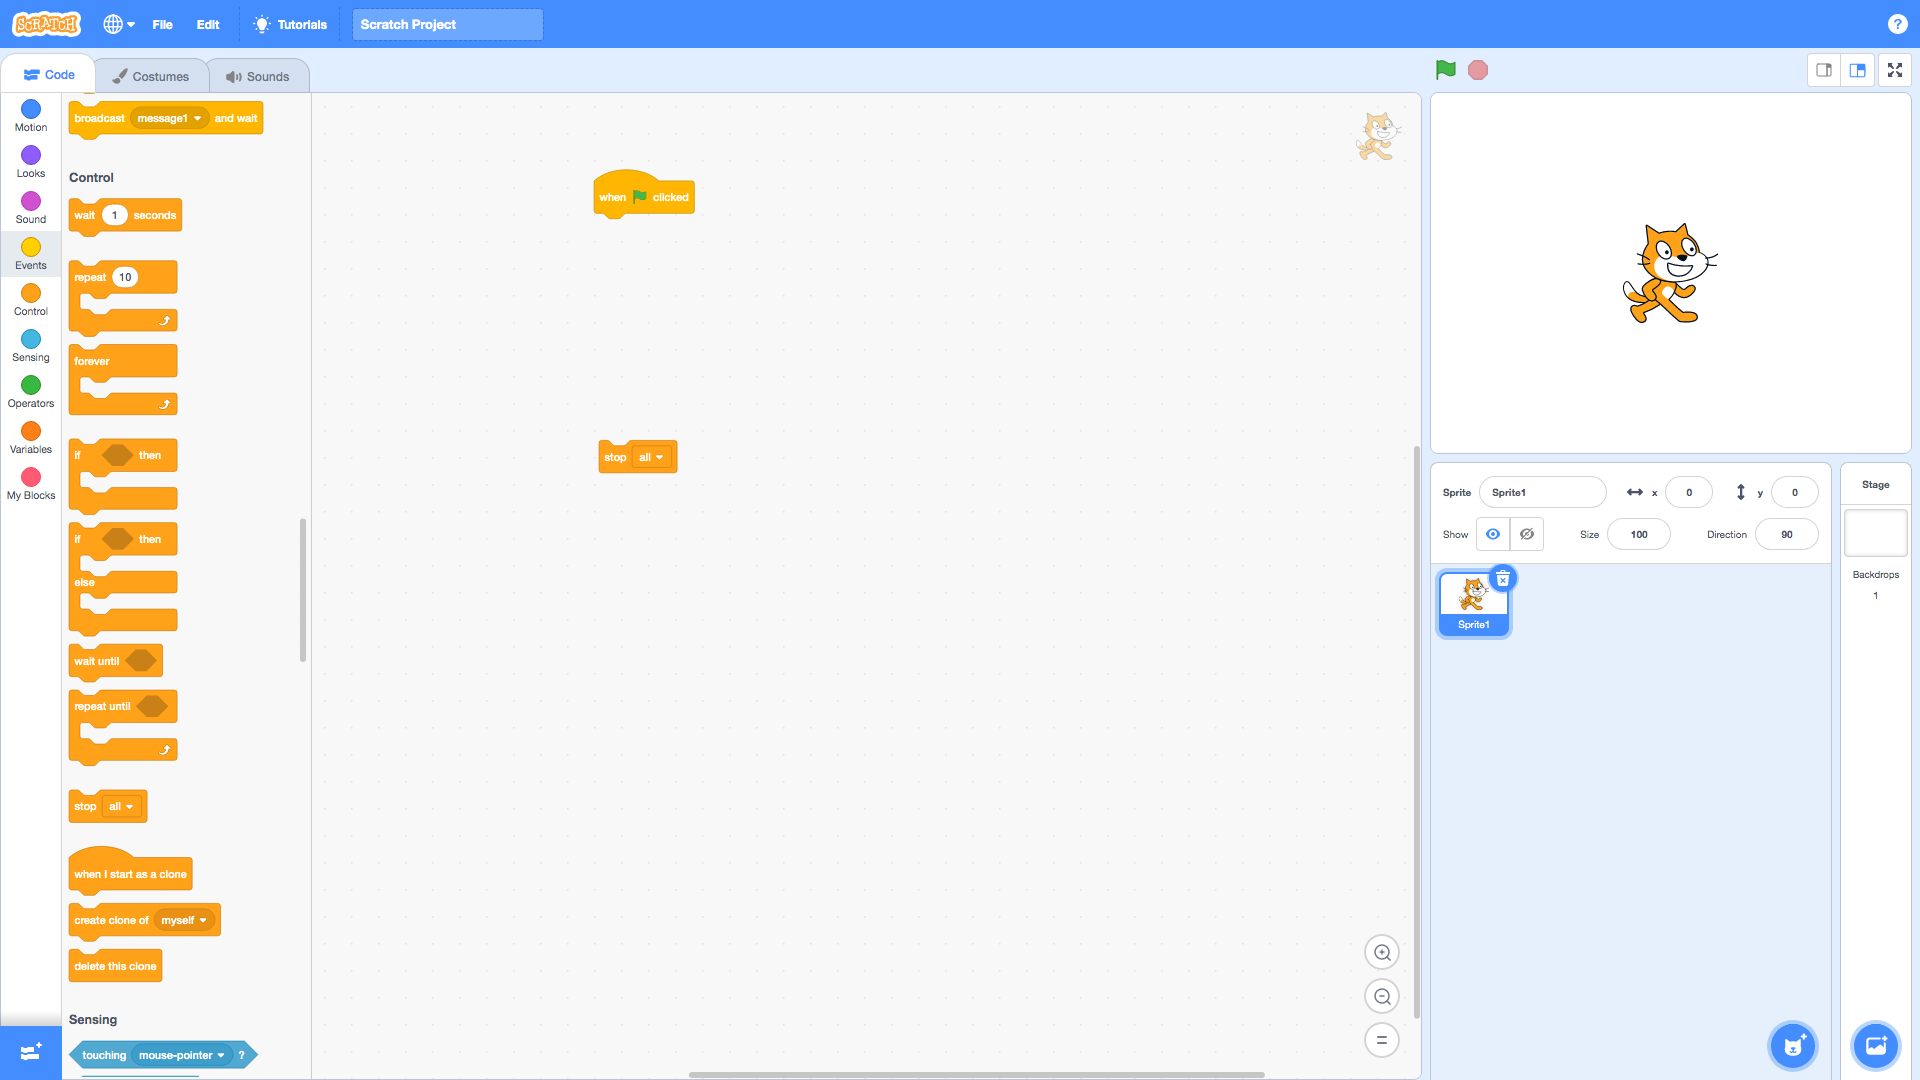
\includegraphics[width=1.0\linewidth,height=0.5\linewidth]{fig020003.png}
  \caption{Крайна точка на програмата}
\label{fig020003}
\end{figure}

Тъмно оранжевата група съдържа блокчета за контрол на изпълнението. Тези блокчета позволяват програмата да поема по различни пътища, както и група от действия да се повтарят многократно. 

В Scratch блокчетата инструкции основно контролират картинки, наречени спрайтове (sprites). За разлика от обикновеното компютърно изображение, спрайтът е графичен обект, който съдържа множество кадри, показващи изображението на героя в различни конфигурации. Всяка нова програма в Scratch започва с един спрайт, на оранжевата котка, разположена на координати (x=0,y=0). Работното пространство е двуизмерна координатна система с център (0,0). 

\begin{figure}[H]
  \centering
  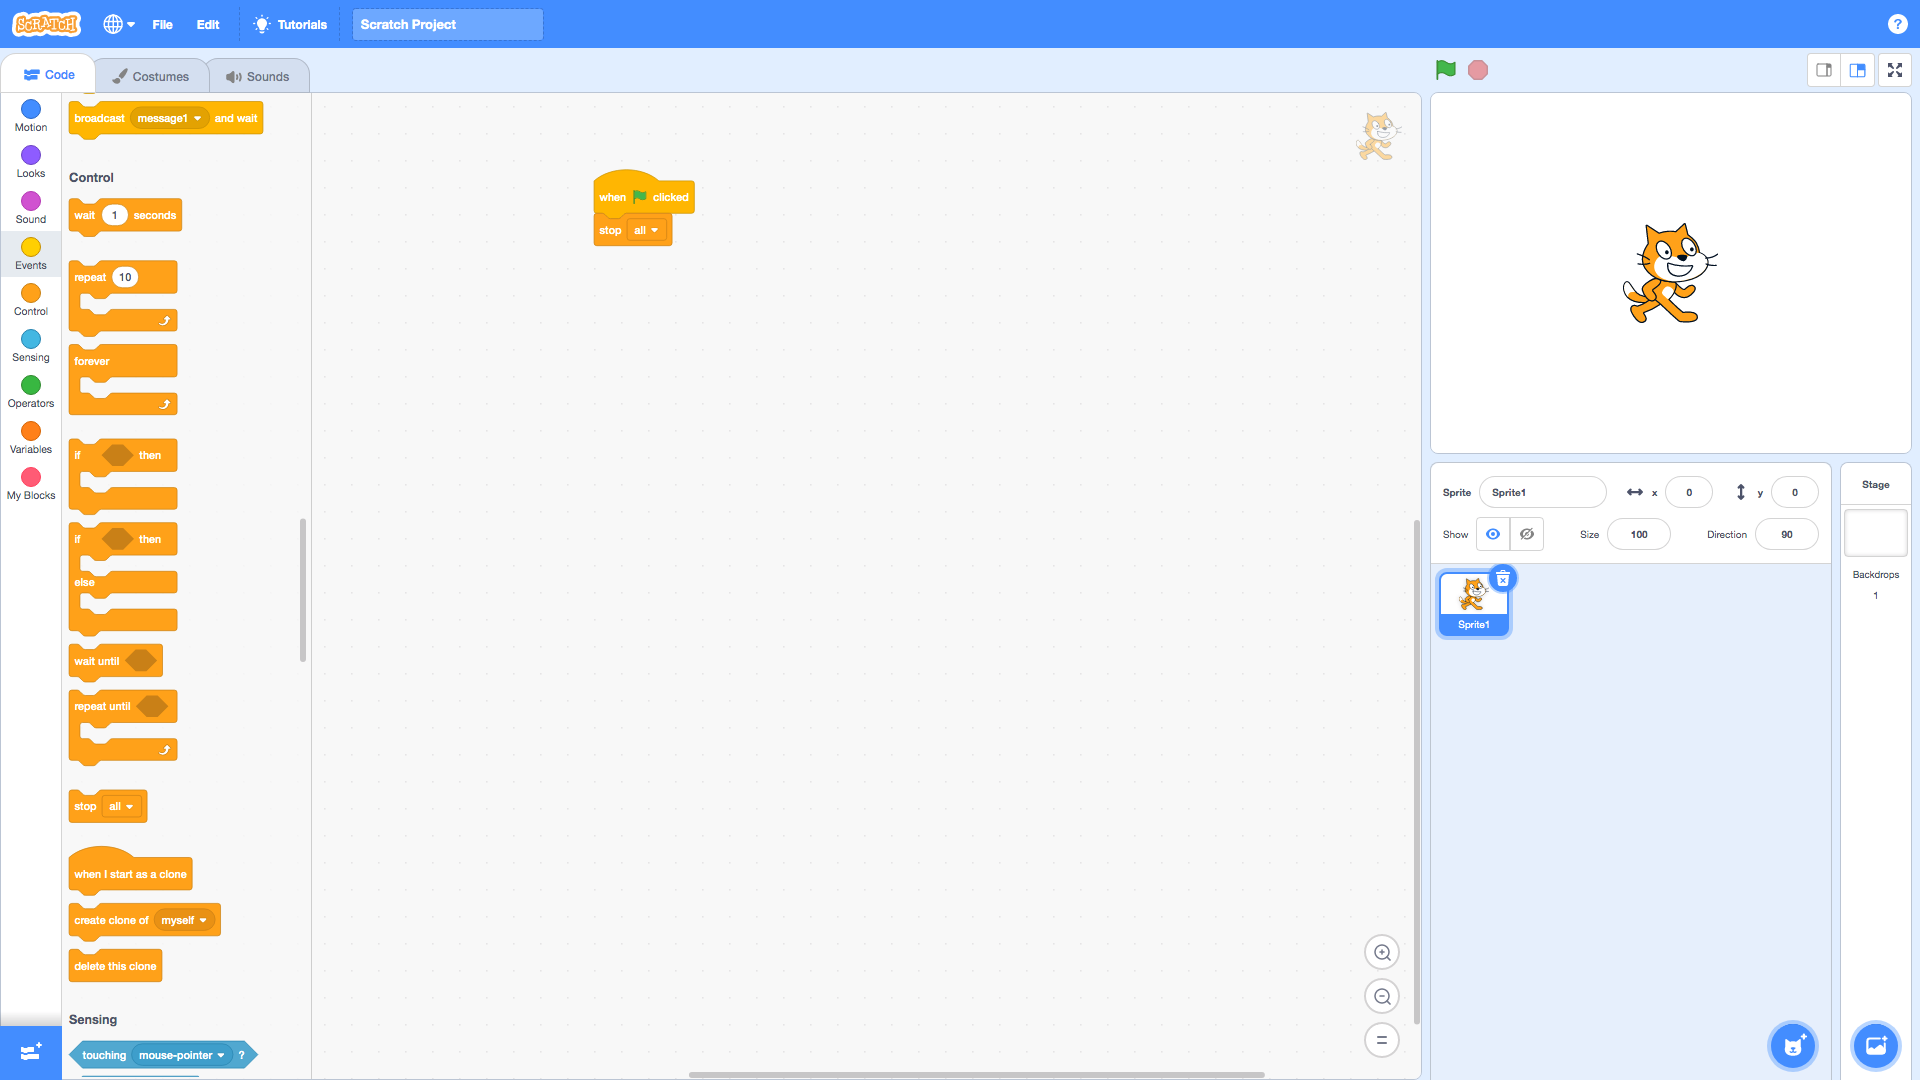
\includegraphics[width=1.0\linewidth,height=0.5\linewidth]{fig020004.png}
  \caption{Завършване веднага след започване}
\label{fig020004}
\end{figure}

Ако бъдат съединени, блокчетата за начало и за край (Фиг. \ref{fig020004}), то програмата не изпълнява нищо. Практически, тази програма приключва веднага след като е започнала. Програма, която не прави нищо е напълно безсмислена. За да започне нещо да се случва се използват блокчетата в синята група. Първото блокче инструктира котето да се премести 10 стъпки, като броя стъпки може да бъде променени, чрез изписване на друго число във вътрешността на блокчето (Фиг. \ref{fig020005}).

\begin{figure}[H]
  \centering
  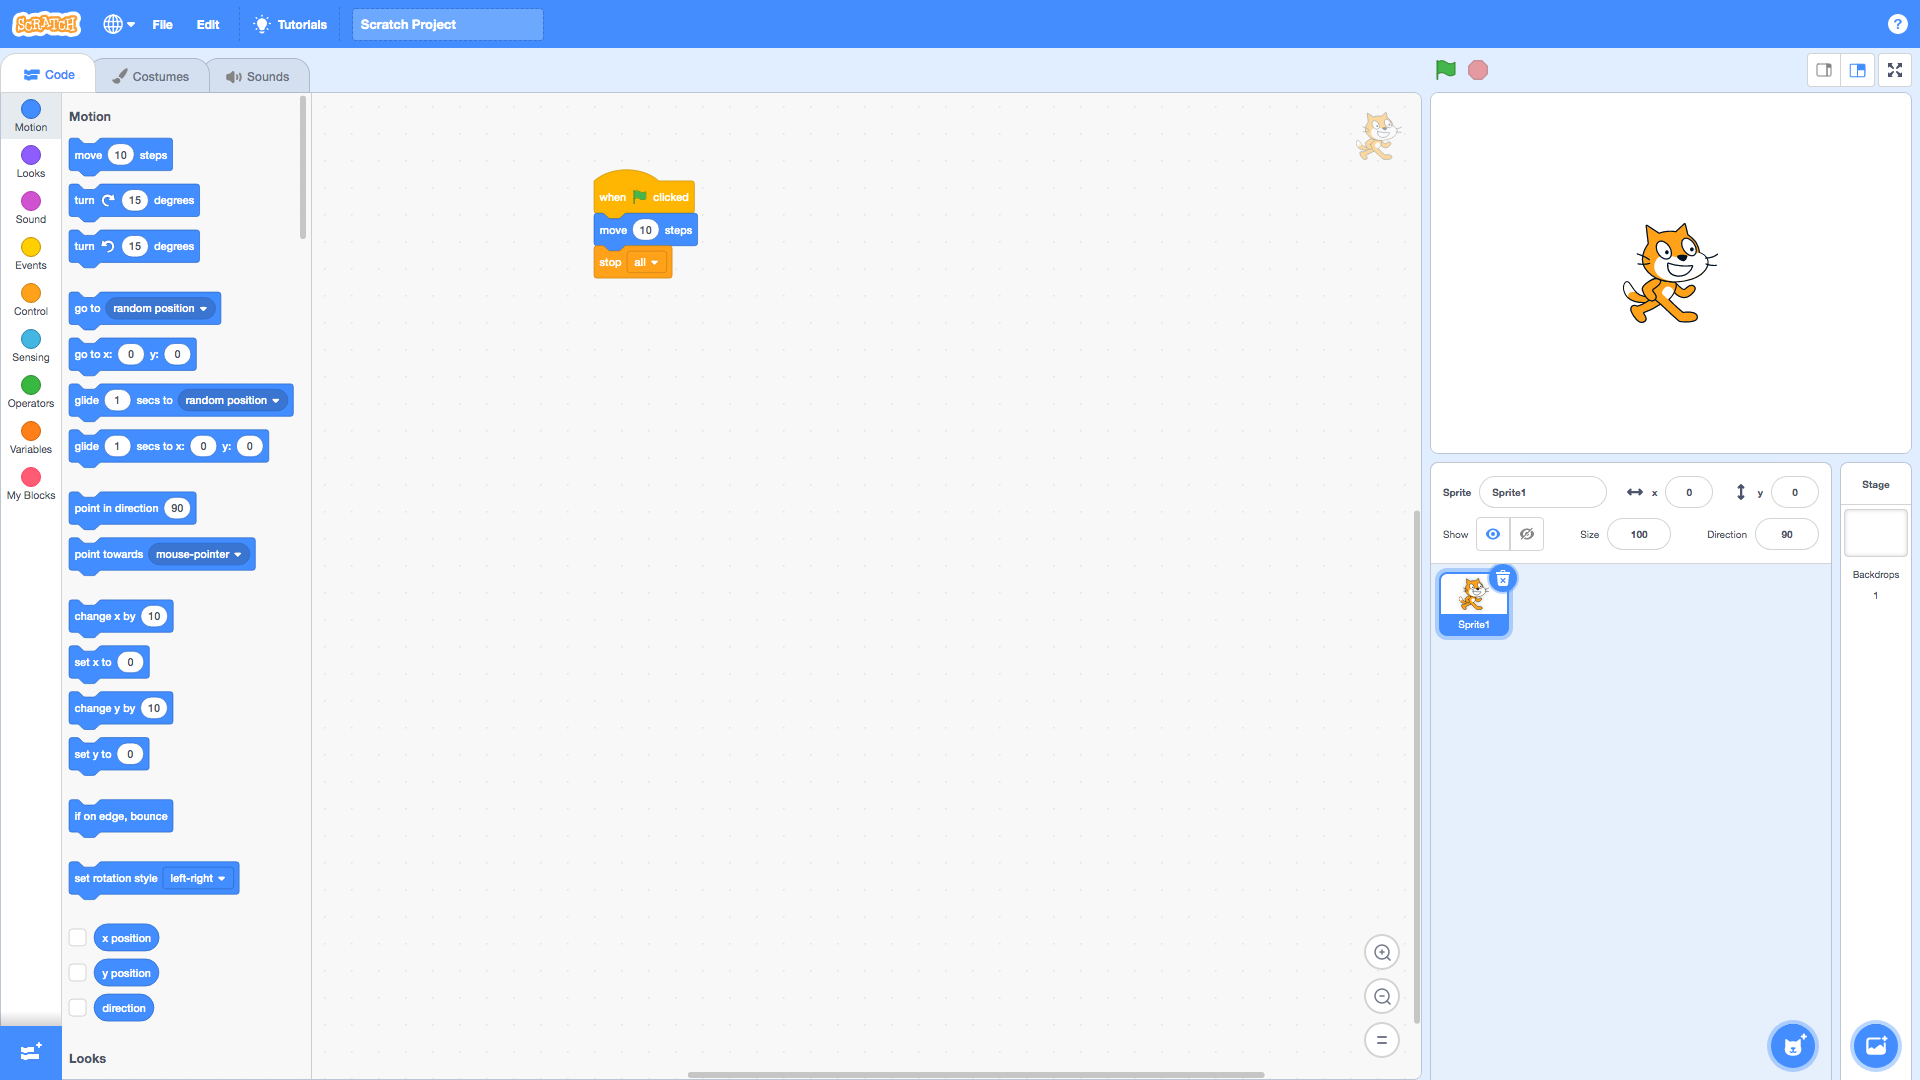
\includegraphics[width=1.0\linewidth,height=0.5\linewidth]{fig020005.png}
  \caption{Преместване на героя}
\label{fig020005}
\end{figure}

Следващият блок в групата инструктира героя да се завърти на определено число градуси, по часовниковата стрелка, спрямо собствения си център (Фиг. \ref{fig020006}).

\begin{figure}[H]
  \centering
  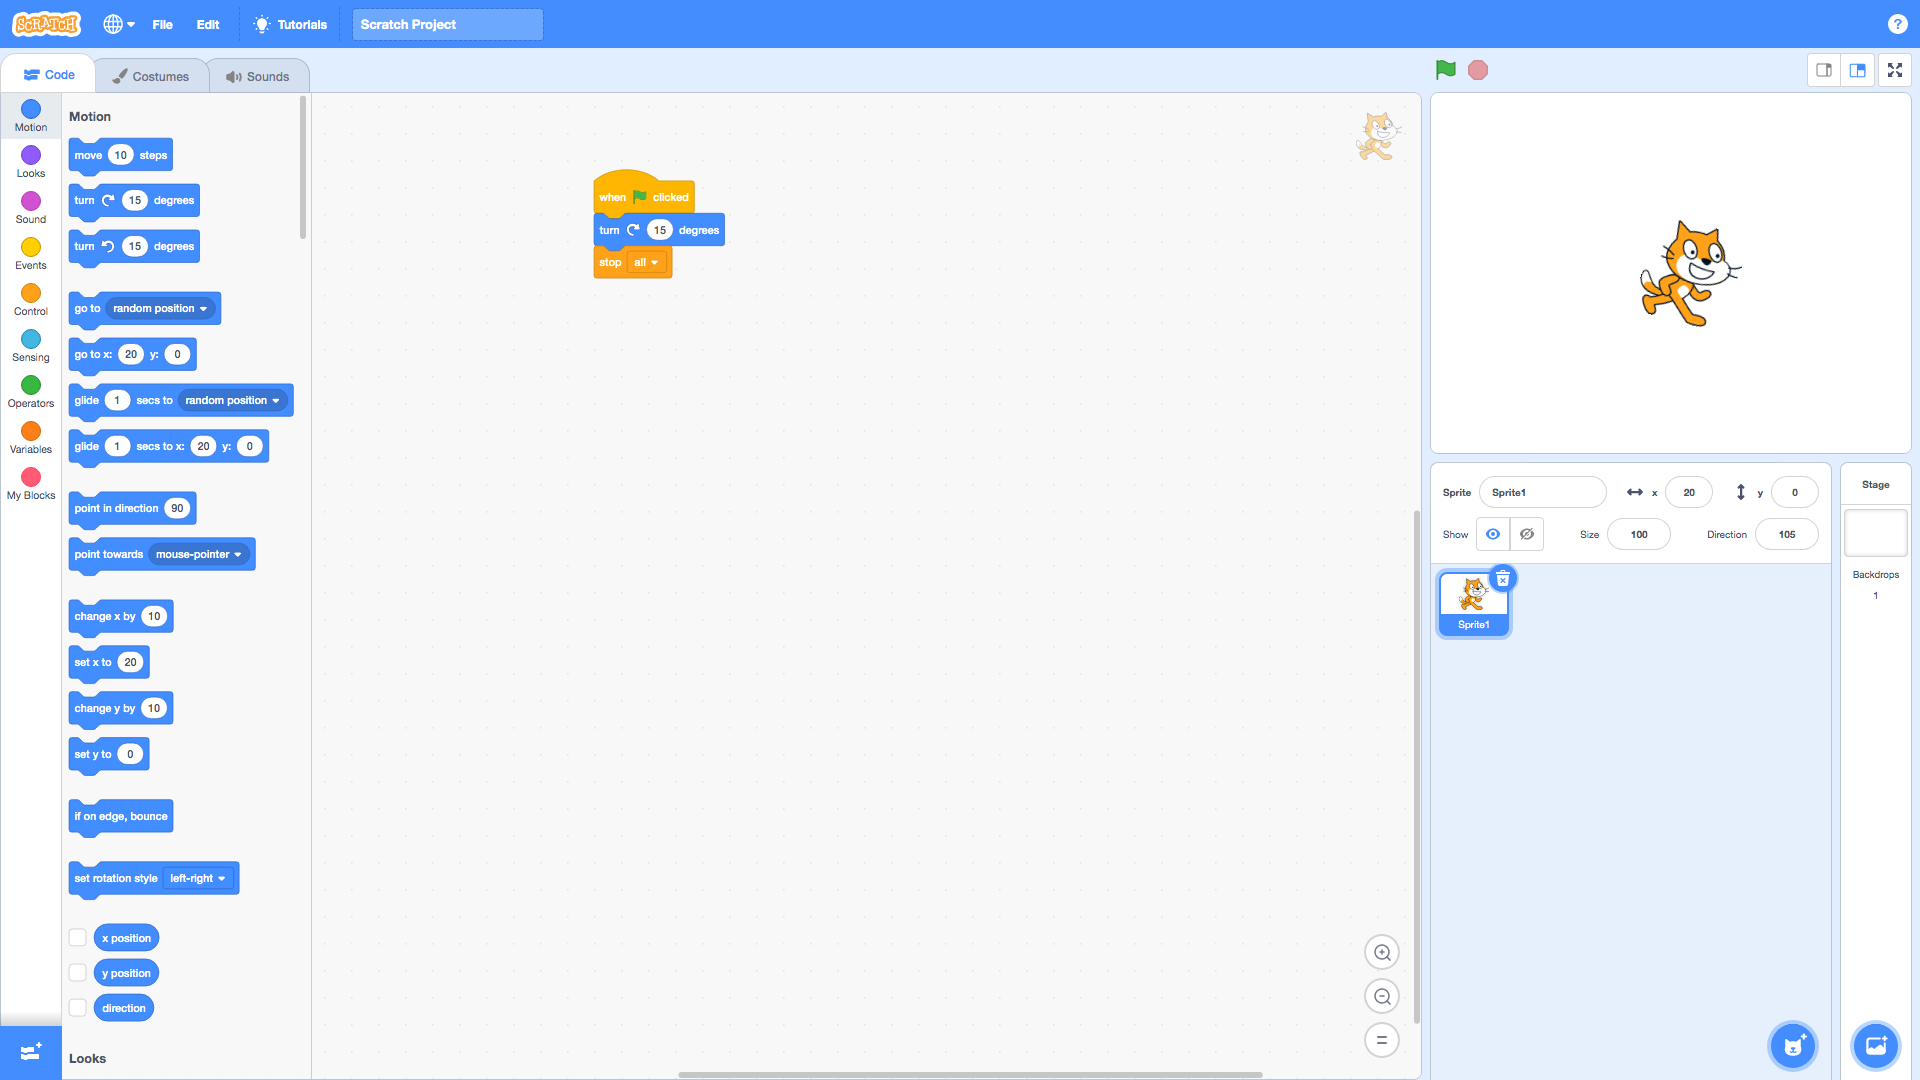
\includegraphics[width=1.0\linewidth,height=0.5\linewidth]{fig020006.png}
  \caption{Завъртане по часовниковата стрелка}
\label{fig020006}
\end{figure}

Аналогично, със следващото блокче в групата, завъртането може да се изпълни и в посока обратна на часовниковата стрелка (Фиг. \ref{fig020007}).

\begin{figure}[H]
  \centering
  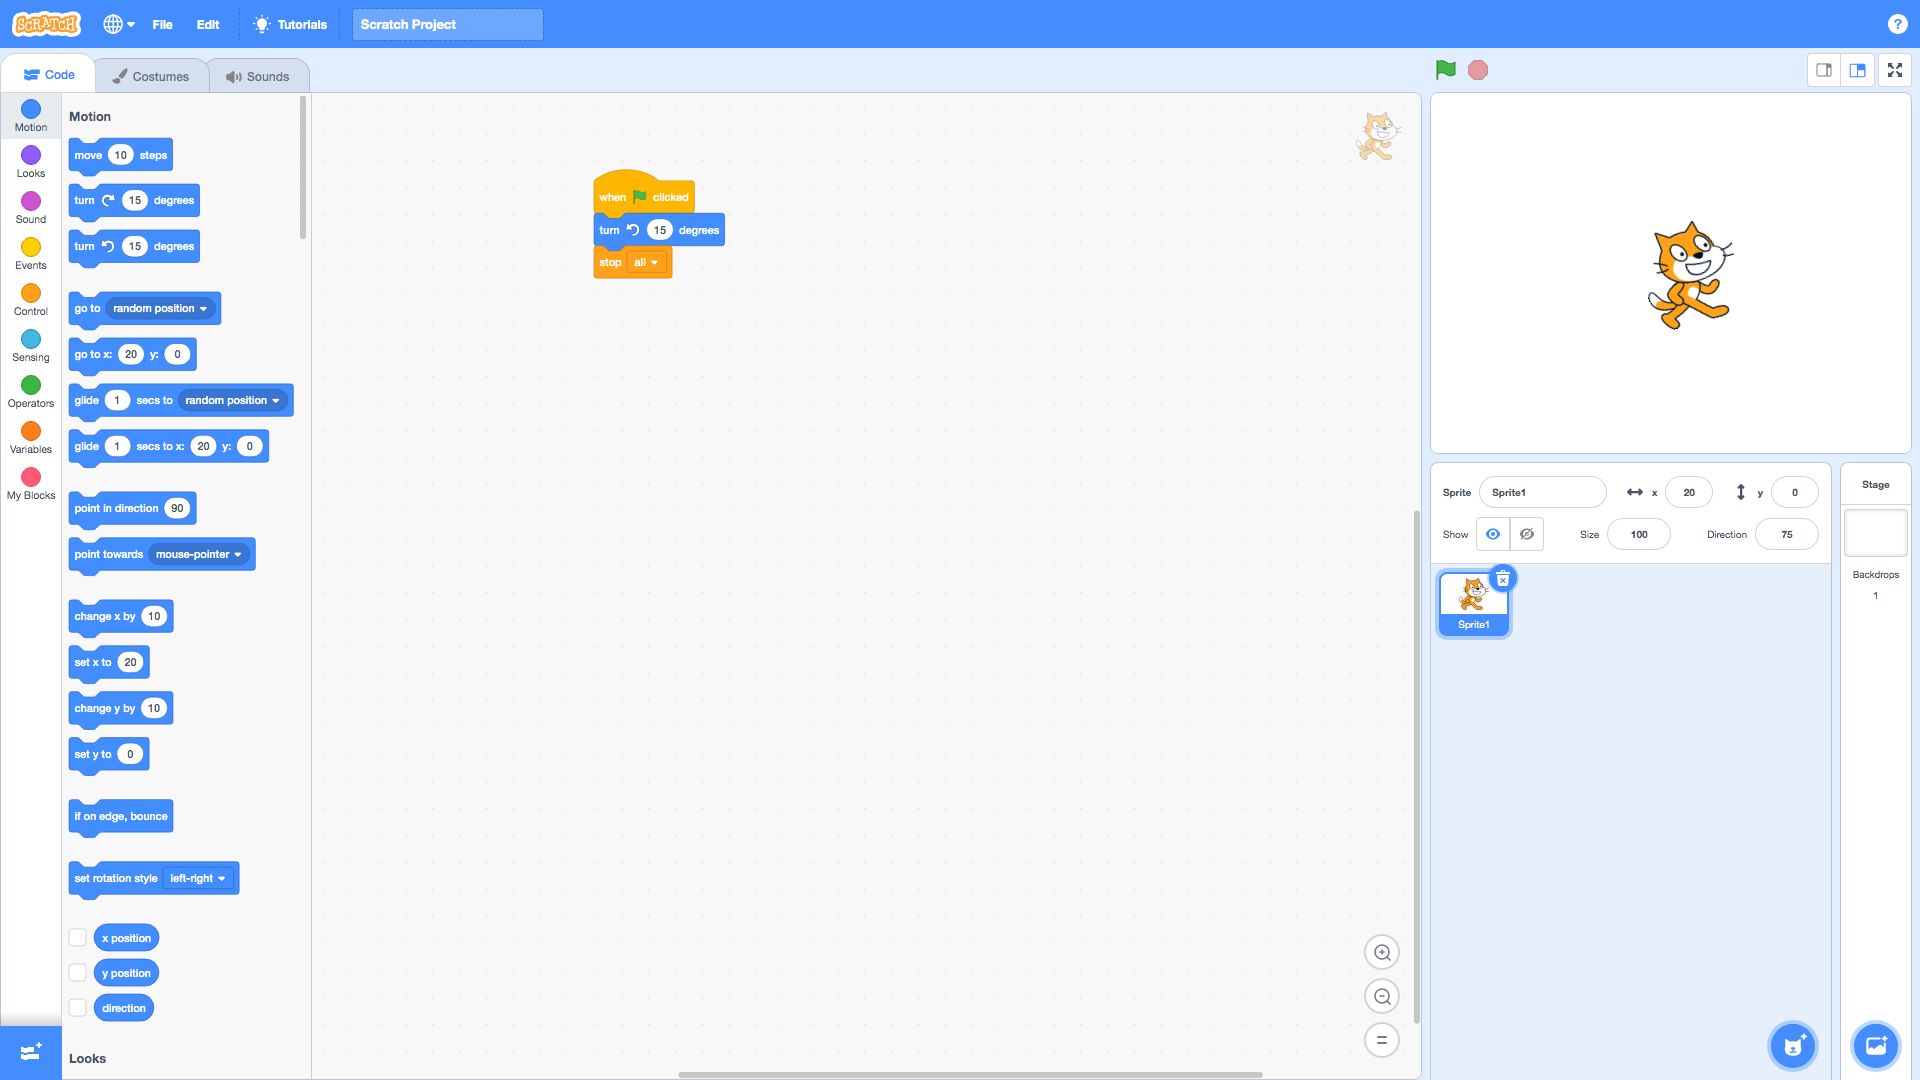
\includegraphics[width=1.0\linewidth,height=0.5\linewidth]{fig020007.png}
  \caption{Завъртане обратно на часовниковата стрелка}
\label{fig020007}
\end{figure}

Следващия блок в групата дава възможност героят да се премести на случайни координати или на координати посочени с мишката (Фиг. \ref{fig020008}).

\begin{figure}[H]
  \centering
  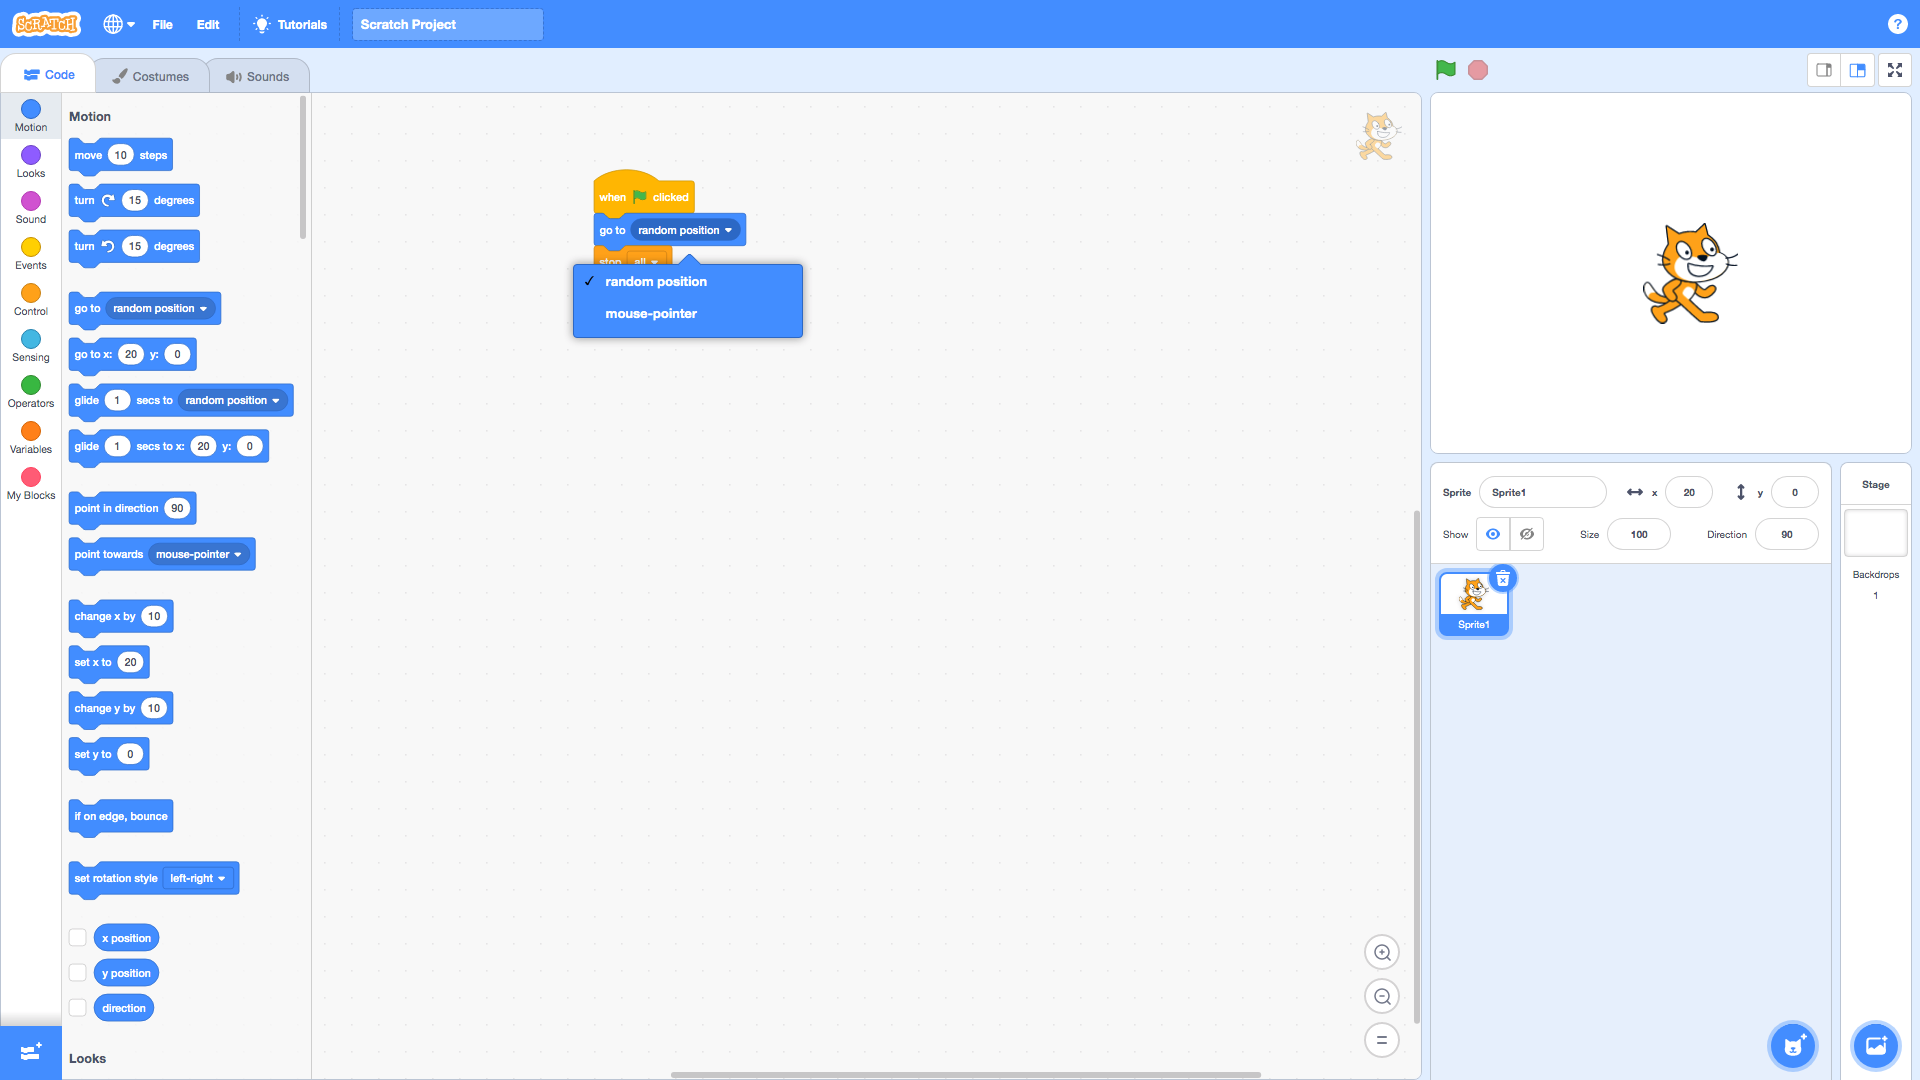
\includegraphics[width=1.0\linewidth,height=0.5\linewidth]{fig020008.png}
  \caption{Преместване на случайна позиция}
\label{fig020008}
\end{figure}

Движението на героя може да бъде зададено и чрез абсолютни координати с блокче, позволяващо да се впишат числа за абцисната и ординатната ос (Фиг. \ref{fig020009}).

\begin{figure}[H]
  \centering
  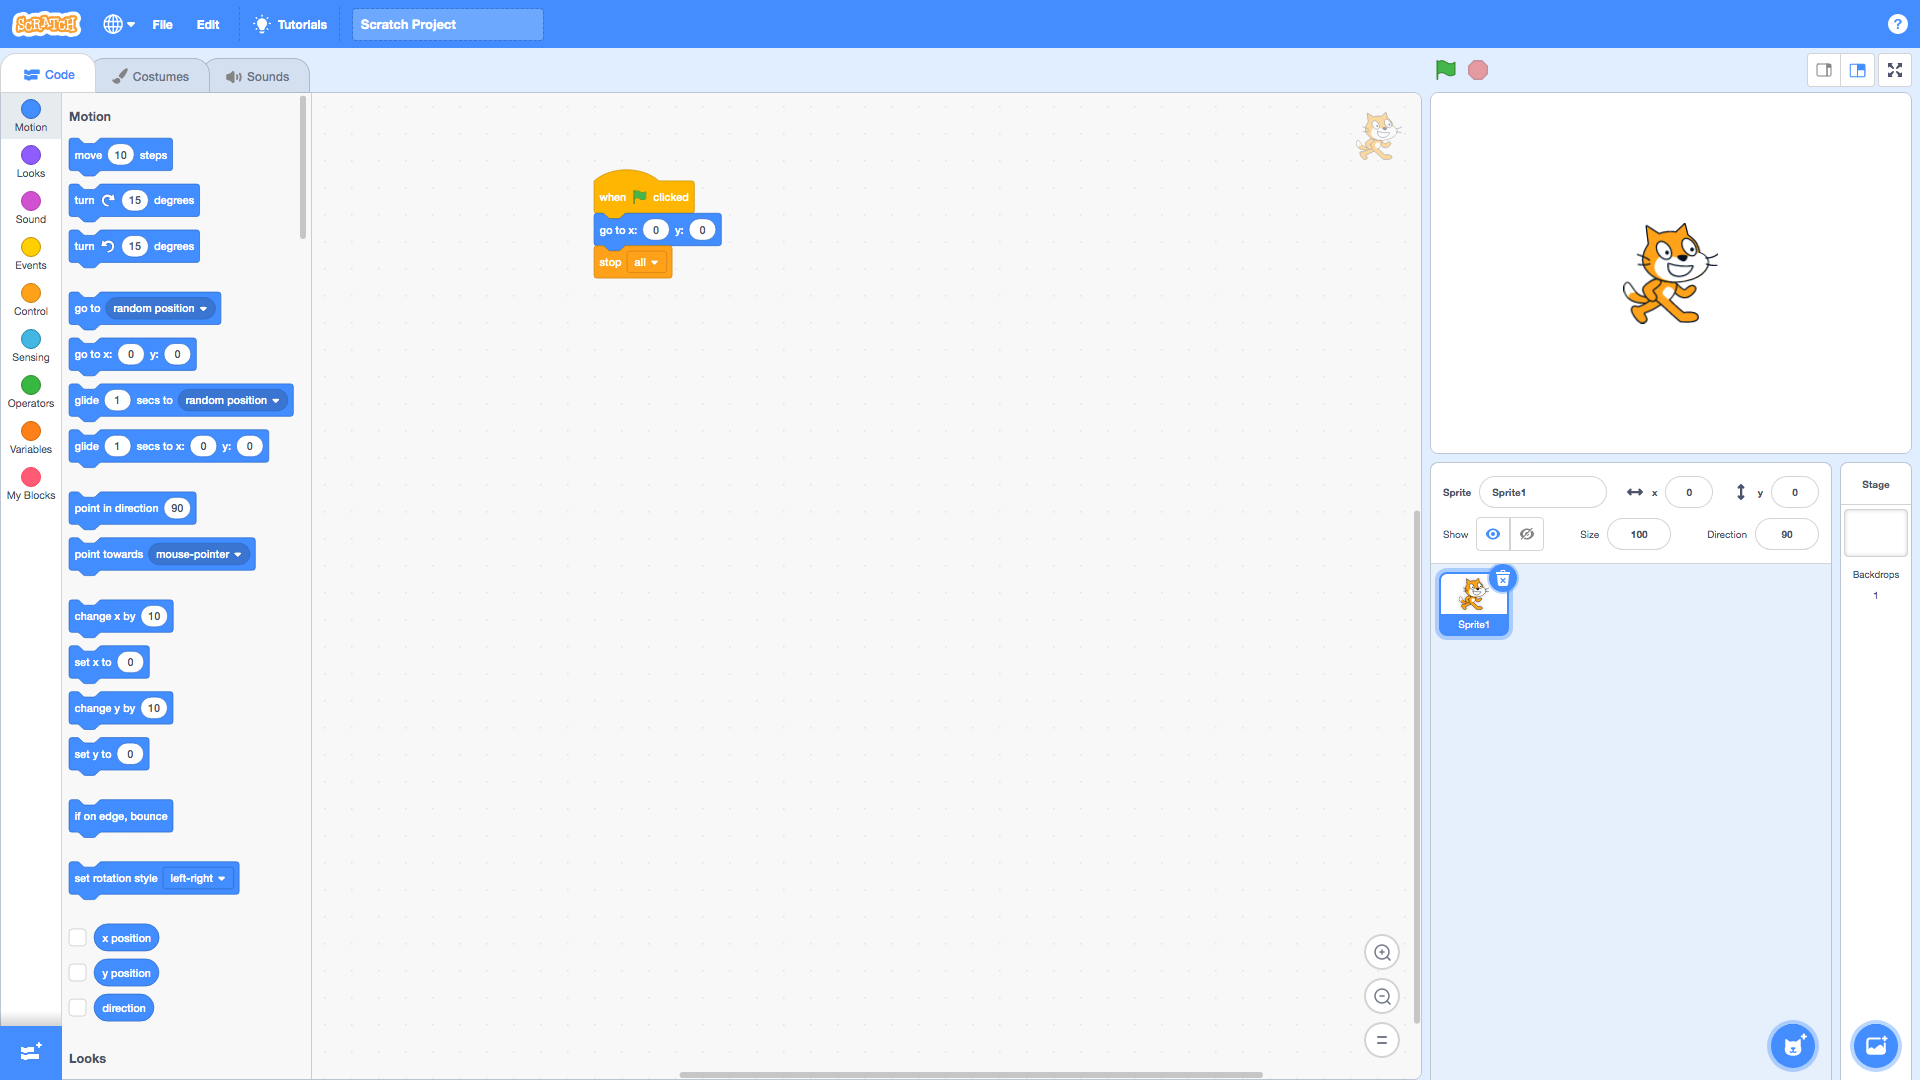
\includegraphics[width=1.0\linewidth,height=0.5\linewidth]{fig020009.png}
  \caption{Преместване по абсолютни координати}
\label{fig020009}
\end{figure}

Плавно придвижване, по предварително зададен интервал от време, е възможно на случайни координати или координати посочени с мишката, благодарение на следващото блокче в групата (Фиг. \ref{fig020010}).

\begin{figure}[H]
  \centering
  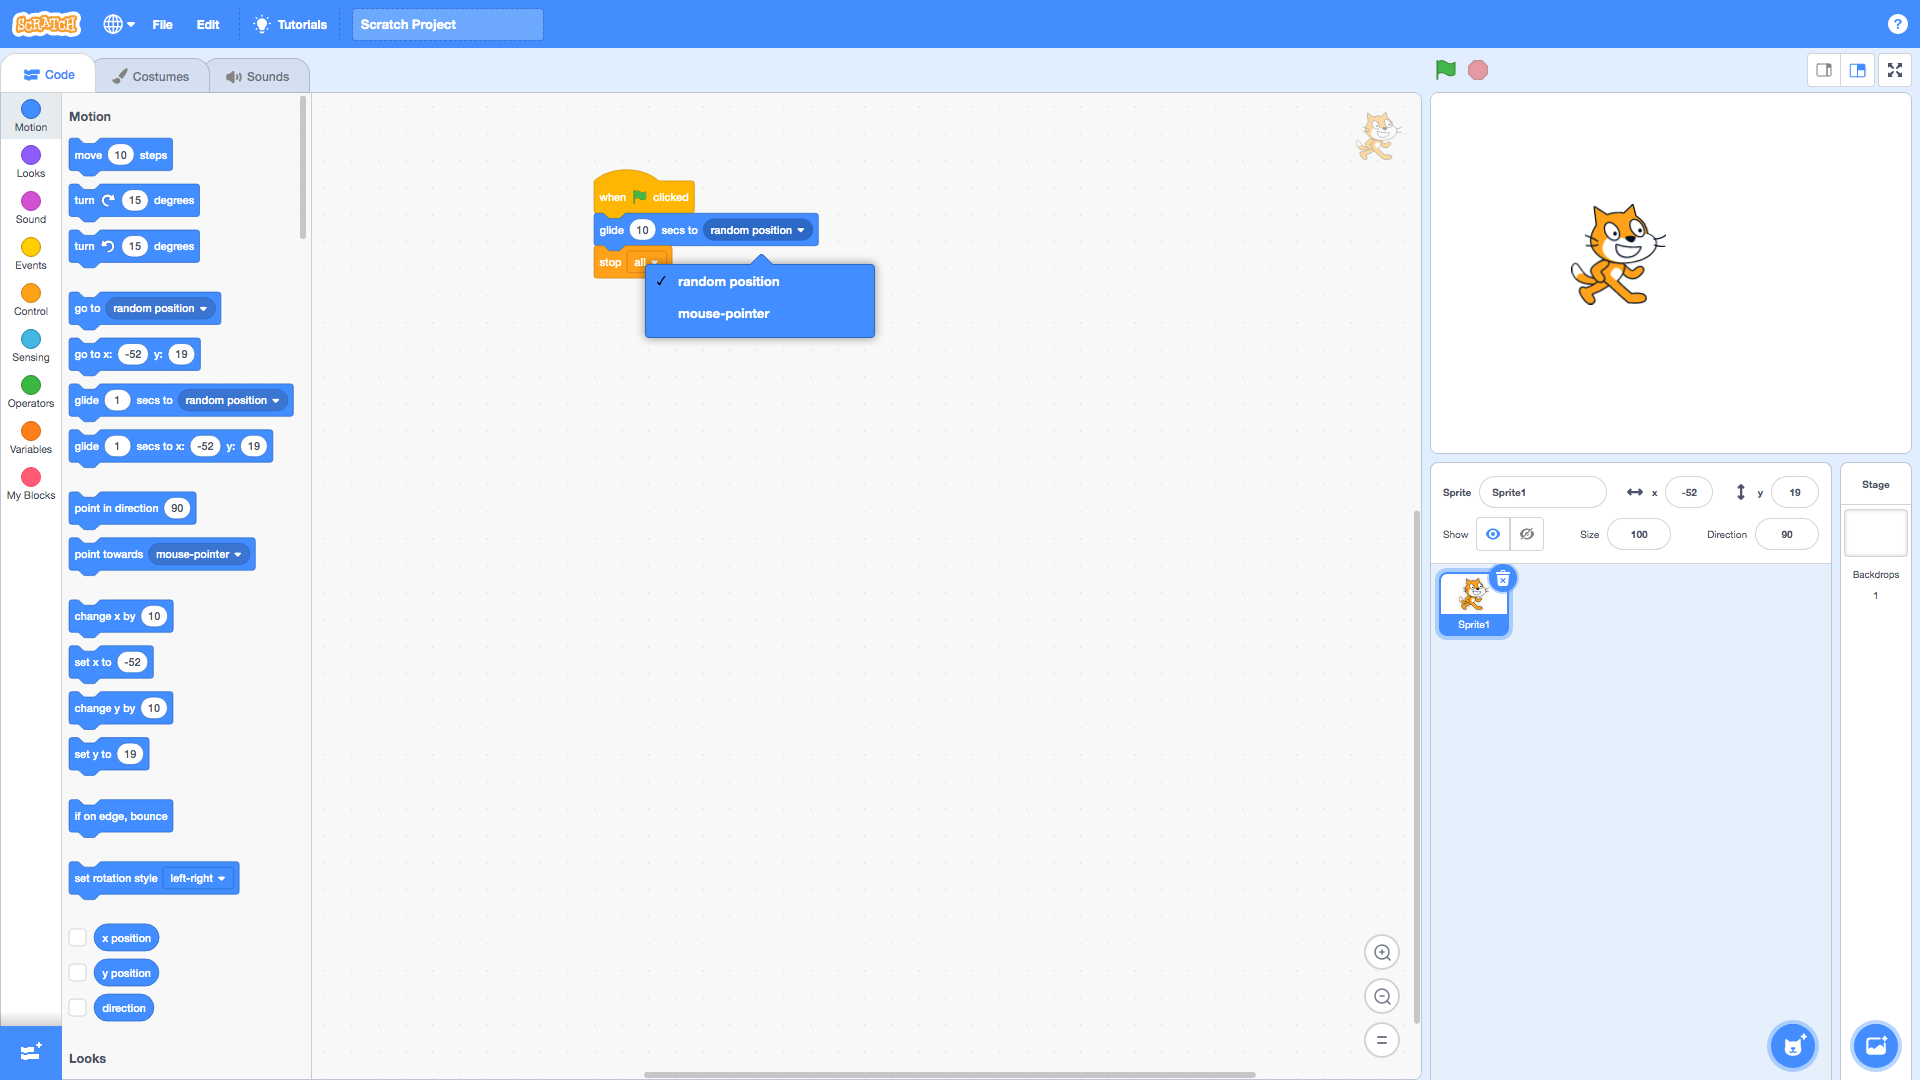
\includegraphics[width=1.0\linewidth,height=0.5\linewidth]{fig020010.png}
  \caption{Плъзгане до случайна позиция}
\label{fig020010}
\end{figure}

Плавното плъзгане до предварително зададени координати, за предварително определен интервал от време, е възможно с блокчето предназначено за тази цел (Фиг. \ref{fig020011}).

\begin{figure}[H]
  \centering
  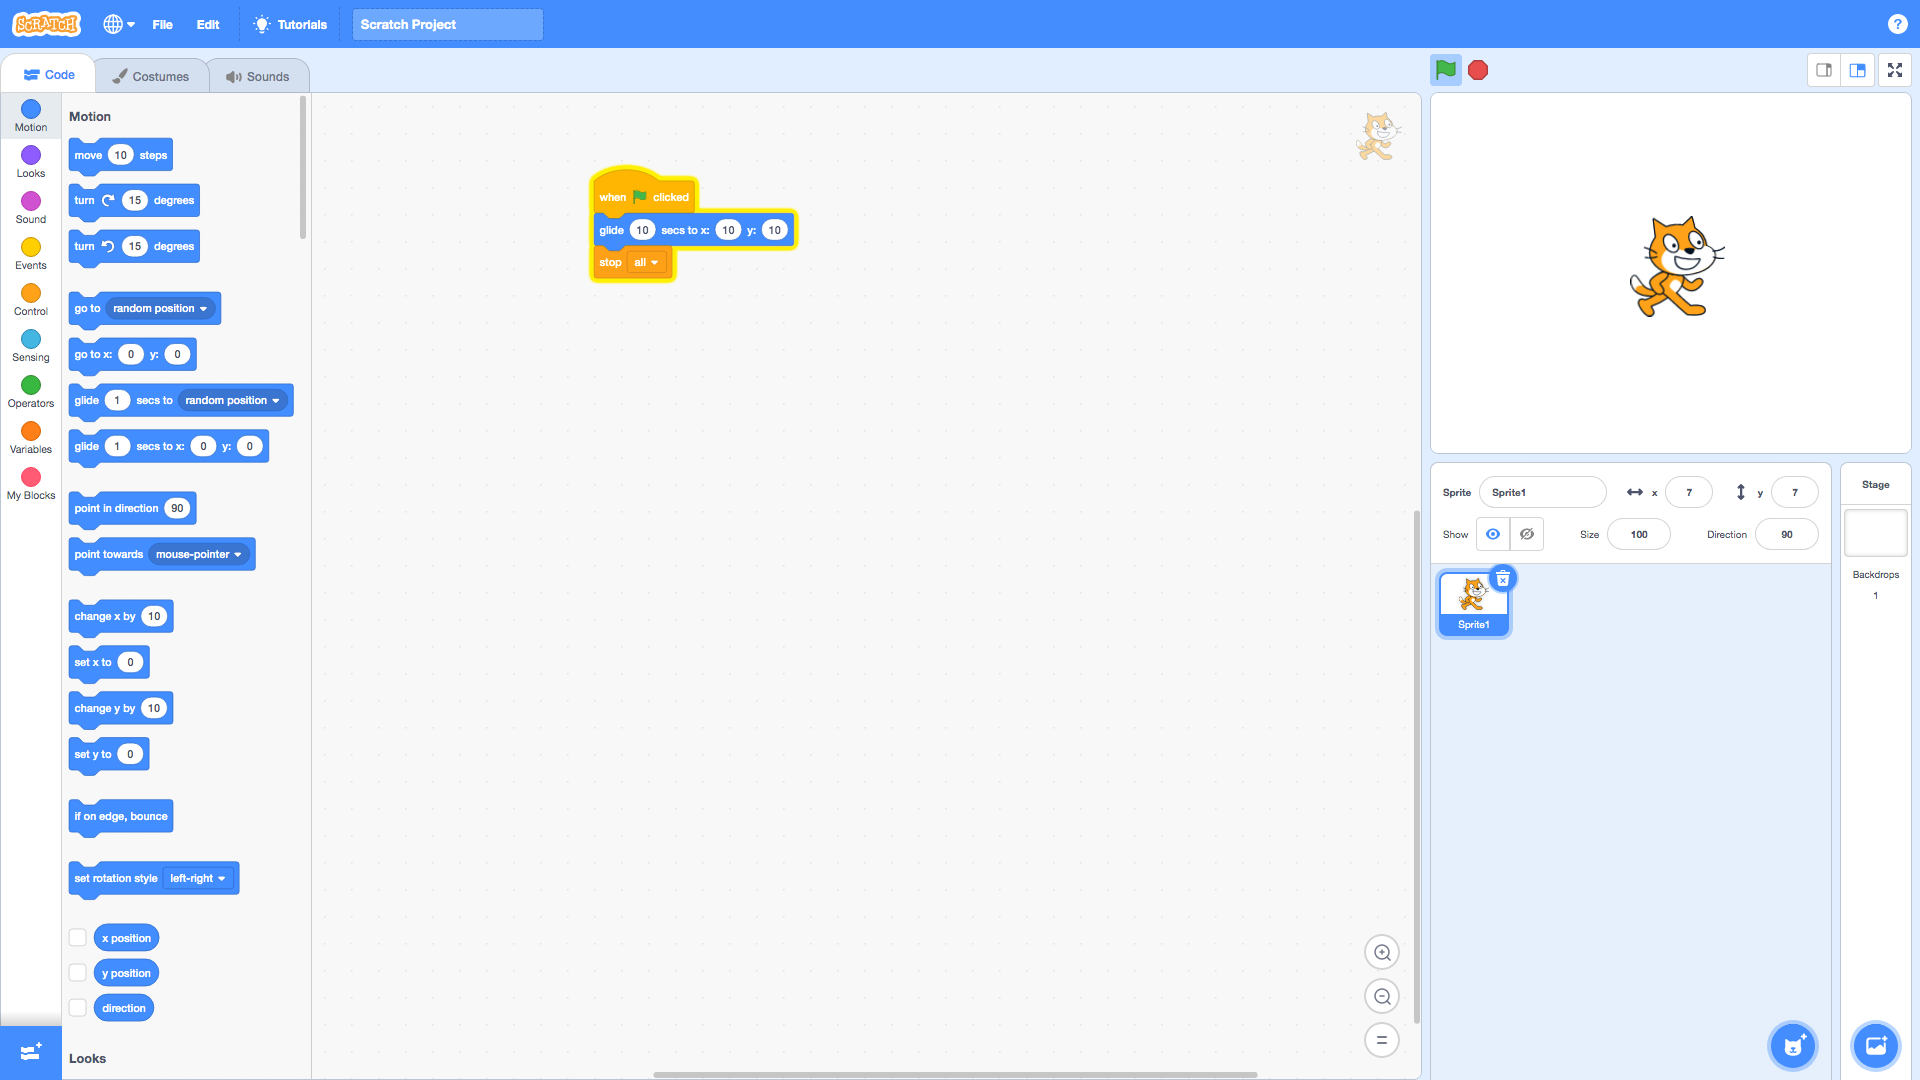
\includegraphics[width=1.0\linewidth,height=0.5\linewidth]{fig020011.png}
  \caption{Плъзгане до зададени координати}
\label{fig020011}
\end{figure}

Анимираният герой има характеристика за ориентация, под формата на ъгъл. При 90 градуса, оранжевата котка гледа на дясно. За да се промени ориентацията на героя се използва блокче с възможност за въвеждане на конкретен ъгъл (Фиг. \ref{fig020012}).

\begin{figure}[H]
  \centering
  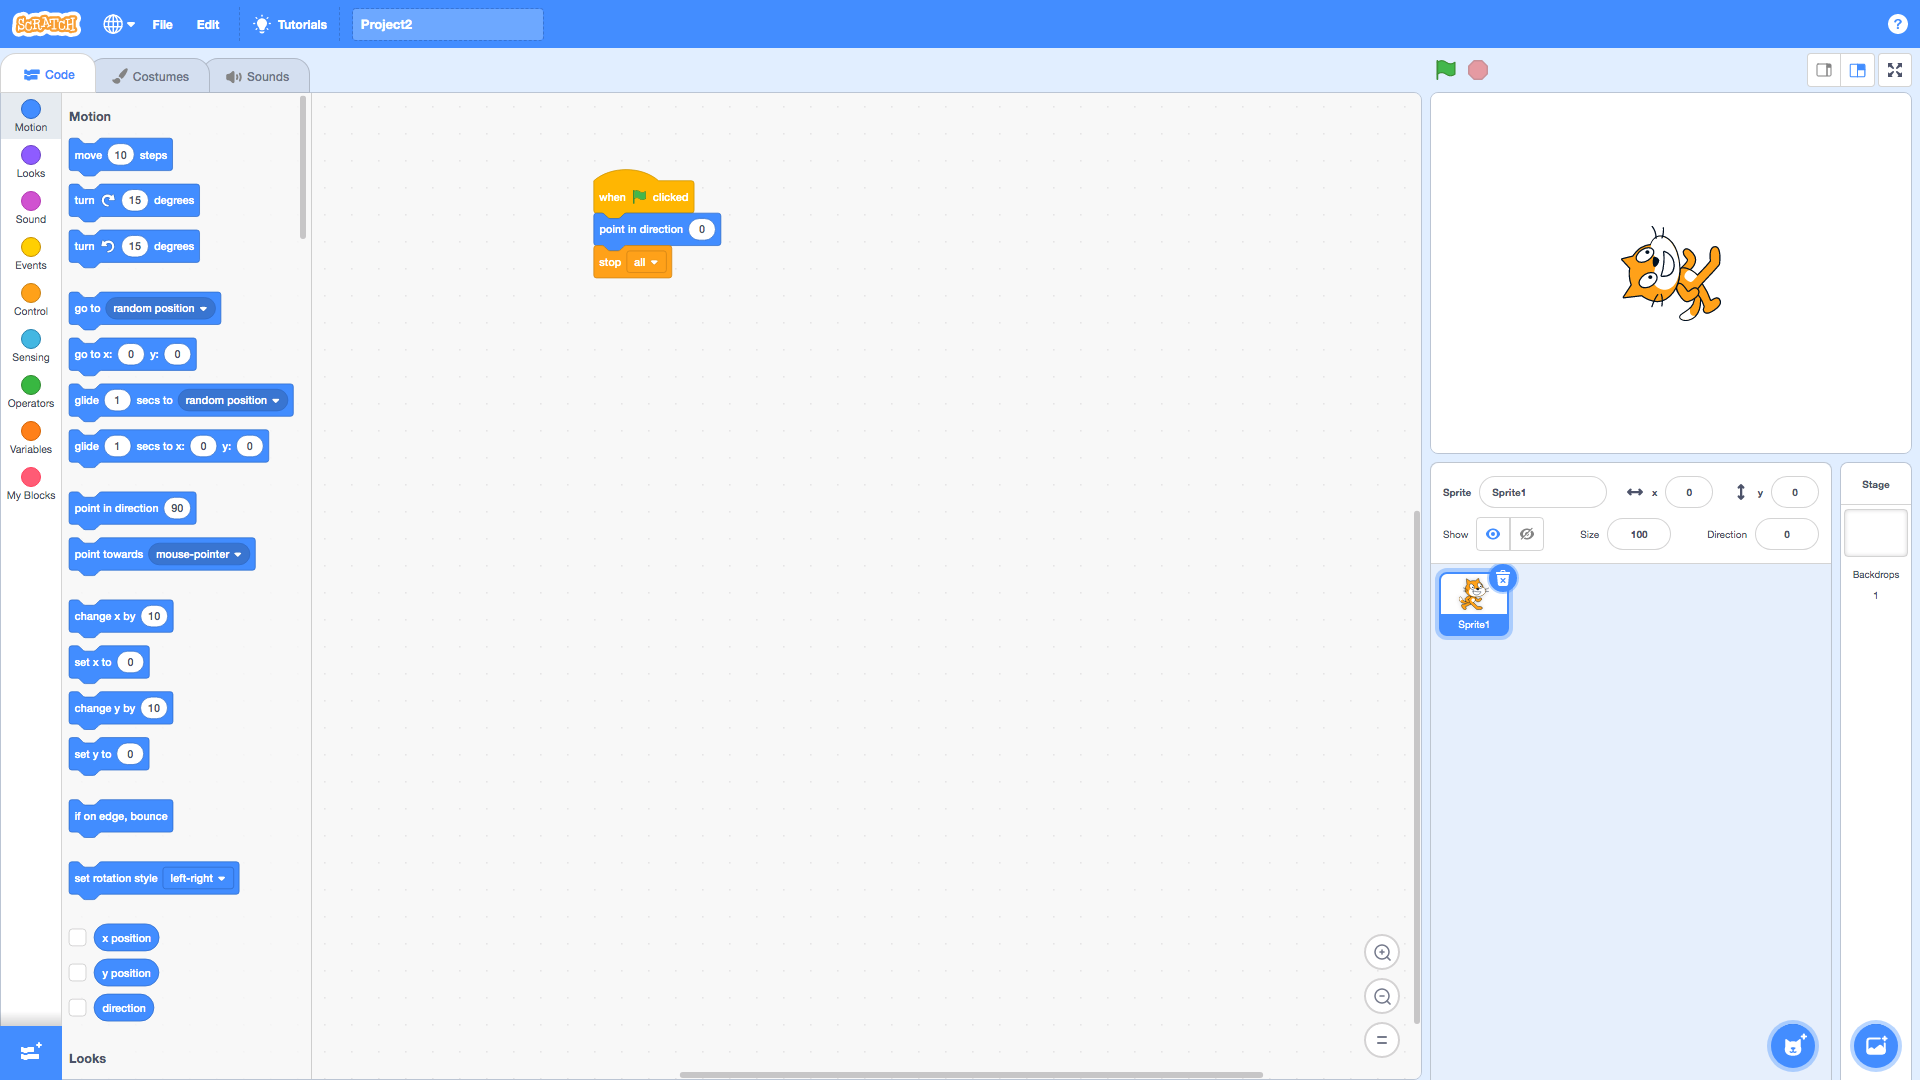
\includegraphics[width=1.0\linewidth,height=0.5\linewidth]{fig020012.png}
  \caption{Ъглова ориентация}
\label{fig020012}
\end{figure}

При по-сложни сценарии за управление на героя, понякога е нужно героят да следи показалеца на мишката. За тази цел има определено блокче, което изпълнява тази инструкция (Фиг. \ref{fig020013}).

\begin{figure}[H]
  \centering
  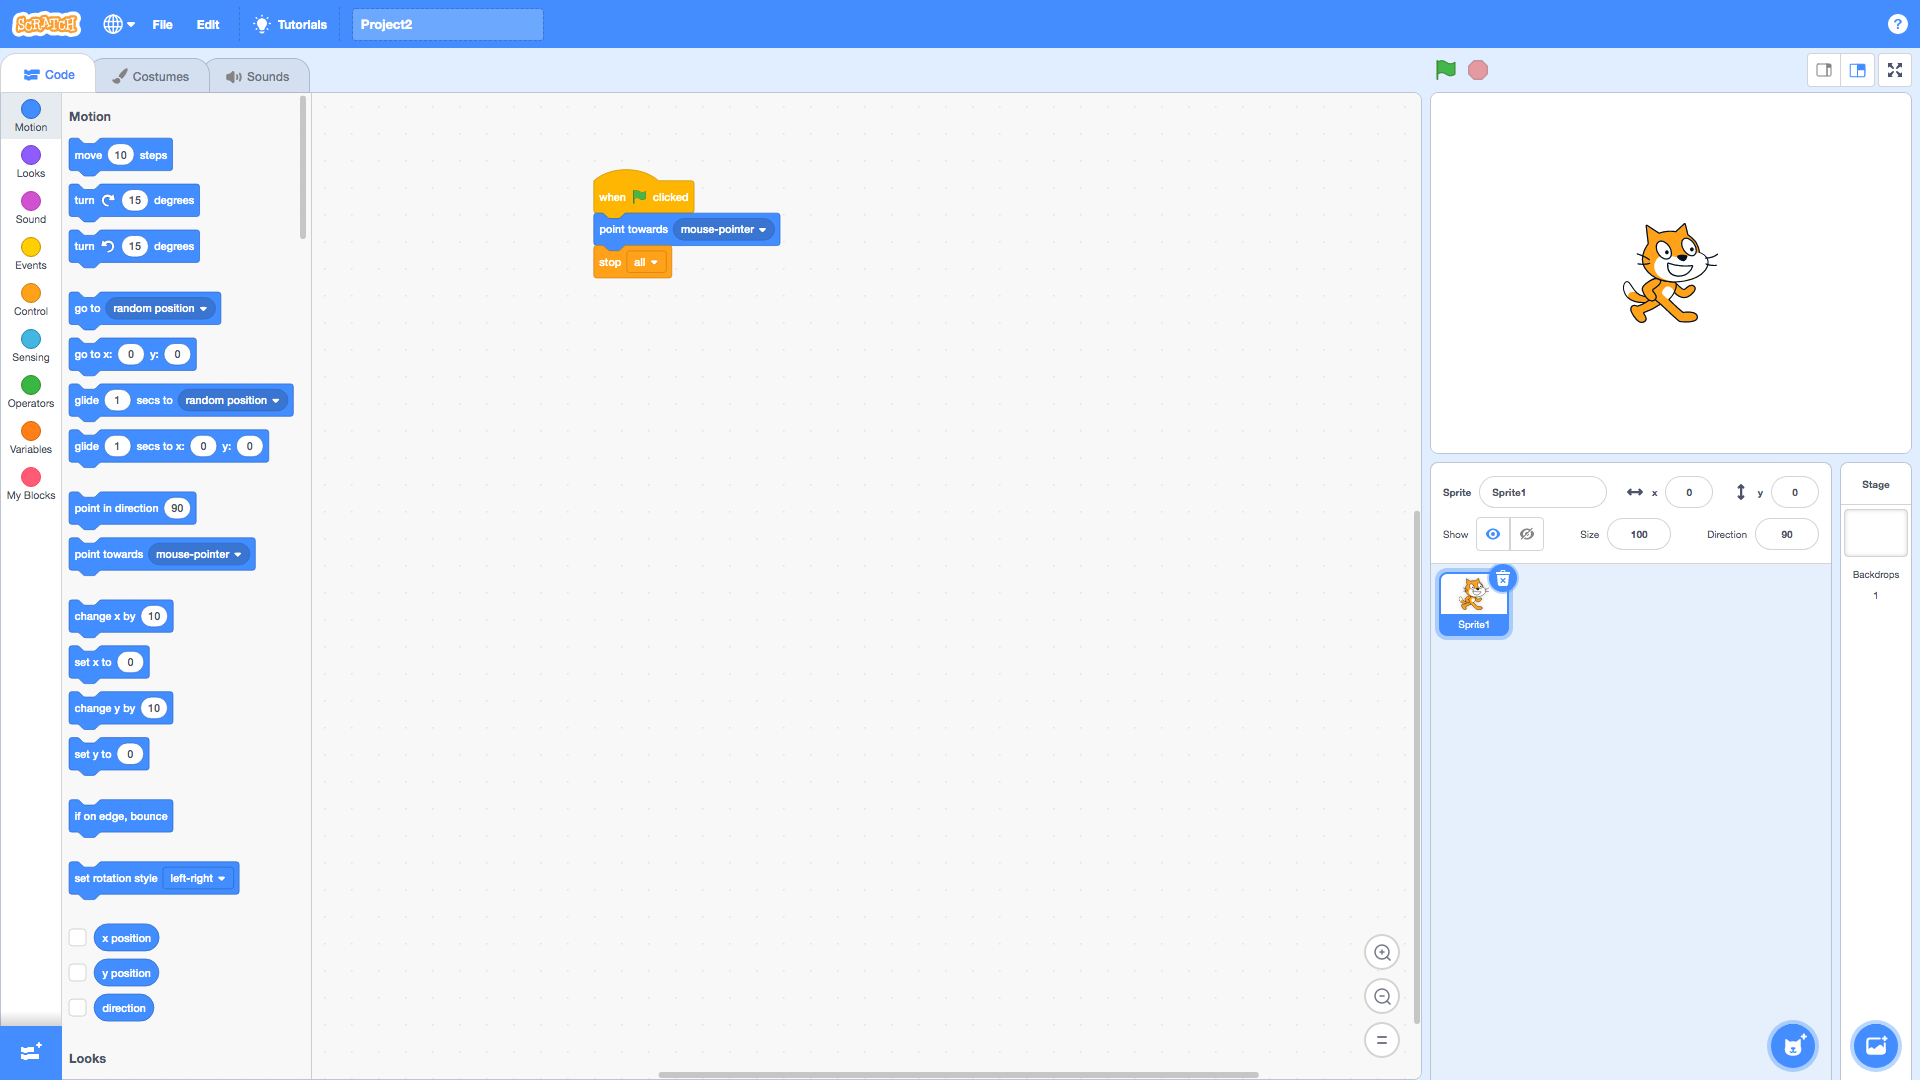
\includegraphics[width=1.0\linewidth,height=0.5\linewidth]{fig020013.png}
  \caption{Ориентация по показалеца на мишката}
\label{fig020013}
\end{figure}

Блокчетата могат да се поставят едно след друго, като за последователна промяна на относителните x и y координатите (относителни, спрямо текущата позиция) на героя има специално определени блокчета (Фиг. \ref{fig020014}).

\begin{figure}[H]
  \centering
  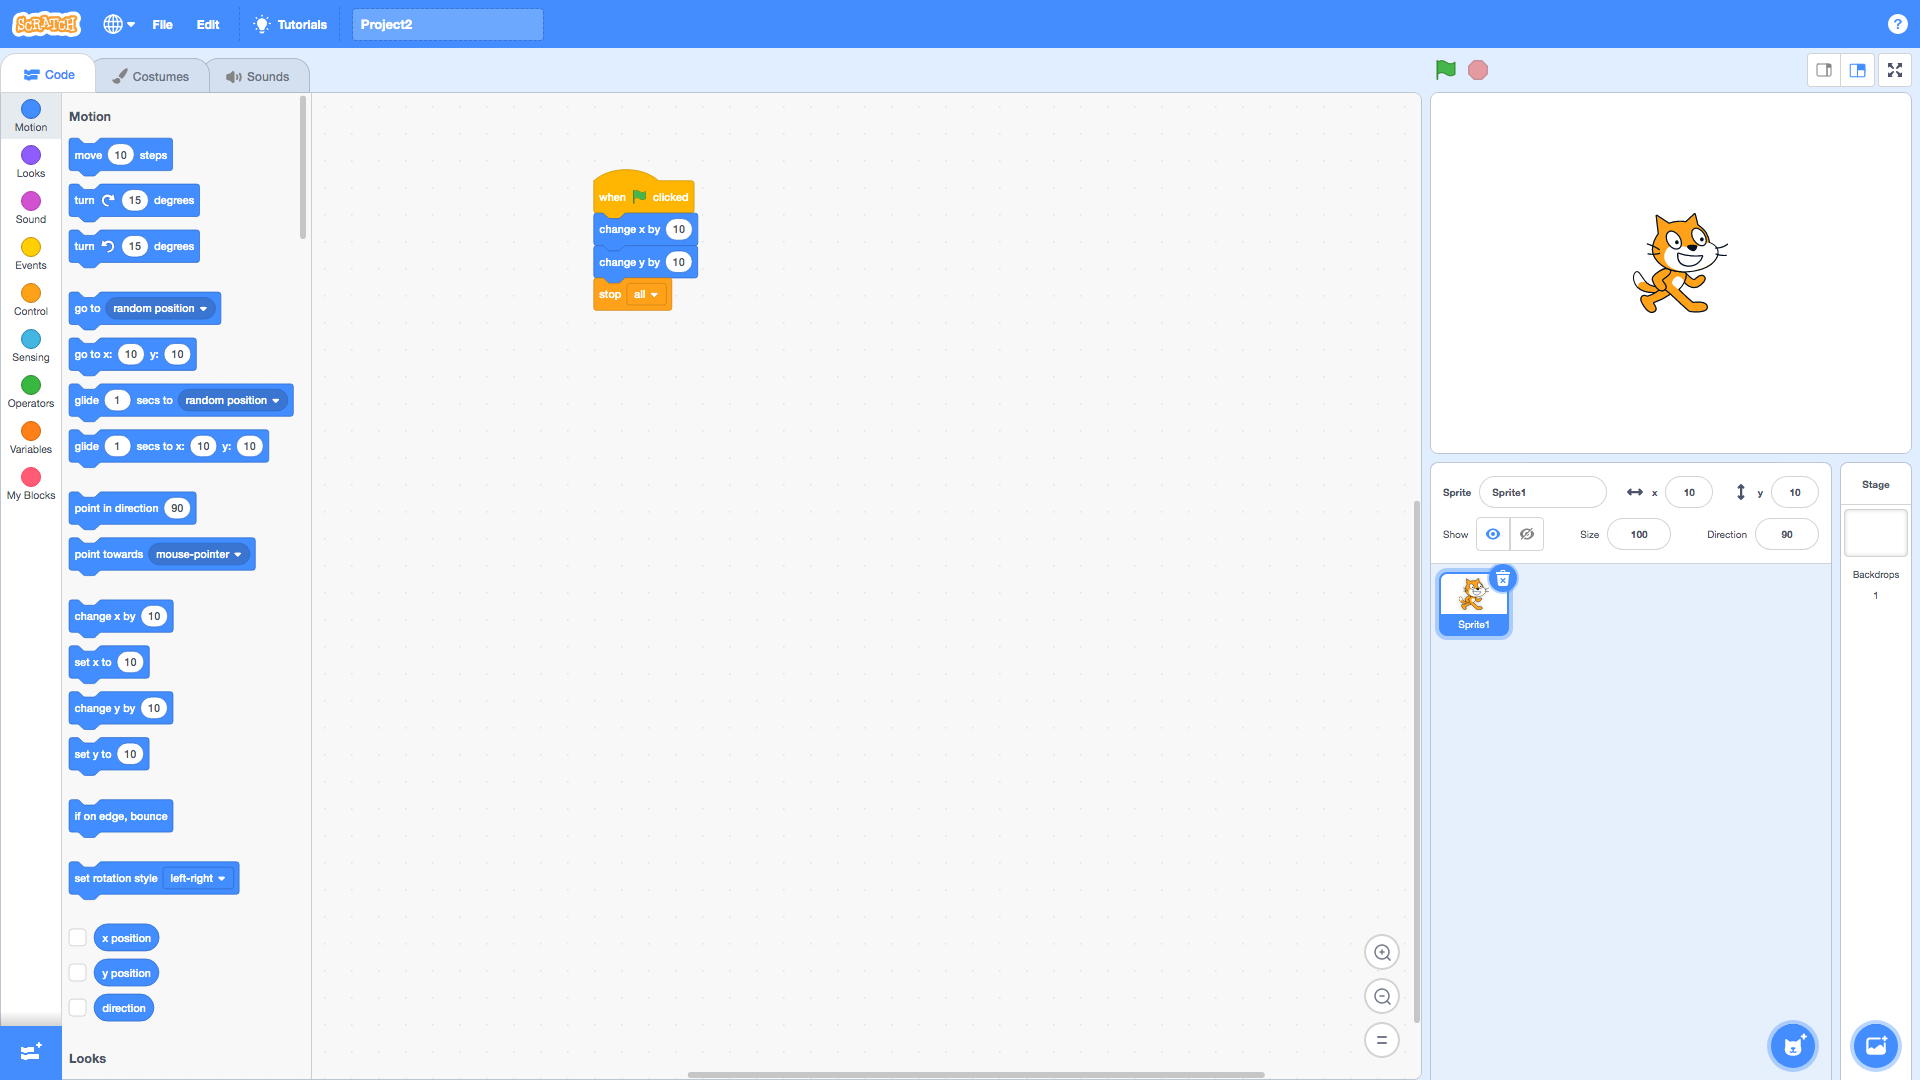
\includegraphics[width=1.0\linewidth,height=0.5\linewidth]{fig020014.png}
  \caption{Последователна промяна на относителни координати}
\label{fig020014}
\end{figure}

Освен относителна промяна на координатите е възможна и абсолютна промяна на координатите, като абсолютната промяна е спрямо центъра на координатната система (Фиг. \ref{fig020015}).

\begin{figure}[H]
  \centering
  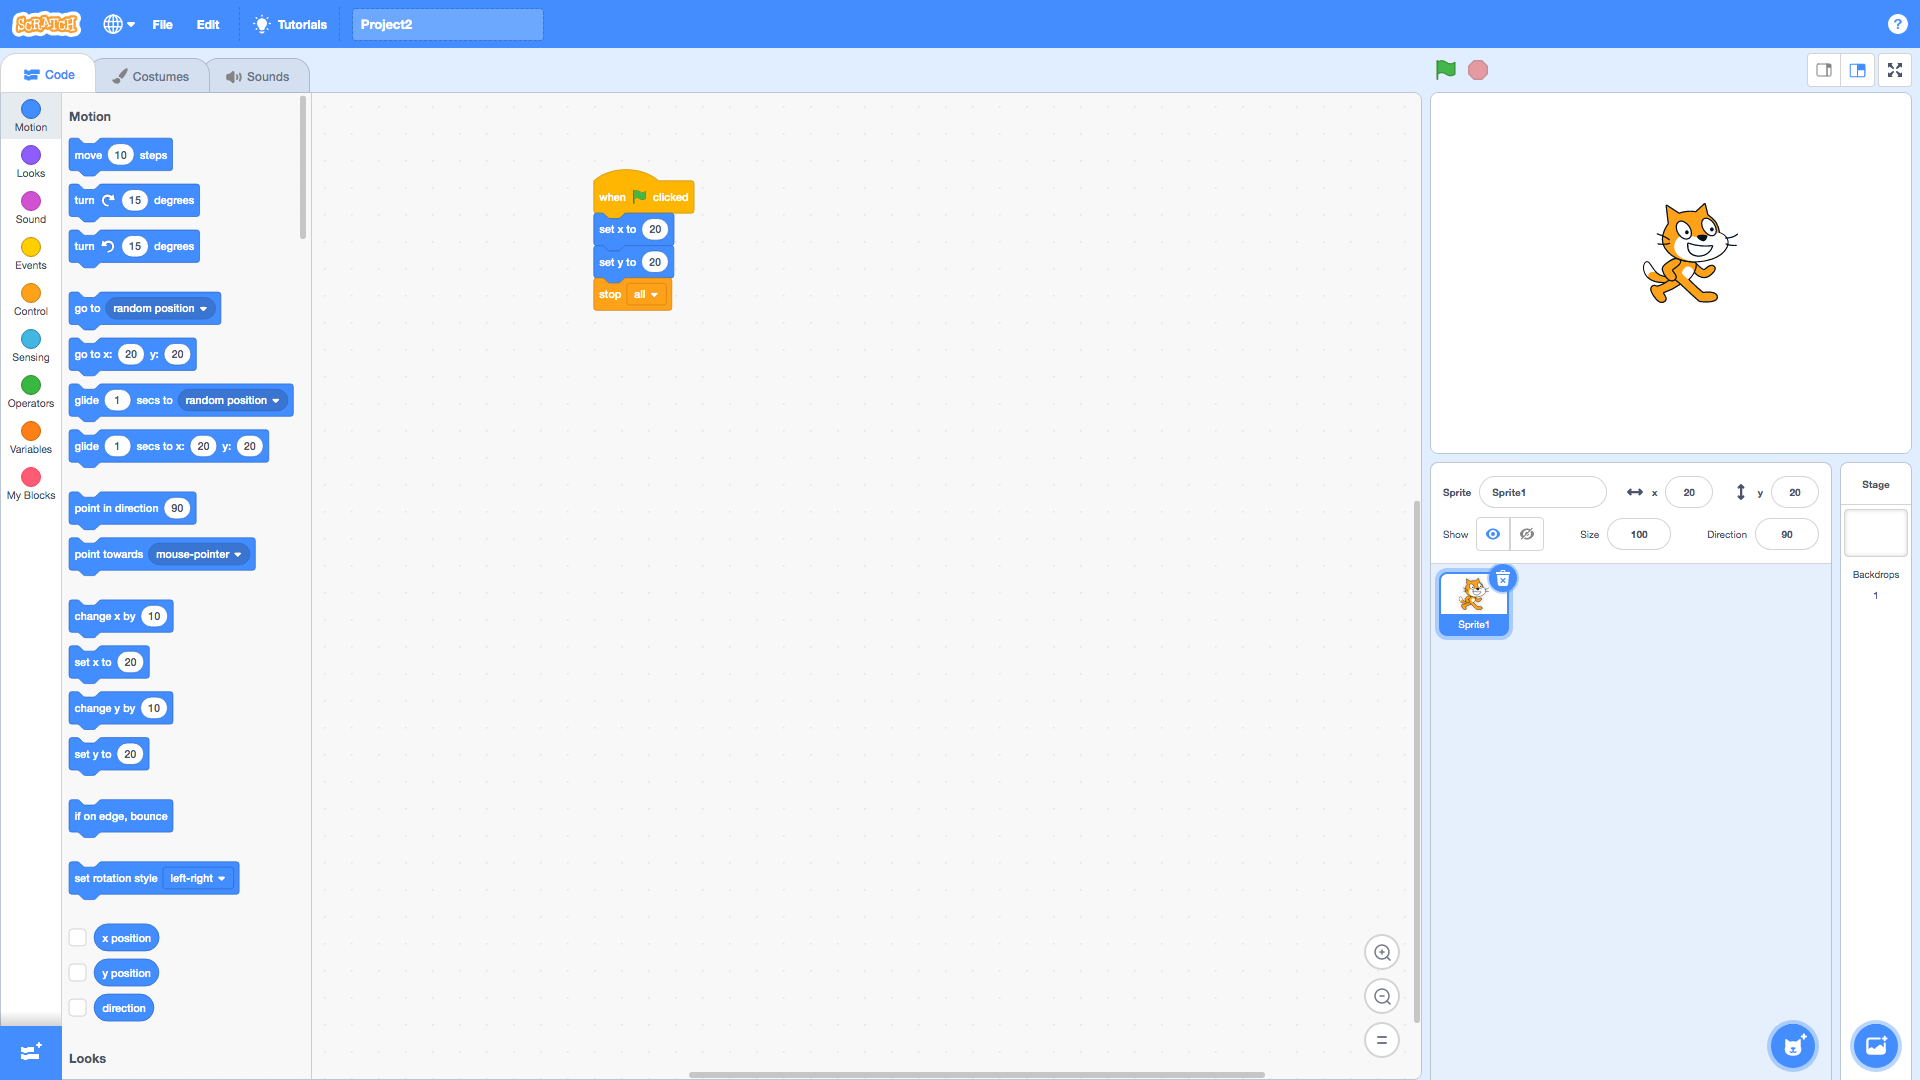
\includegraphics[width=1.0\linewidth,height=0.5\linewidth]{fig020015.png}
  \caption{Последователна промяна на абсолютни координати}
\label{fig020015}
\end{figure}

При своето движение, когато анимираният герой достигне границите на работното пространство, единият вариант е движението да продължи извън видимата зона. Другият вариант е да се вземат мерки и героят да отскача от ръбовете на работното пространство. За това отскачане има конкретно блокче (Фиг. \ref{fig020016}). За да се илюстрира работата му е нужна малко по-сложна последователност от инструкции. При всяко стартиране на програмата, първо се променят относителните координати, а след това се извършва отскачане от ръба, ако е необходимо. За да бъде малко по-интересен сценарият за проверка, вместо фиксирани стойности за относително отместване се използва вграждане на едно от зелените блокчета, което позволява генериране на случайно число в предварително определен диапазон. Съществено е да се забележи, че зеленото блокче има овална форма, което подсказва, че то е предназначено за вграждане в някой от другите блокове, които имат овален слот. 

\begin{figure}[H]
  \centering
  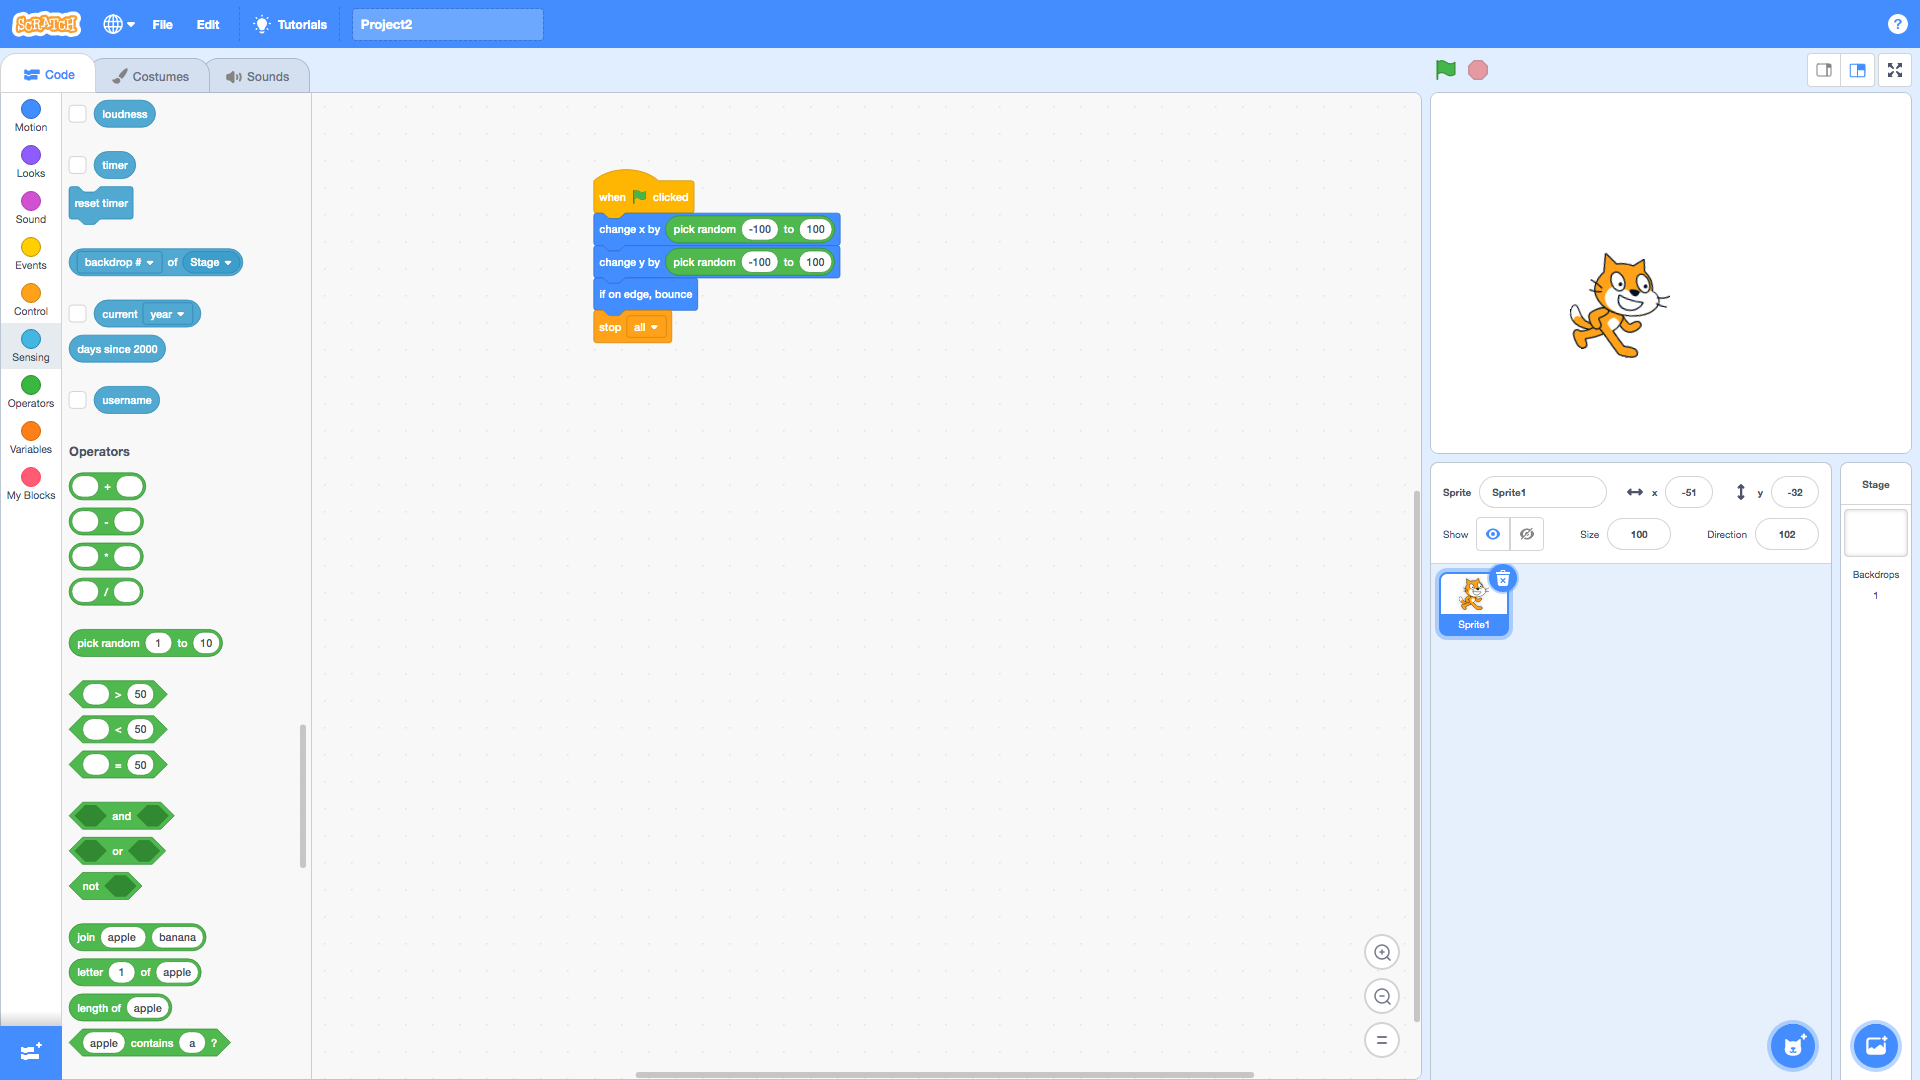
\includegraphics[width=1.0\linewidth,height=0.5\linewidth]{fig020016.png}
  \caption{Отскачане от ръбовете}
\label{fig020016}
\end{figure}

Следващо, много полезно блокче, от групата на тъмно оранжевите е блокчето за изчакване на период от време (Фиг. \ref{fig020017}). Когато това блокче бъде поставено между блокчетата за начало и край, програмата изчаква зададения брой секунди, преди да преустанови изпълнението си. По време на изпълнение, ясно може да се забележи, че около последователността от инструкции се появява жълта рамка, която символизира режима на изпълняващи се инструкции. 

\begin{figure}[H]
  \centering
  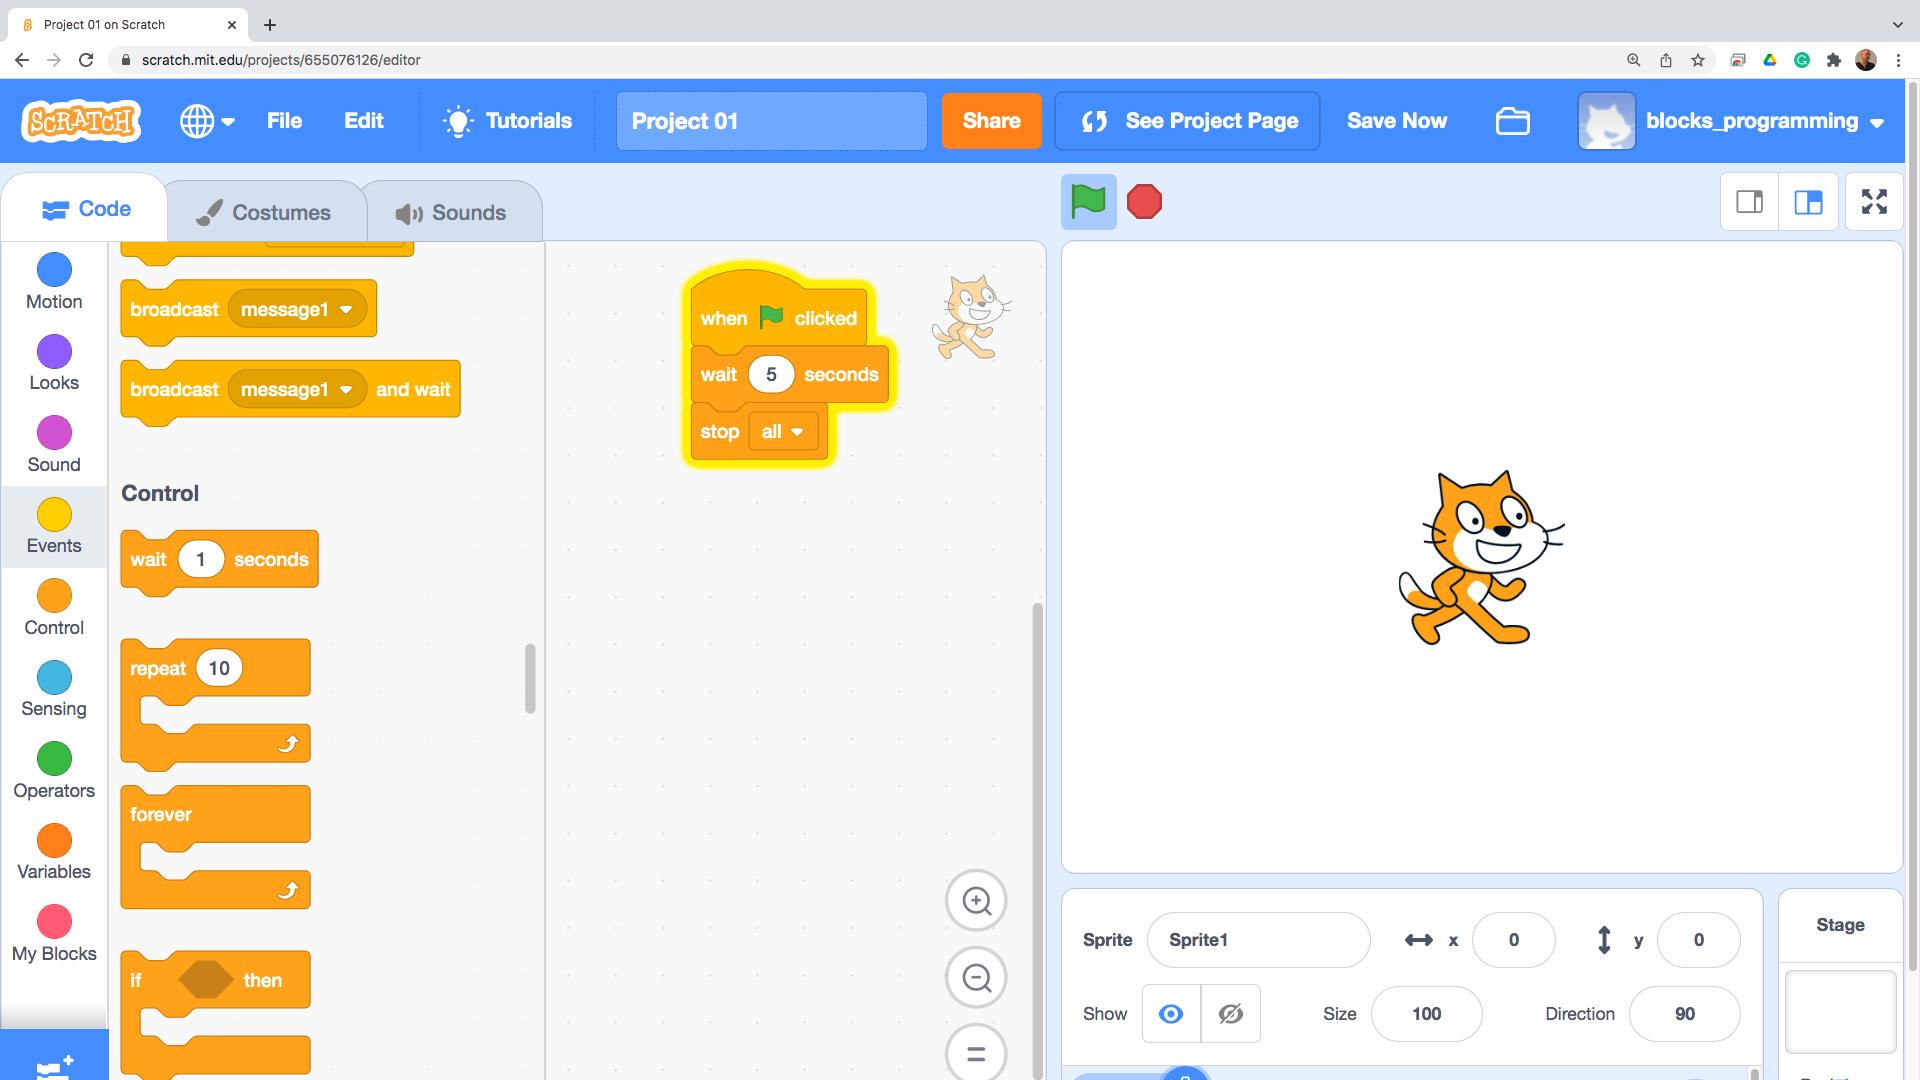
\includegraphics[width=1.0\linewidth,height=0.5\linewidth]{fig020017.png}
  \caption{Инструкция за изчакване}
\label{fig020017}
\end{figure}

Групата на лилавите блокчета съдържат инструкции за външното оформление на анимирания герой. Първите две блокчета са предназначени за реплики (Фиг. \ref{fig020018}), които героят казва (изписват се както в комикс). Първото блокче задава текст, който стои на екрана до следващата инструкция. Точно за това е нужно да има няколко секунди изчакване, така че текстът да остане видим за потребителя. Второто блокче има и параметър с който да се определи колко секунди текстът да бъде видим за потребителя. 

\begin{figure}[H]
  \centering
  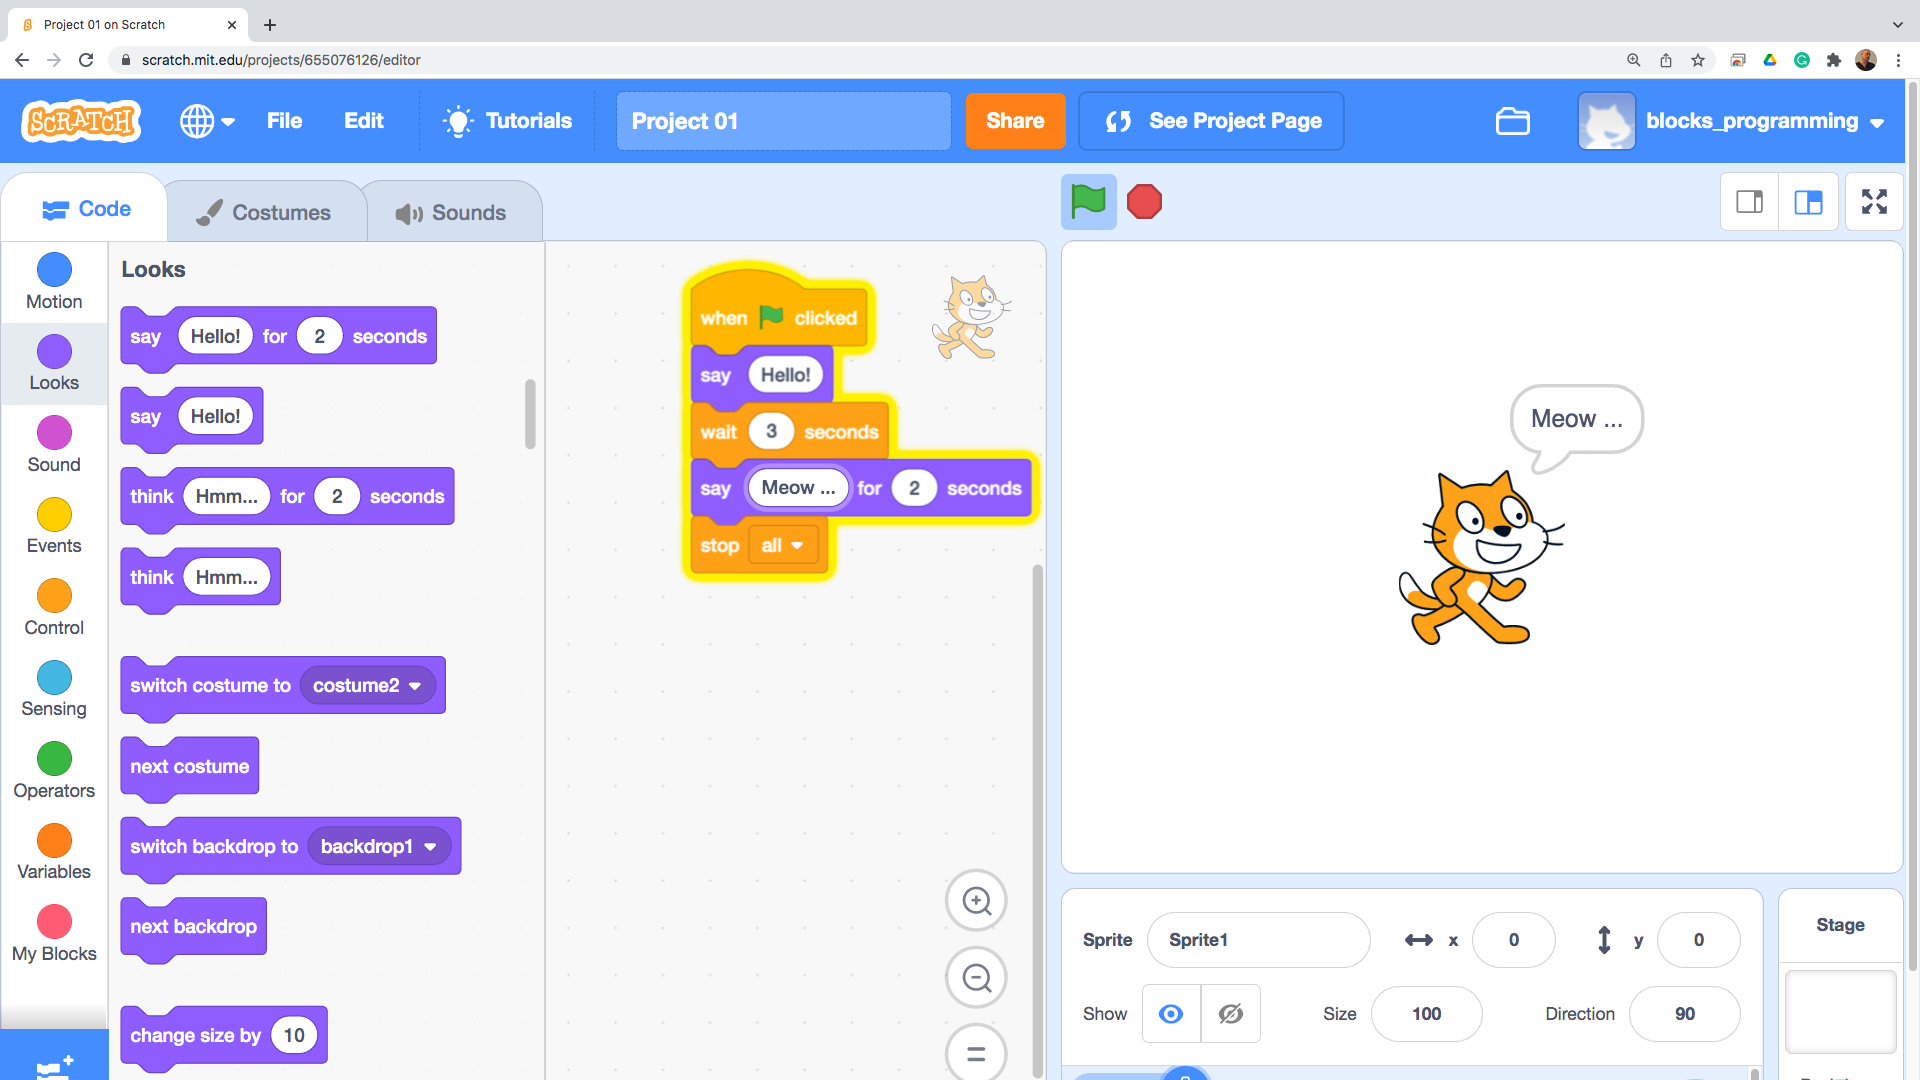
\includegraphics[width=1.0\linewidth,height=0.5\linewidth]{fig020018.png}
  \caption{Изписване на реплики за изговаряне}
\label{fig020018}
\end{figure}

Вторите две блокчета са предвидени за реплики, които анимираният герой си мисли, но не изрича. Разликата се състои в начина по който се визуализира текстът (Фиг. \ref{fig020019}).

\begin{figure}[H]
  \centering
  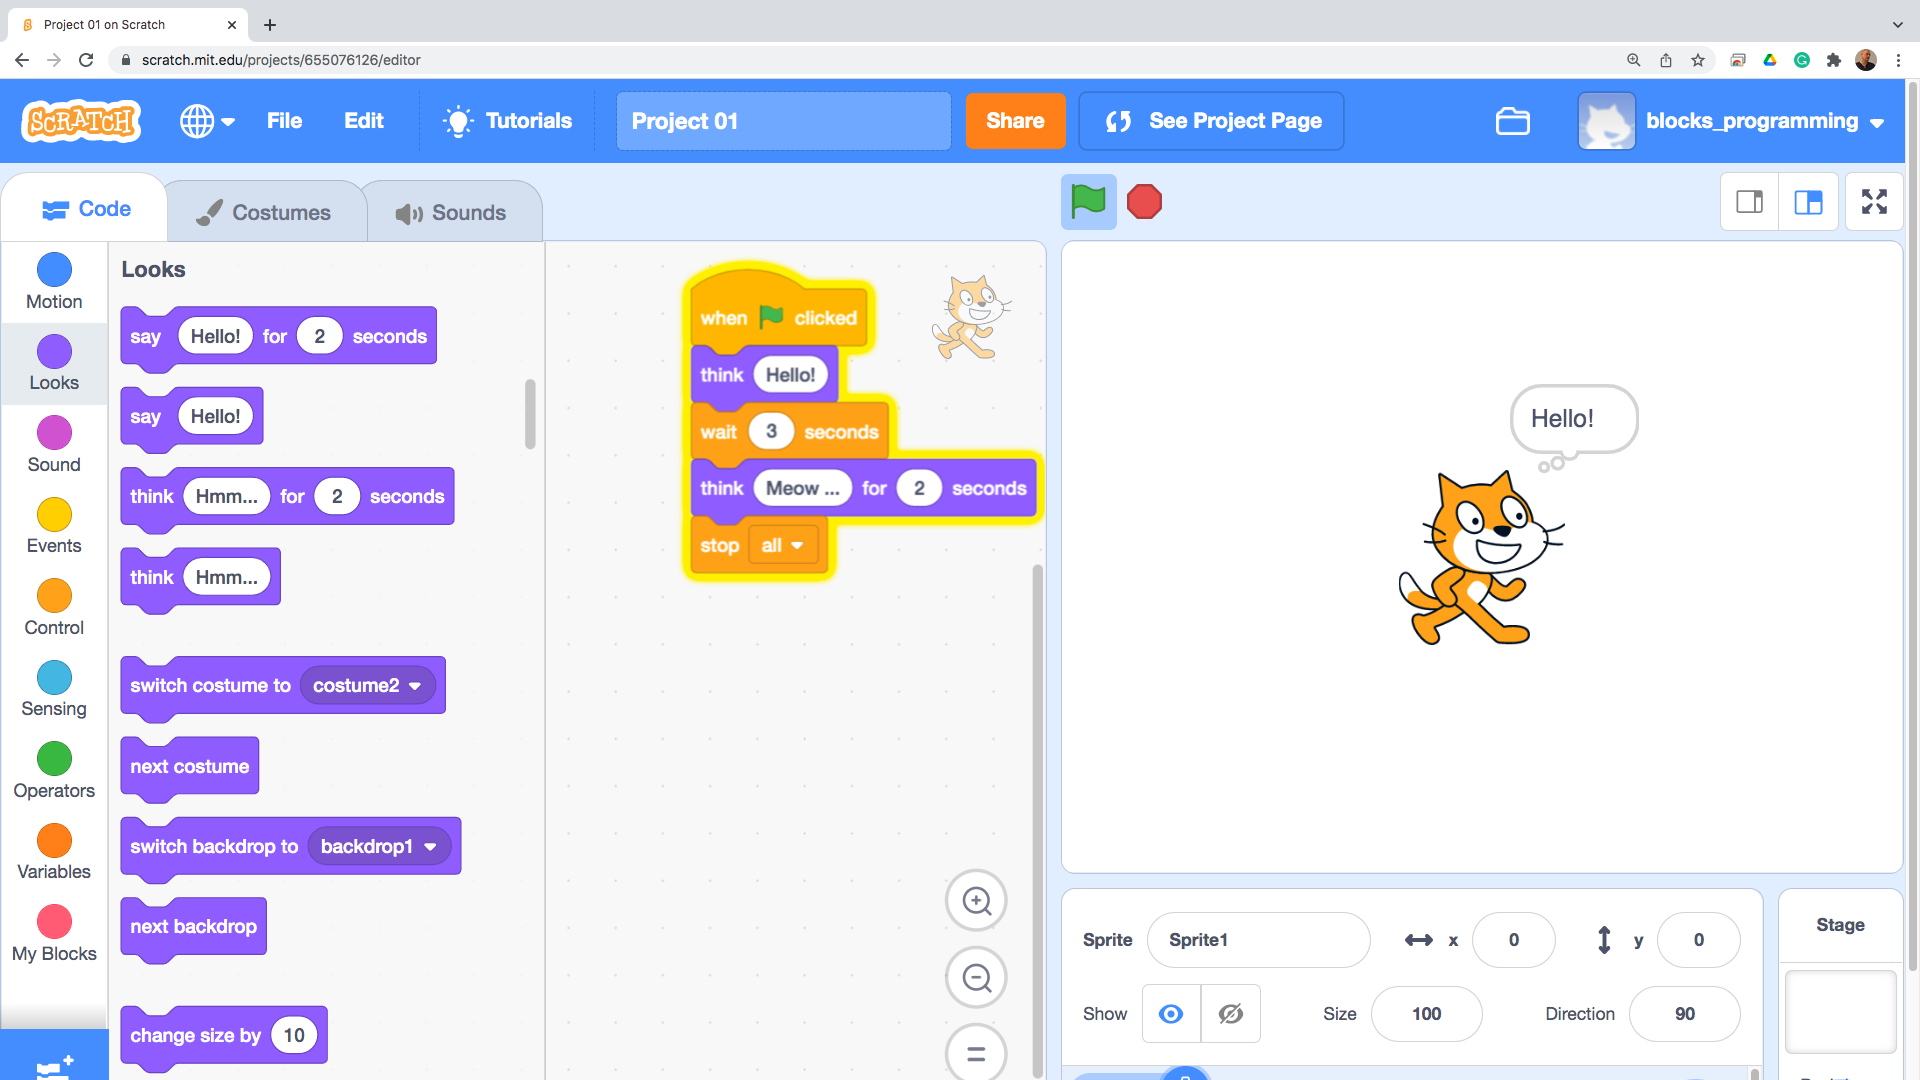
\includegraphics[width=1.0\linewidth,height=0.5\linewidth]{fig020019.png}
  \caption{Изписване на реплики, като мисъл}
\label{fig020019}
\end{figure}

Анимираните герои в Scratch са под формата на спрайтове. Спрайтът е набор от различни изображения за героя в различни пози. За смяната на тези различни пози се използват две блокчета (Фиг. \ref{fig020020}), като първото задава конкретен кадър в спрайта, а второто задава следващия кадър в последователността.

\begin{figure}[H]
  \centering
  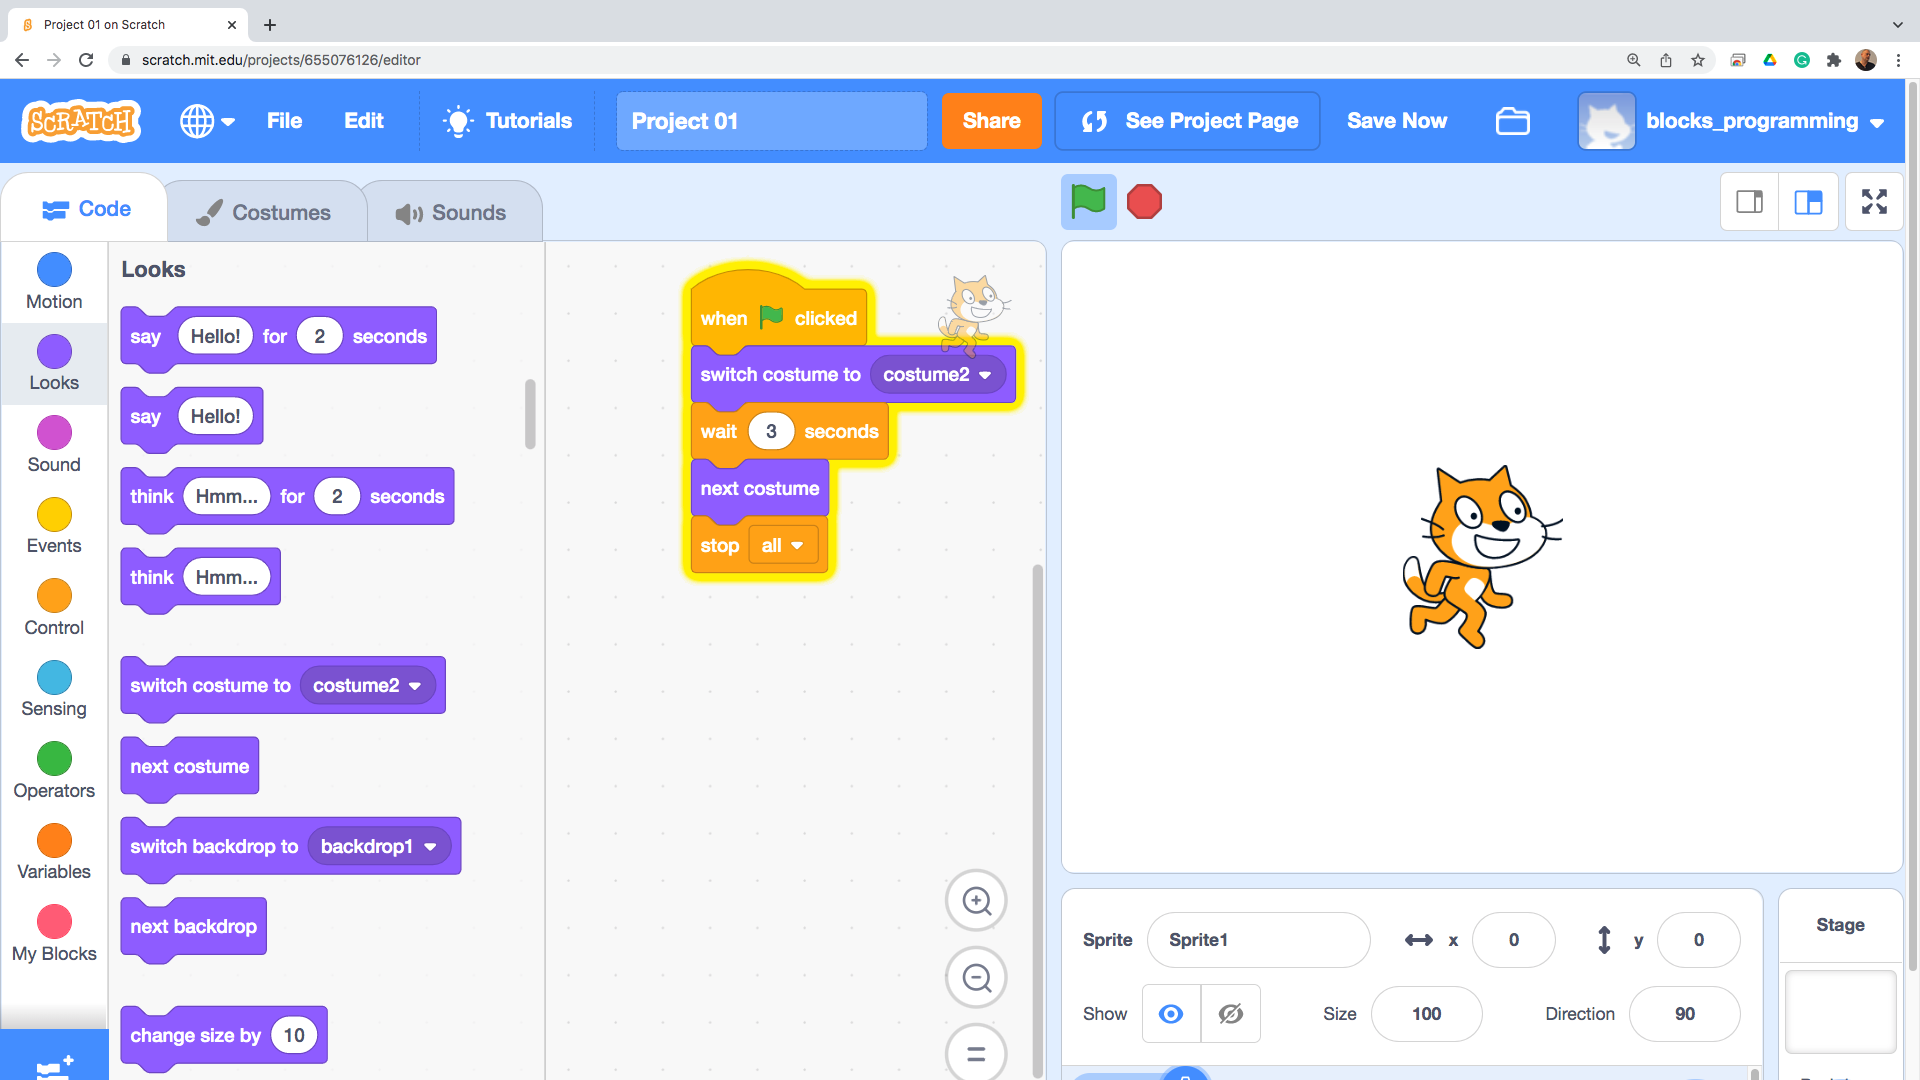
\includegraphics[width=1.0\linewidth,height=0.5\linewidth]{fig020020.png}
  \caption{Смяна на пози}
\label{fig020020}
\end{figure}

На работната сцена освен анимираните герои (под формата на спрайтове) има и фоново изображение. Това фоново изображение също подлежи на промяна, за което са предвидени две отделни блочета (Фиг. \ref{fig020021}). С първото може да се избират фонови изображения напред, назад, по случаен принцип или с конкретно название, а с второто блокче следващото изображение в последователността. 

\begin{figure}[H]
  \centering
  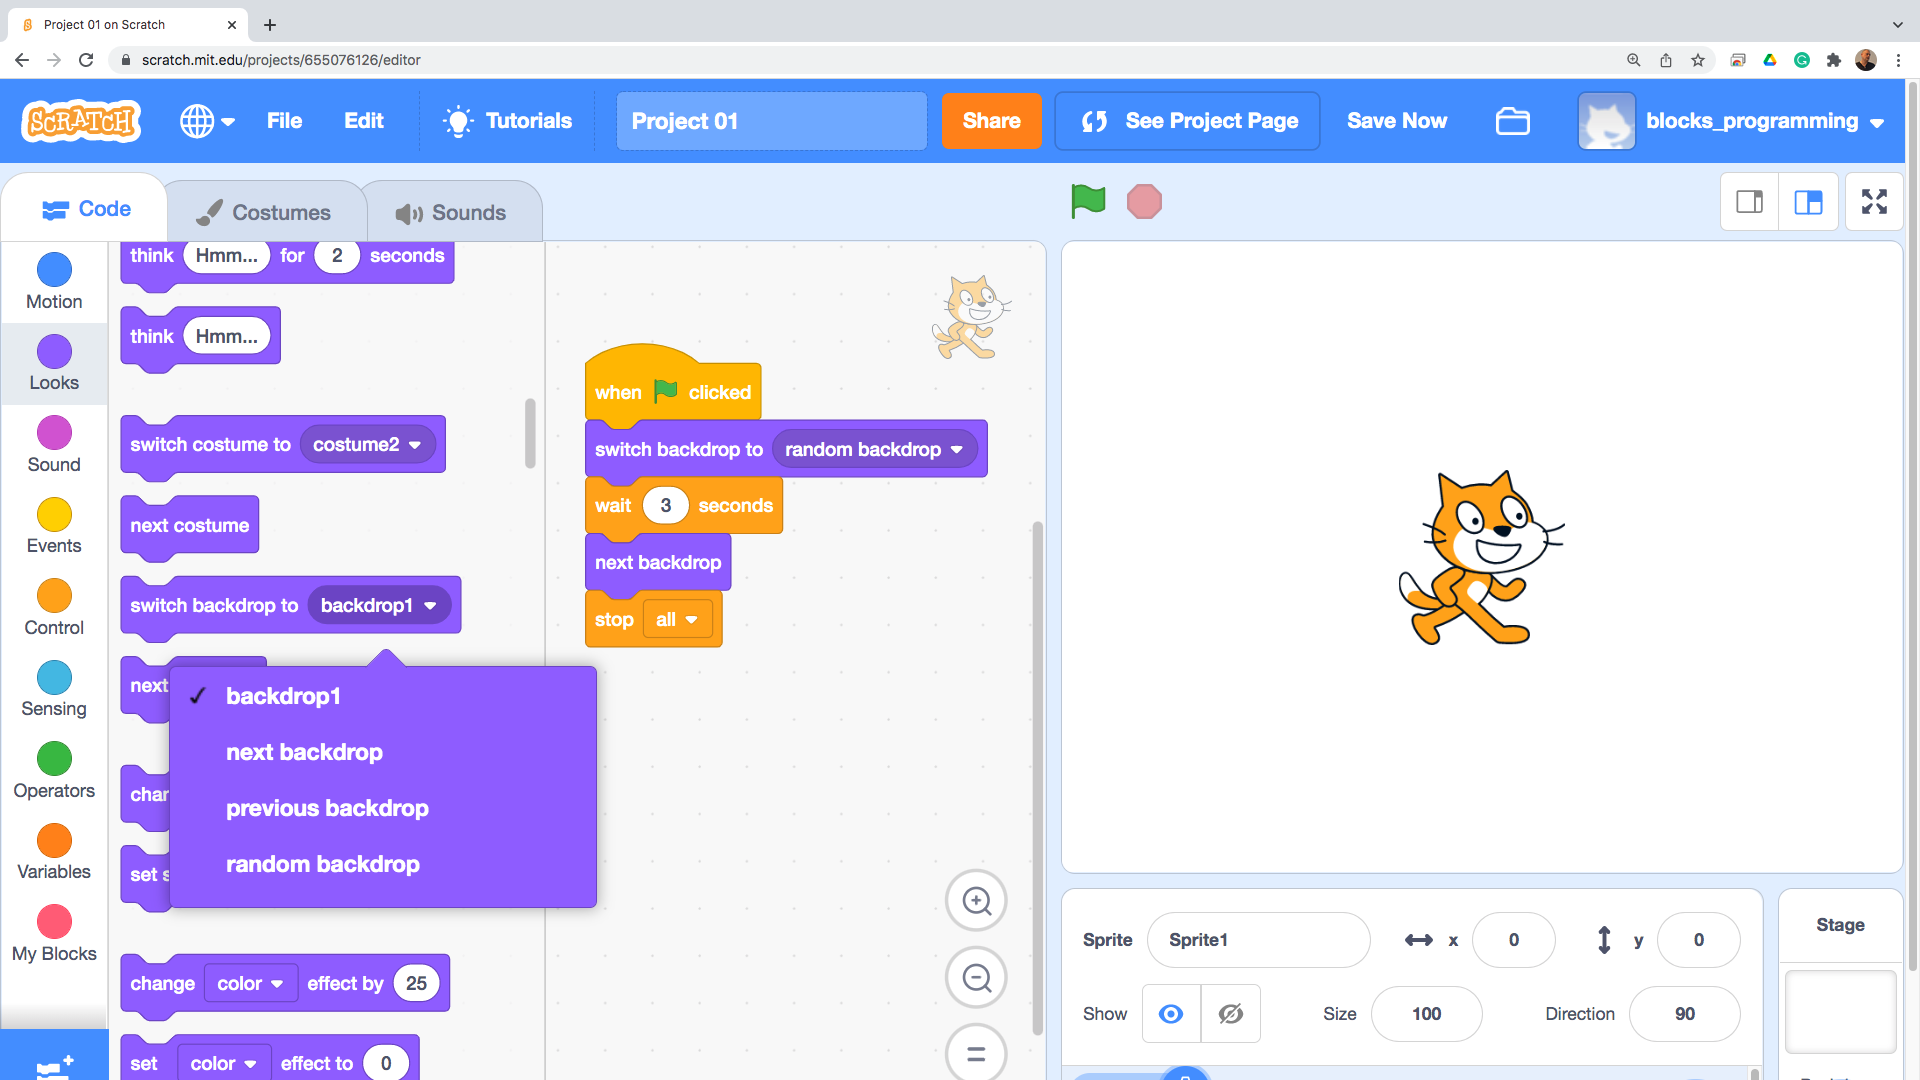
\includegraphics[width=1.0\linewidth,height=0.5\linewidth]{fig020021.png}
  \caption{Смяна на фона}
\label{fig020021}
\end{figure}

За промяната на размера на анимирания герой има две конкретни блокчета, като първото променя размера в абсолютни стойности, а второто променя размера в проценти, спрямо оригиналния размер (Фиг. \ref{fig020022}).

\begin{figure}[H]
  \centering
  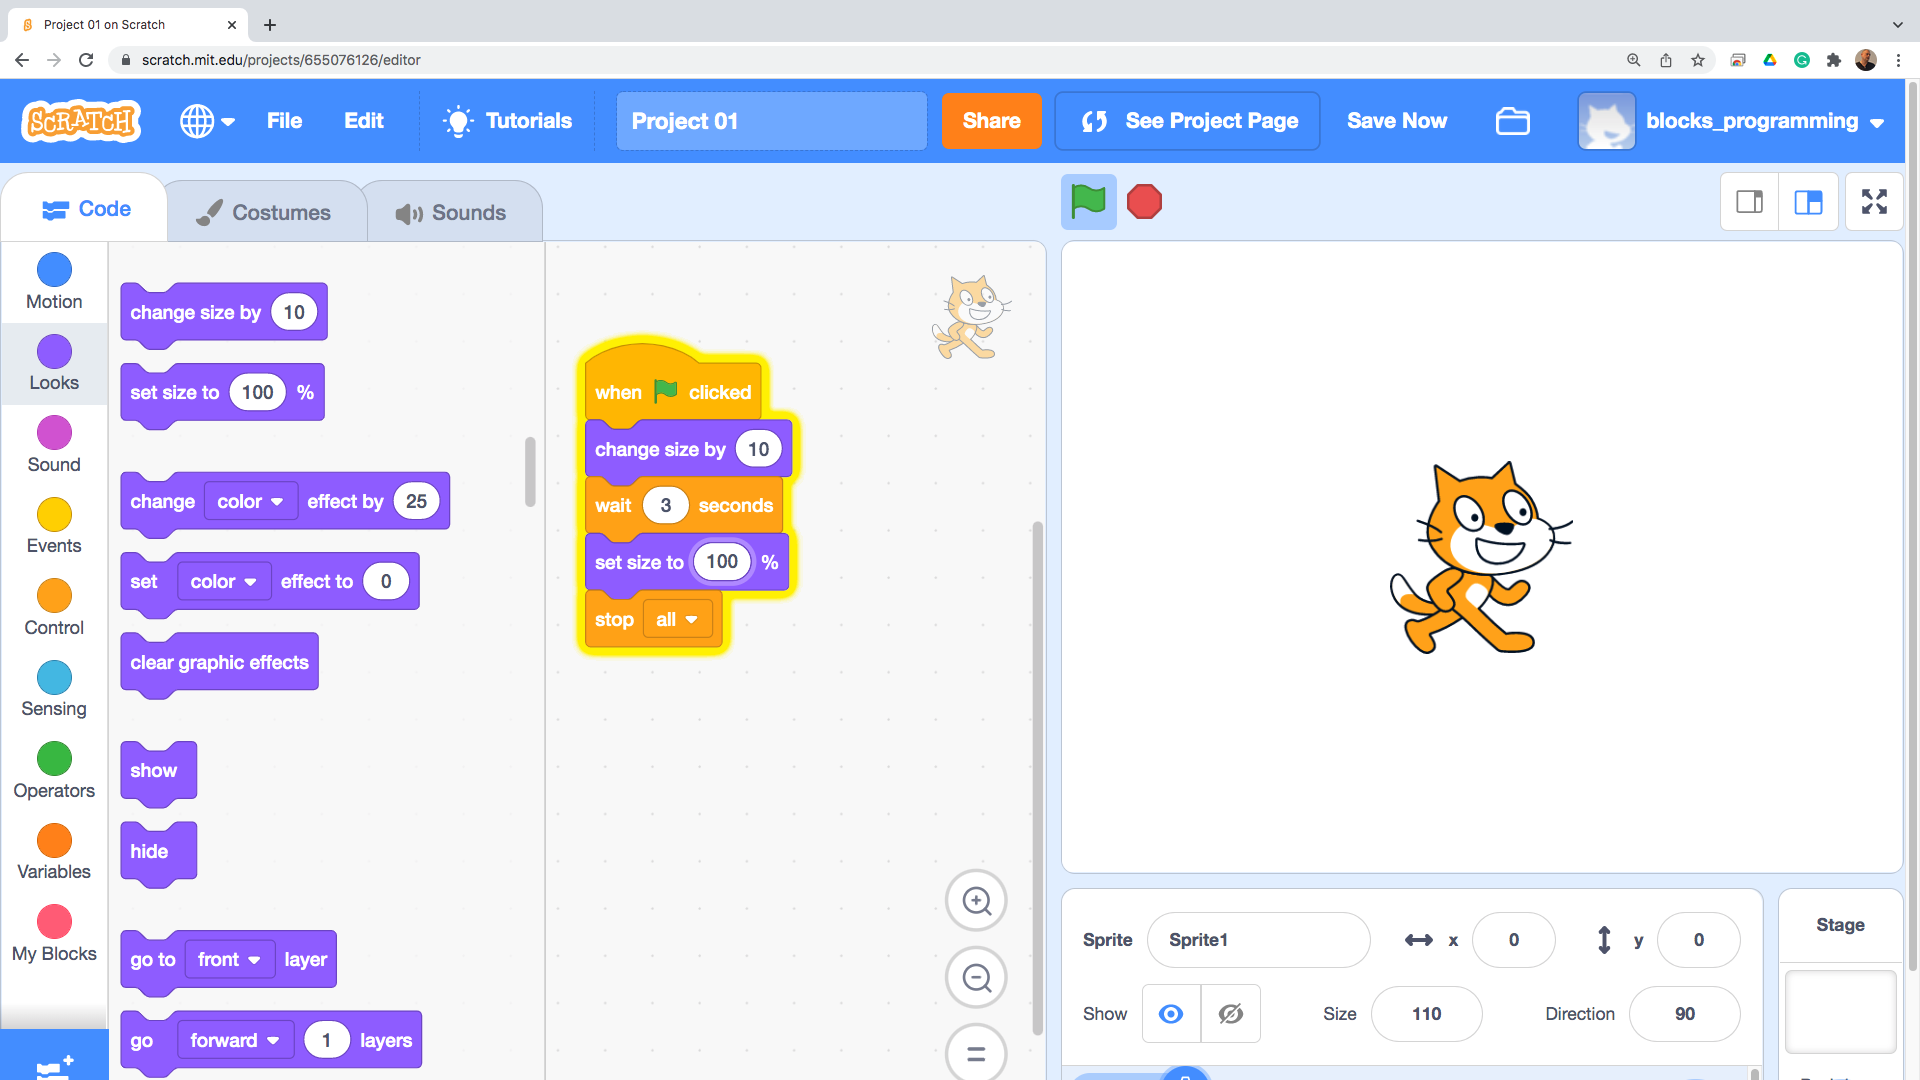
\includegraphics[width=1.0\linewidth,height=0.5\linewidth]{fig020022.png}
  \caption{Промяна на размерите}
\label{fig020022}
\end{figure}

За промяна на визуалното оформление на анимирания герой са предвидени три блокчета (Фиг. \ref{fig020023}). Първите две задават промяна, като промяната може да бъде в цвета, различни изкривявания, пикселизация, мозайка, прозрачност или яркост, а третото блокче отменя всички направени декорации. Първото блокче предизвиква относителна промяна, спрямо текущото състояние на героя, а второто блокче задава абсолютна промяна. Отново е важно да се дадат няколко секунди, така че промените да бъдат ясно различими. 

\begin{figure}[H]
  \centering
  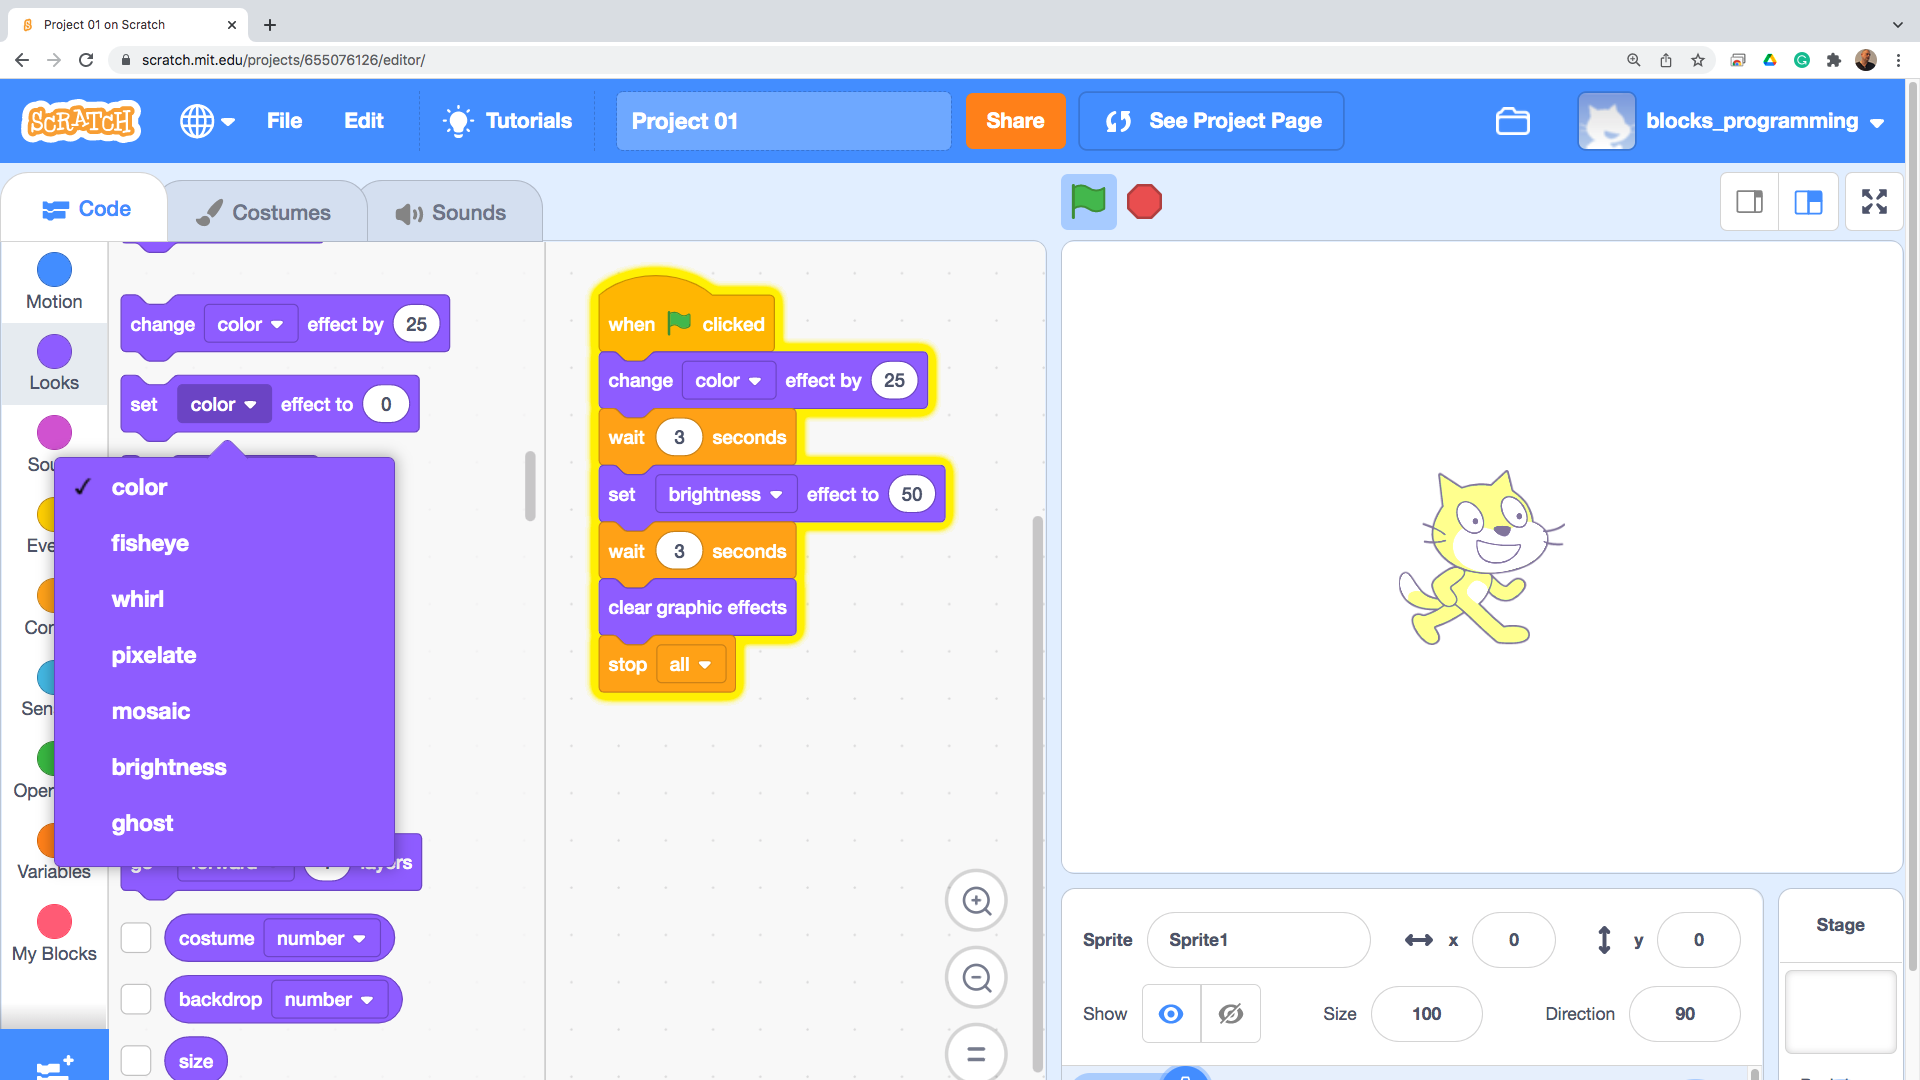
\includegraphics[width=1.0\linewidth,height=0.5\linewidth]{fig020023.png}
  \caption{Промяна на външния вид}
\label{fig020023}
\end{figure}

Работата със спрайтове е предимно за постигане на анимирани ефекти. Различните анимирани герой в сцената имат определени взаимодействия по между си. Сценарият на изработвания проект определя в кой момент всеки от героите се появява на сцената и в кой момент изчезва. За да се осъществи появата и изчезването са предвидени две блокчета, извършващи тези действия (Фиг. \ref{fig020024}).

\begin{figure}[H]
  \centering
  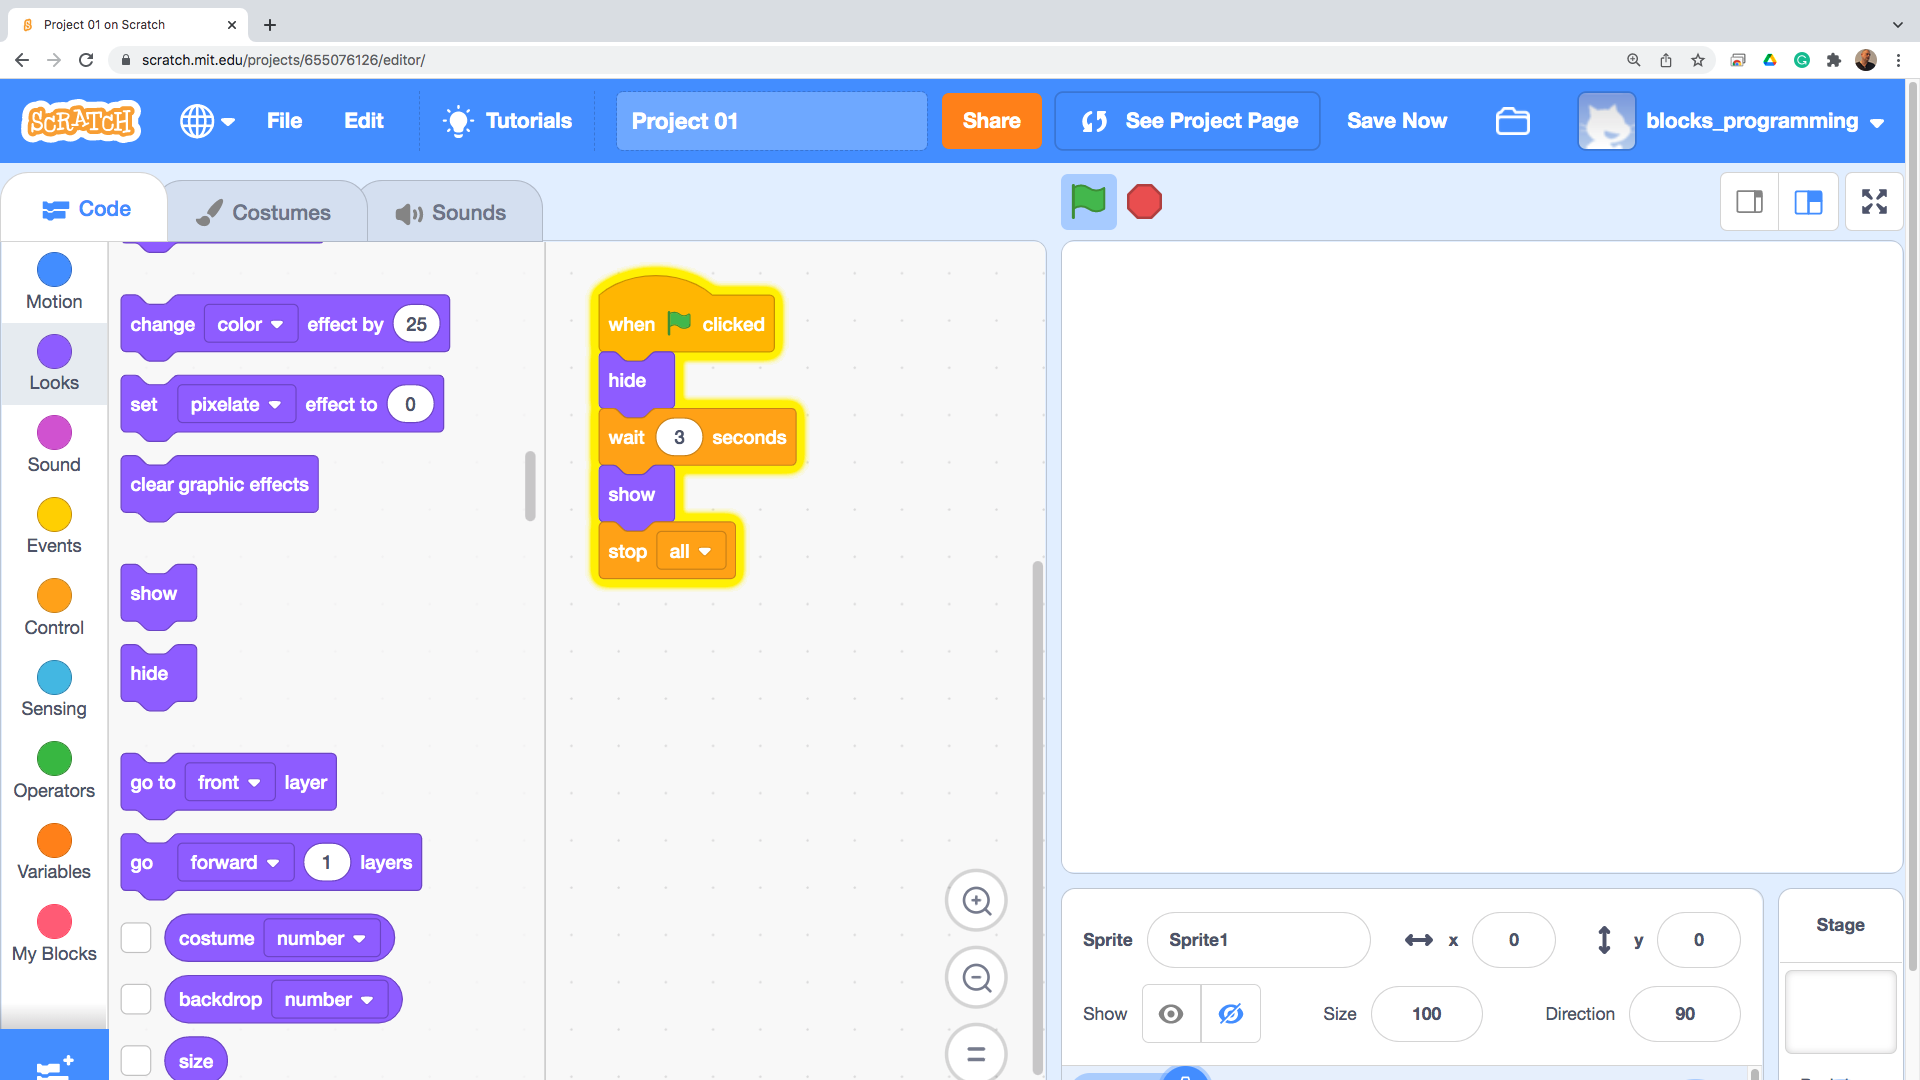
\includegraphics[width=1.0\linewidth,height=0.5\linewidth]{fig020024.png}
  \caption{Скриване и повява}
\label{fig020024}
\end{figure}

Множество програмни продукти, работещи с растерни графични изображения, организират различните изображения в слоеве. Пример за такива са Adobe Photoshop, GIMP, Microsoft Word, LibreOffice Draw и много други. Организацията в слоеве е логична, тъй като различните спрайтове в определени моменти от времето могат да се припокриват. В някои от софтуерните пакети за графична обработка, наличието на слоеве се възприема като Z буфер. В Scratch също е налична възможността за работа със слоеве, като две конкретни блокчета позволяват спрайтът да се придвижва напред и назад по слоевете (Фиг. \ref{fig020025}).

\begin{figure}[H]
  \centering
  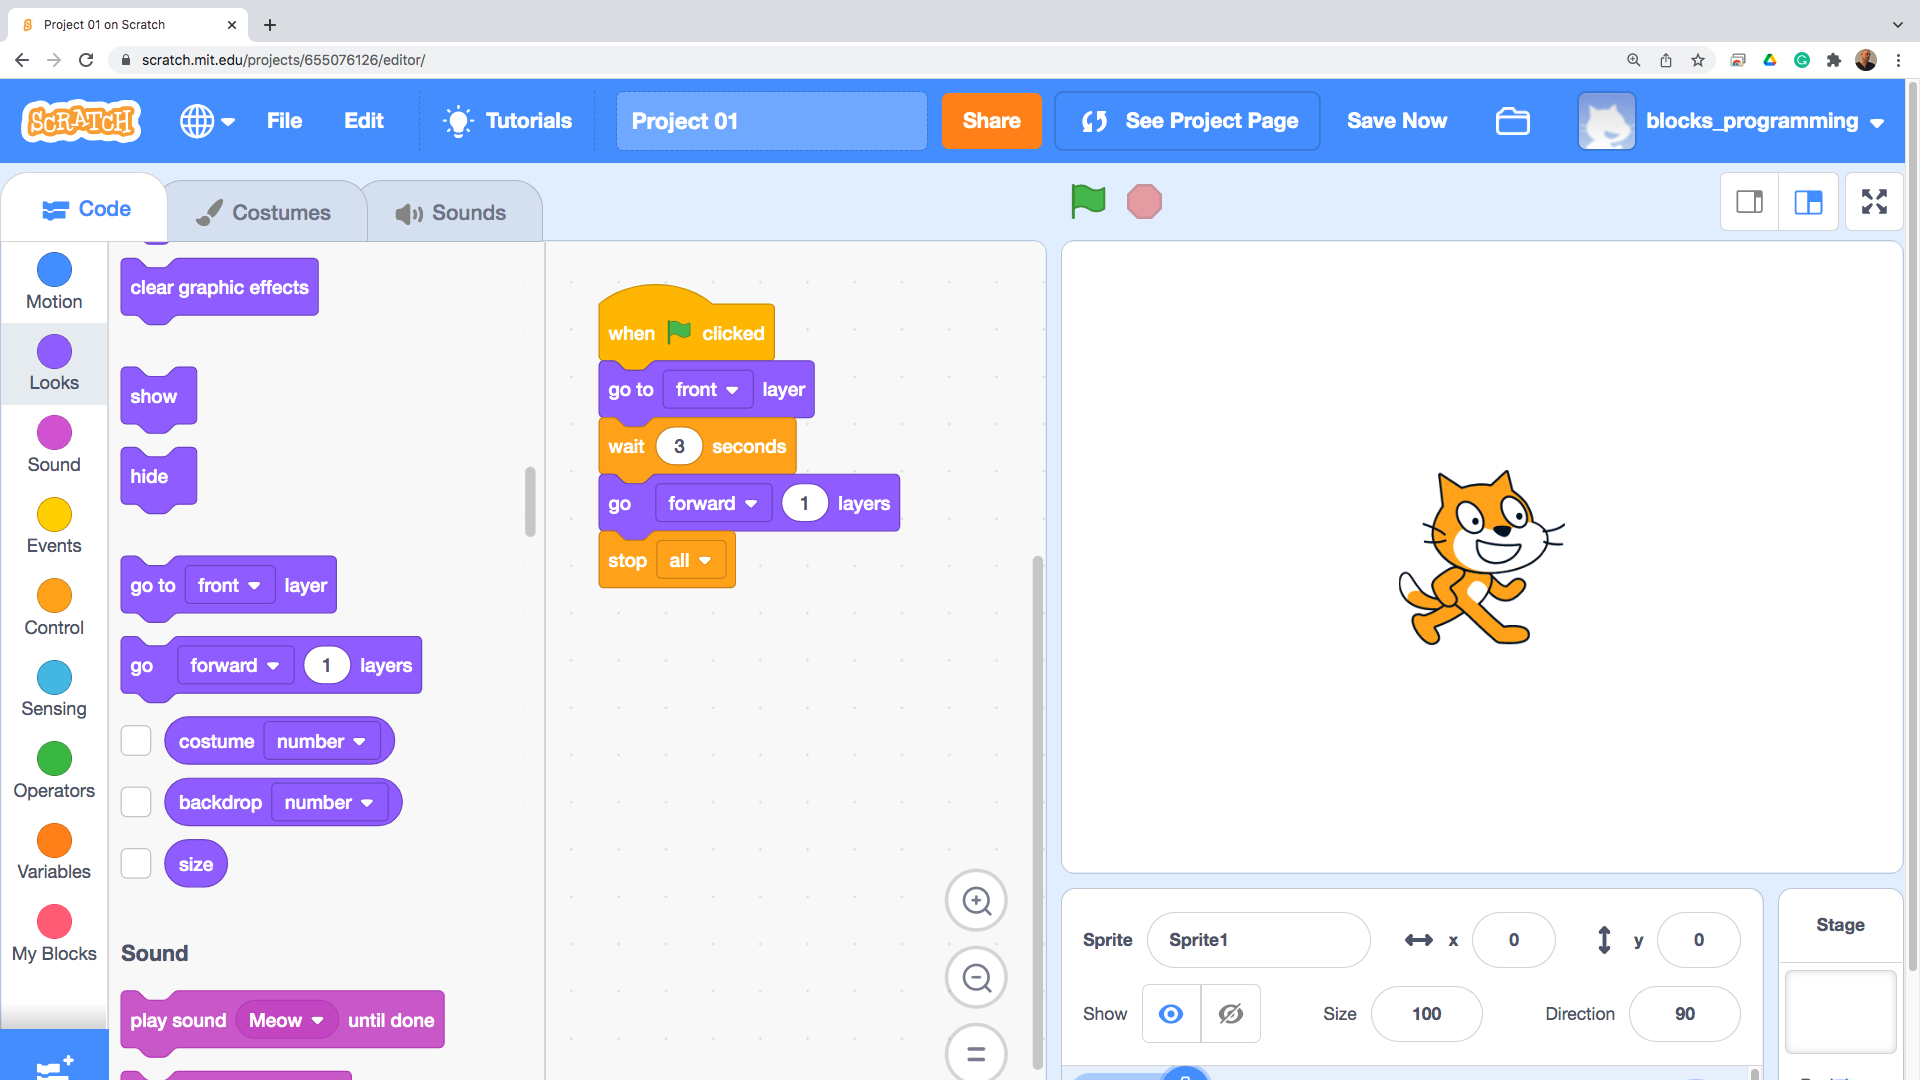
\includegraphics[width=1.0\linewidth,height=0.5\linewidth]{fig020025.png}
  \caption{Придвижване по слоевете}
\label{fig020025}
\end{figure}

Групата блокчета в пурпурен цвят са предназначени за звуково оформление. Изпълнението на звуци се постига с първите две блокчета в групата (Фиг. \ref{fig020026}). Първото блокче изпълнява звука докато той бъде приключен, а второто блокче го стартира и предава изпълнението към следващото блокче. С третото блокче всички изпълняващи се звуци биват спрени. Програмната среда позволява звуци да бъдат записани и от компютъра на потребителя. 

\begin{figure}[H]
  \centering
  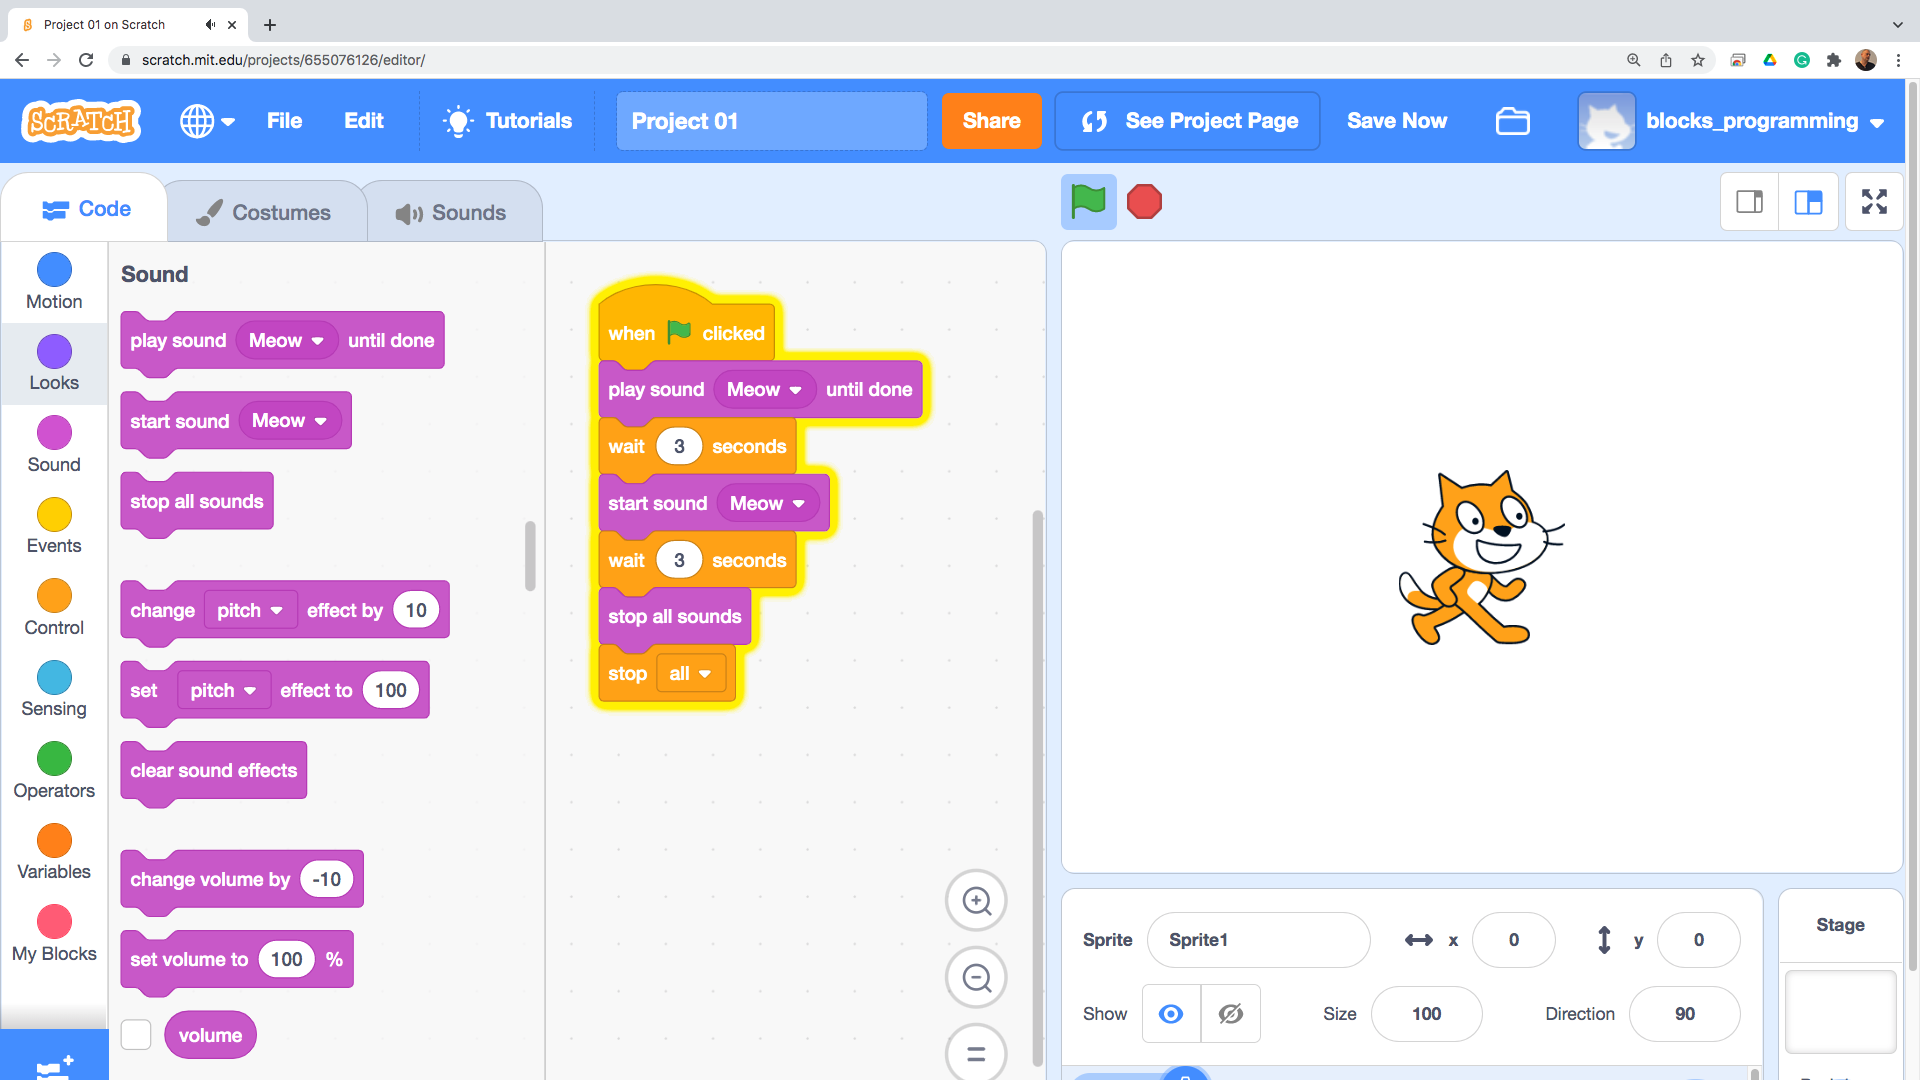
\includegraphics[width=1.0\linewidth,height=0.5\linewidth]{fig020026.png}
  \caption{Изпълнение на звуци}
\label{fig020026}
\end{figure}

Две от характеристиките на звуците могат да се променят с блокчетата за височина (честотна) и стерео озвучаване (ляво/дясно). И двете блокчета имат числени стойности за посочените характеристики (Фиг. \ref{fig020027}).

\begin{figure}[H]
  \centering
  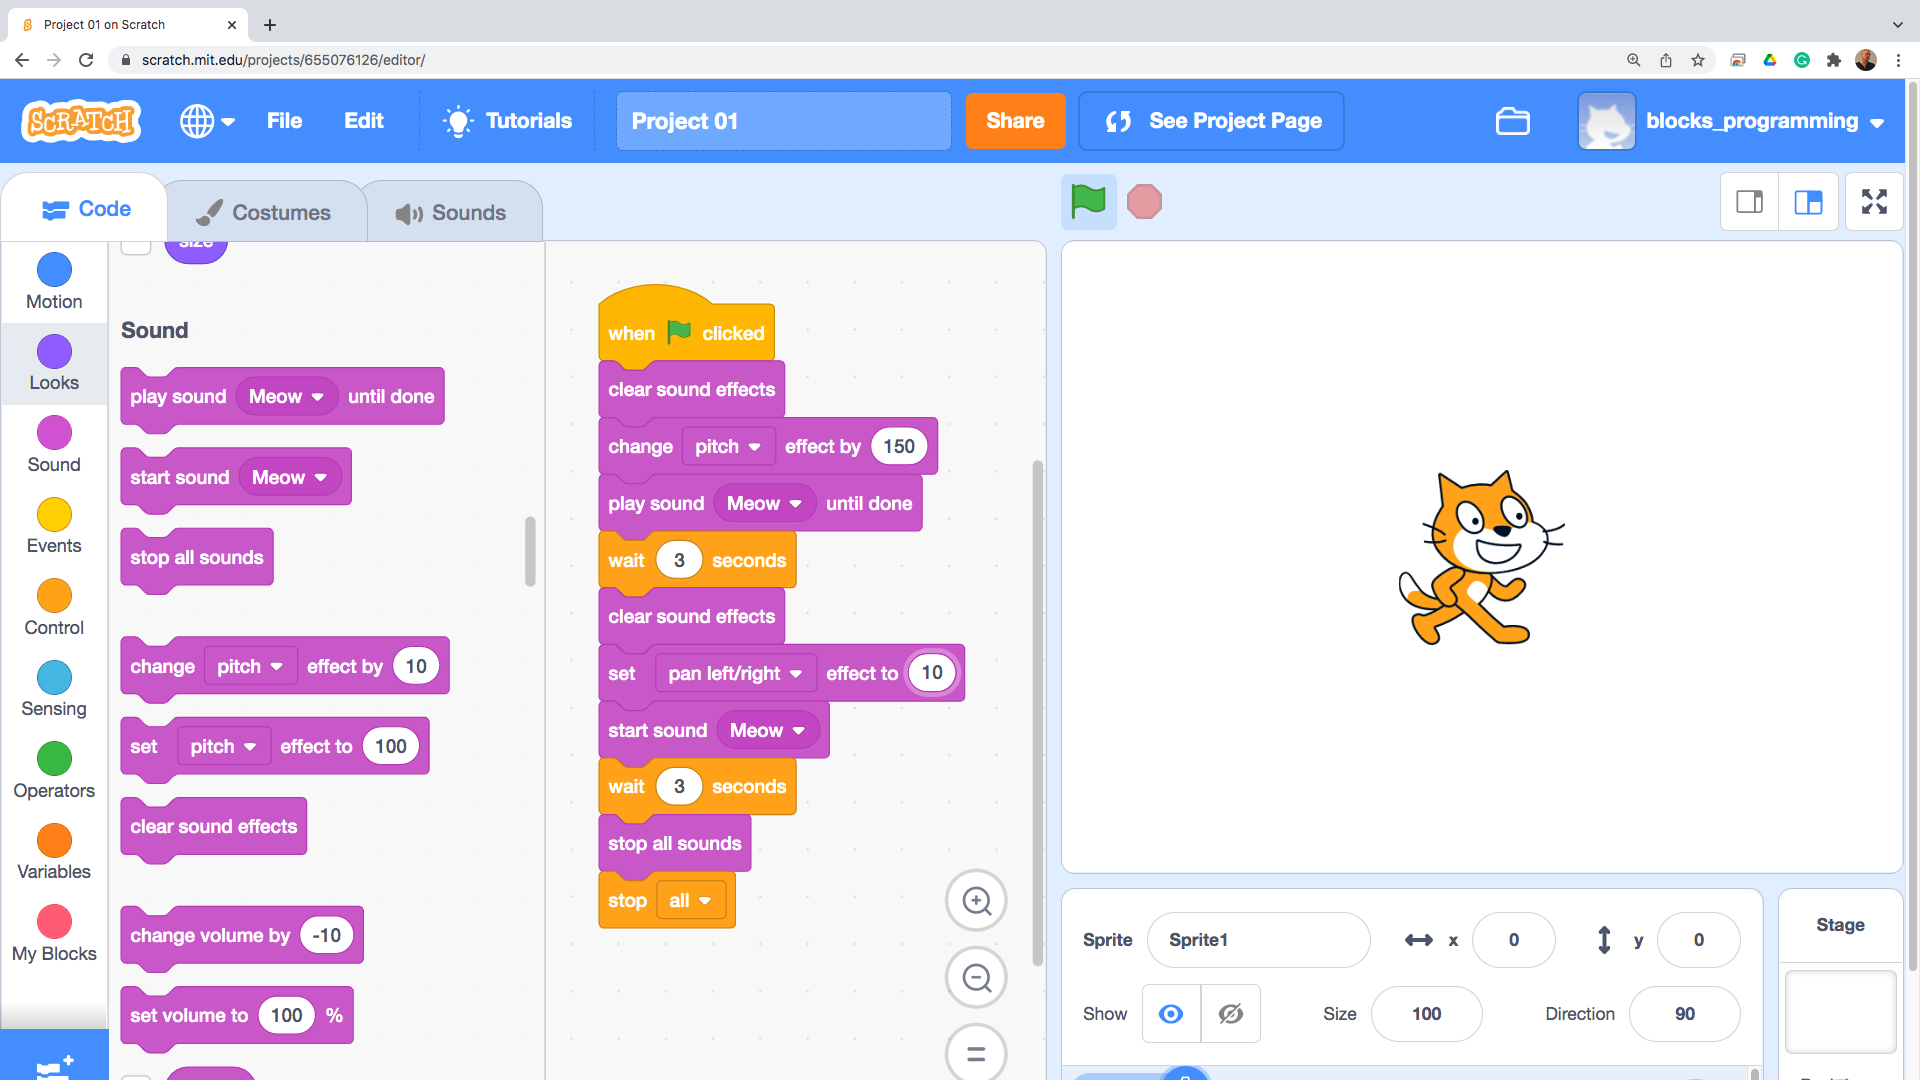
\includegraphics[width=1.0\linewidth,height=0.5\linewidth]{fig020027.png}
  \caption{Характеристики на звука}
\label{fig020027}
\end{figure}

За постигането на една по-богата звукова картина, силата на различните звуци може да се управлява с две блокчета (Фиг. \ref{fig020028}). Първото контролира силата на звука по абсолютна стойност, а второто като проценти. 

\begin{figure}[H]
  \centering
  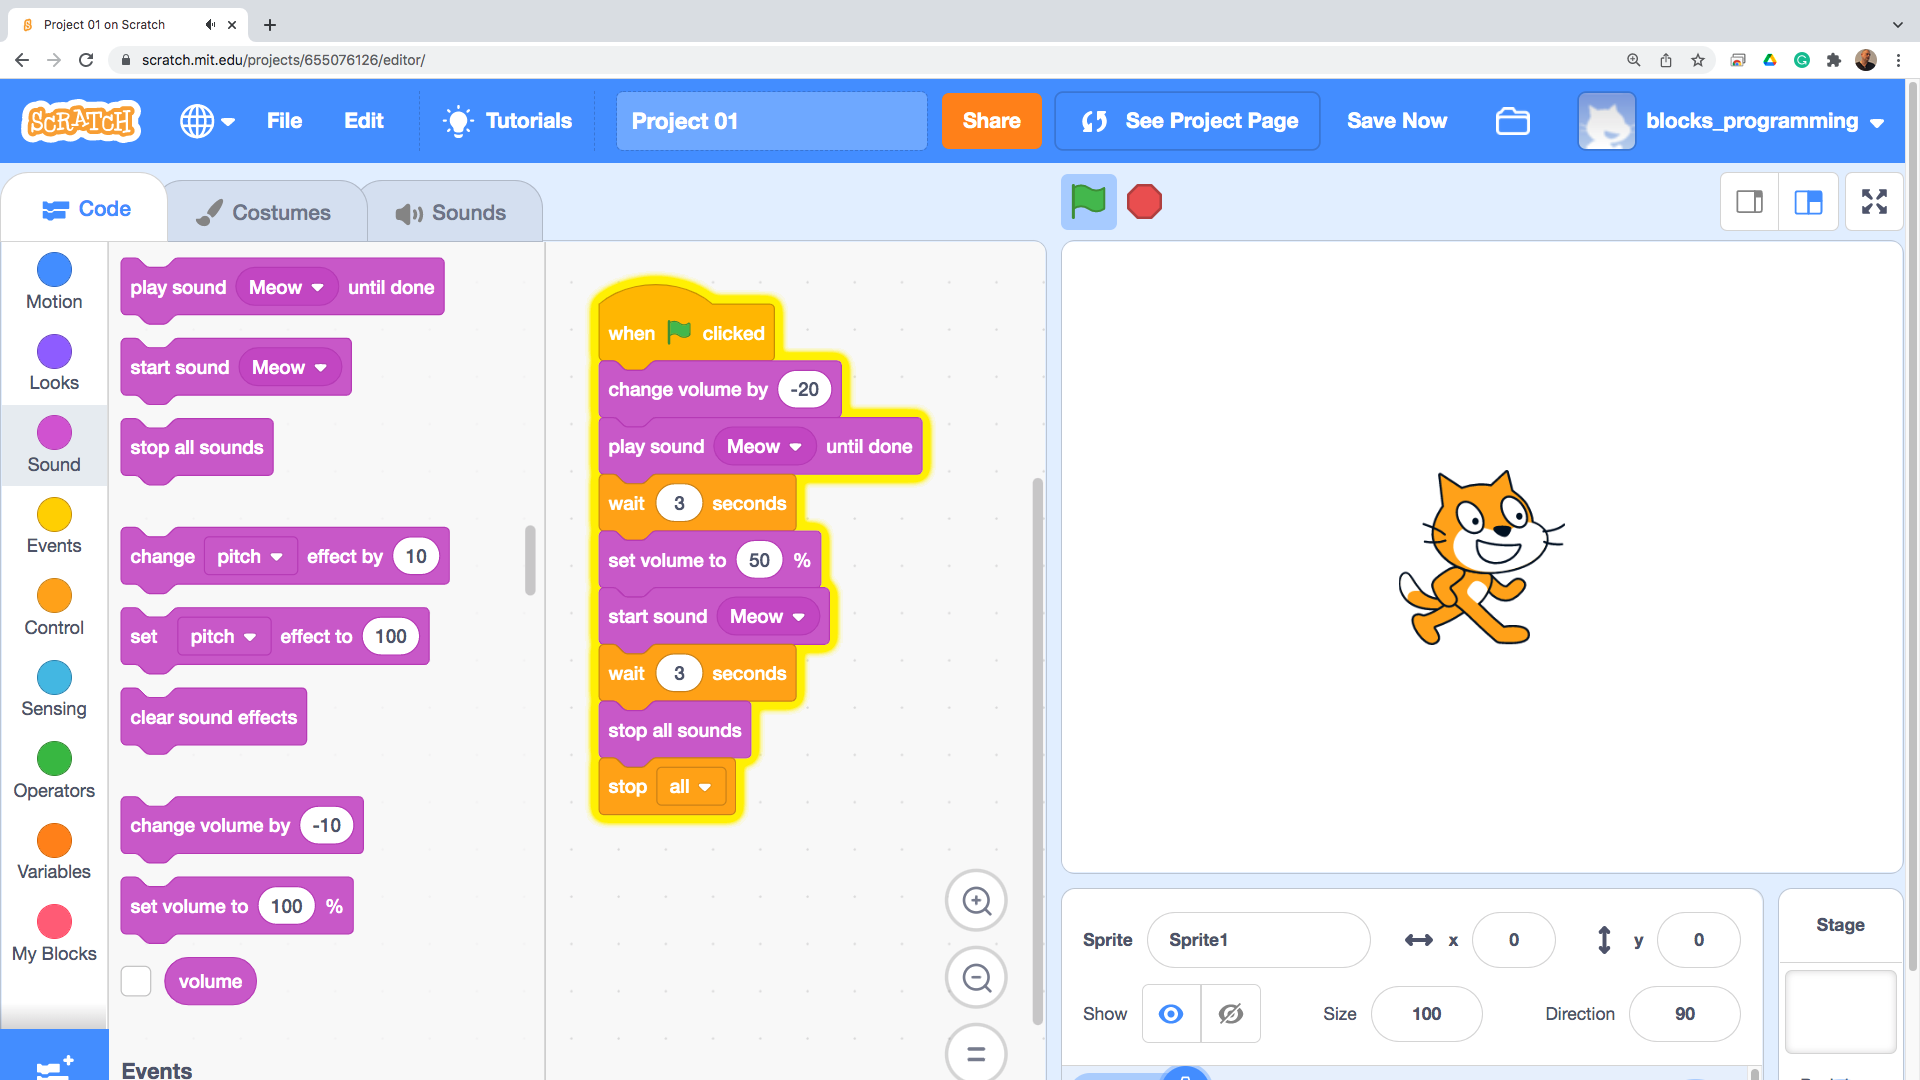
\includegraphics[width=1.0\linewidth,height=0.5\linewidth]{fig020028.png}
  \caption{Сила на звука}
\label{fig020028}
\end{figure}

Оранжевата група блокчета са предназначени за възникване на събития. Събитията са инструмент за изпълнение на инструкции, когато няма ясна престава за момента в който програмните инструкции трябва да се изпълнят. Такова събитие е натискане на бутон по клавиатурата от страна на потребителя (Фиг. \ref{fig020029}).

\begin{figure}[H]
  \centering
  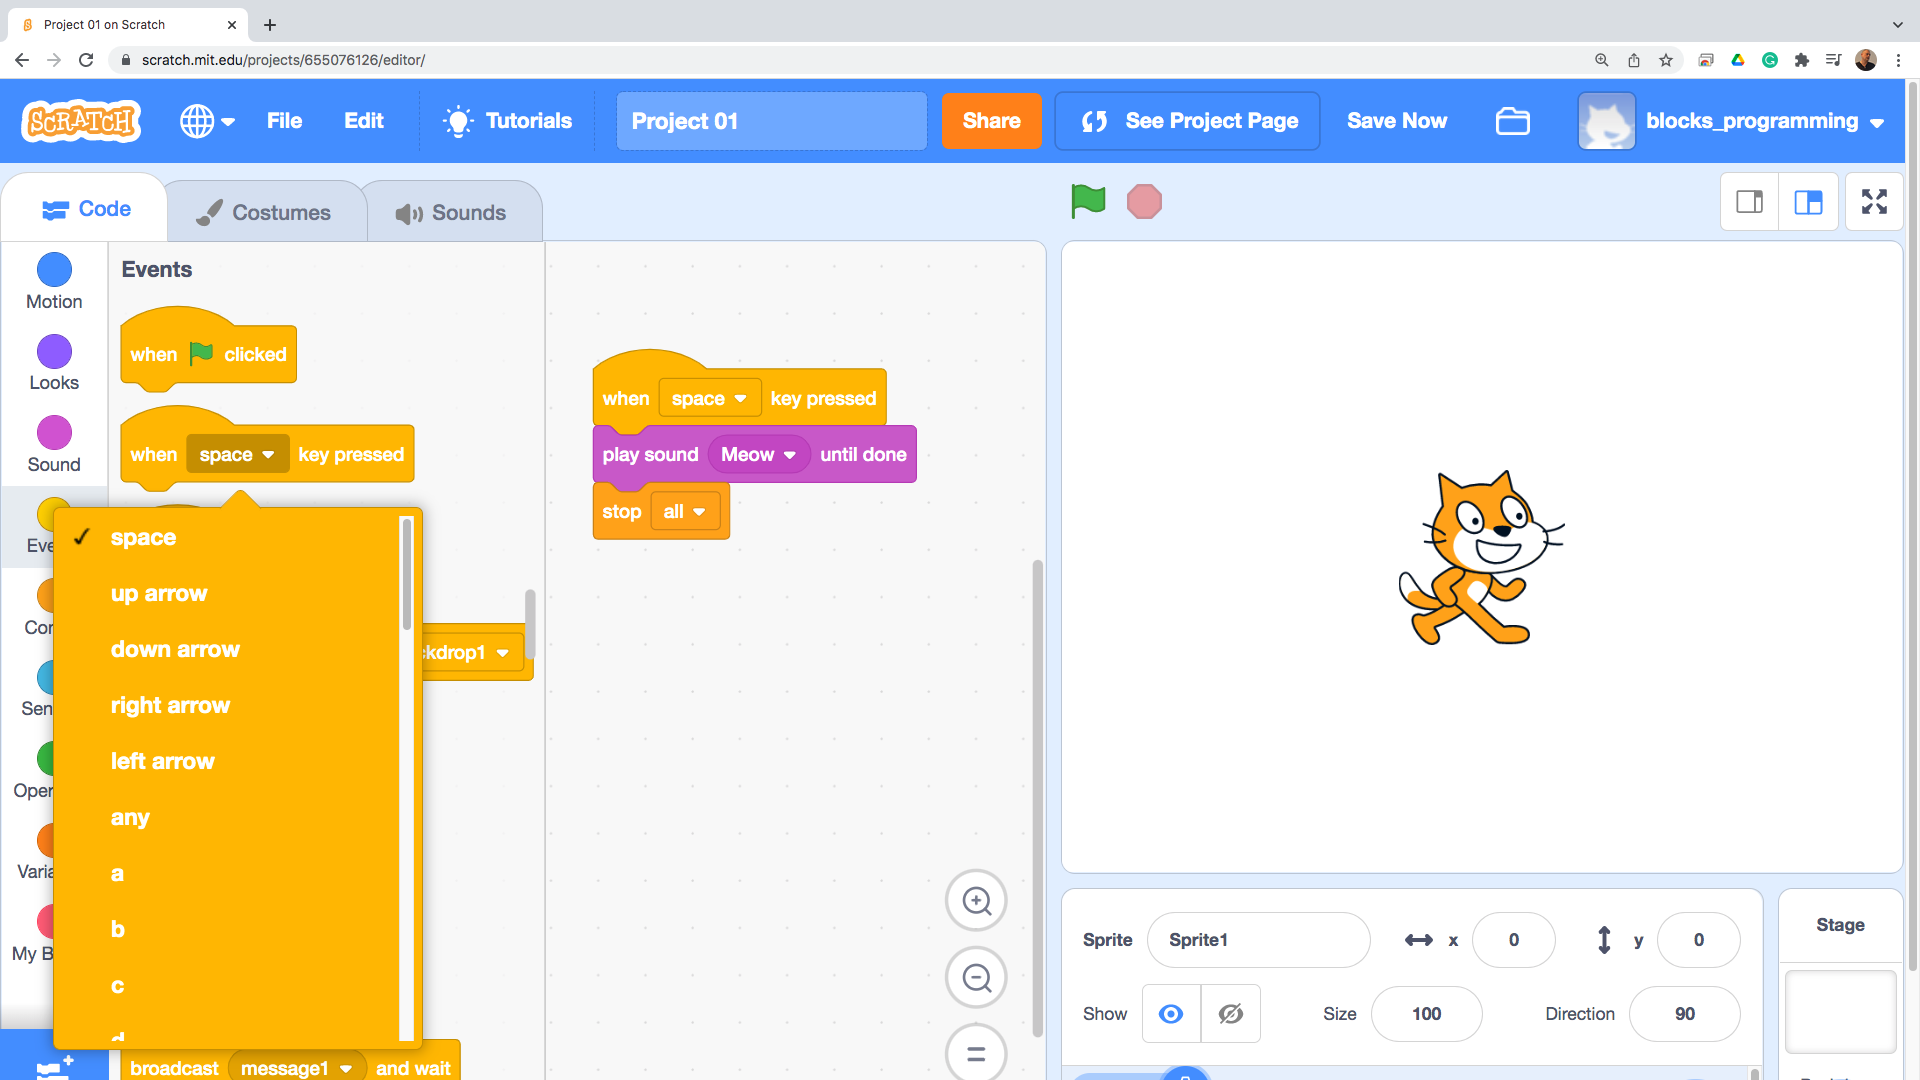
\includegraphics[width=1.0\linewidth,height=0.5\linewidth]{fig020029.png}
  \caption{Събитие за натискане на клавиш}
\label{fig020029}
\end{figure}

Кликването с мишката върху определен спрайт също може да бъде обработено с помощта на подходящо блокче (Фиг. \ref{fig020030}).

\begin{figure}[H]
  \centering
  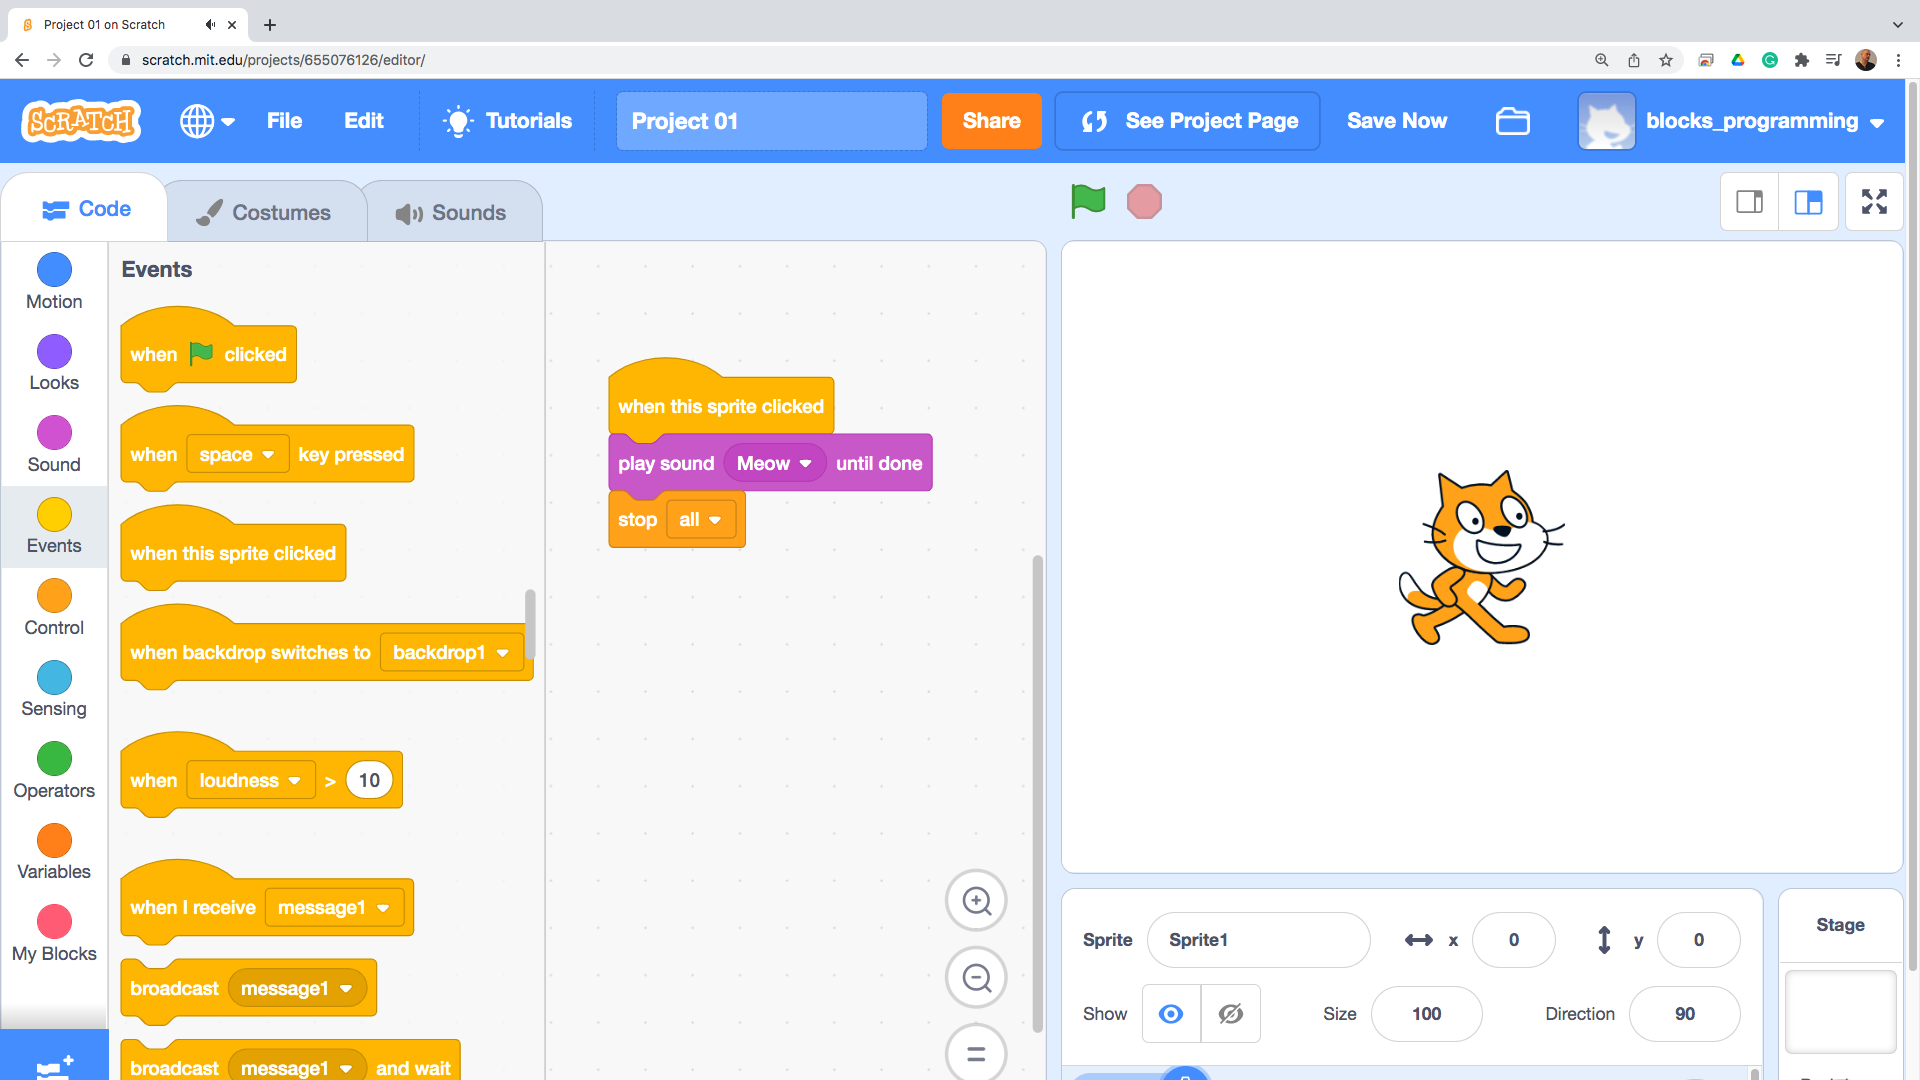
\includegraphics[width=1.0\linewidth,height=0.5\linewidth]{fig020030.png}
  \caption{Събитие за кликане с мишката}
\label{fig020030}
\end{figure}

Смяната на фона също може да предизвика обработване на събитие. За тази цел има предвидено блокче (Фиг. \ref{fig020031}).

\begin{figure}[H]
  \centering
  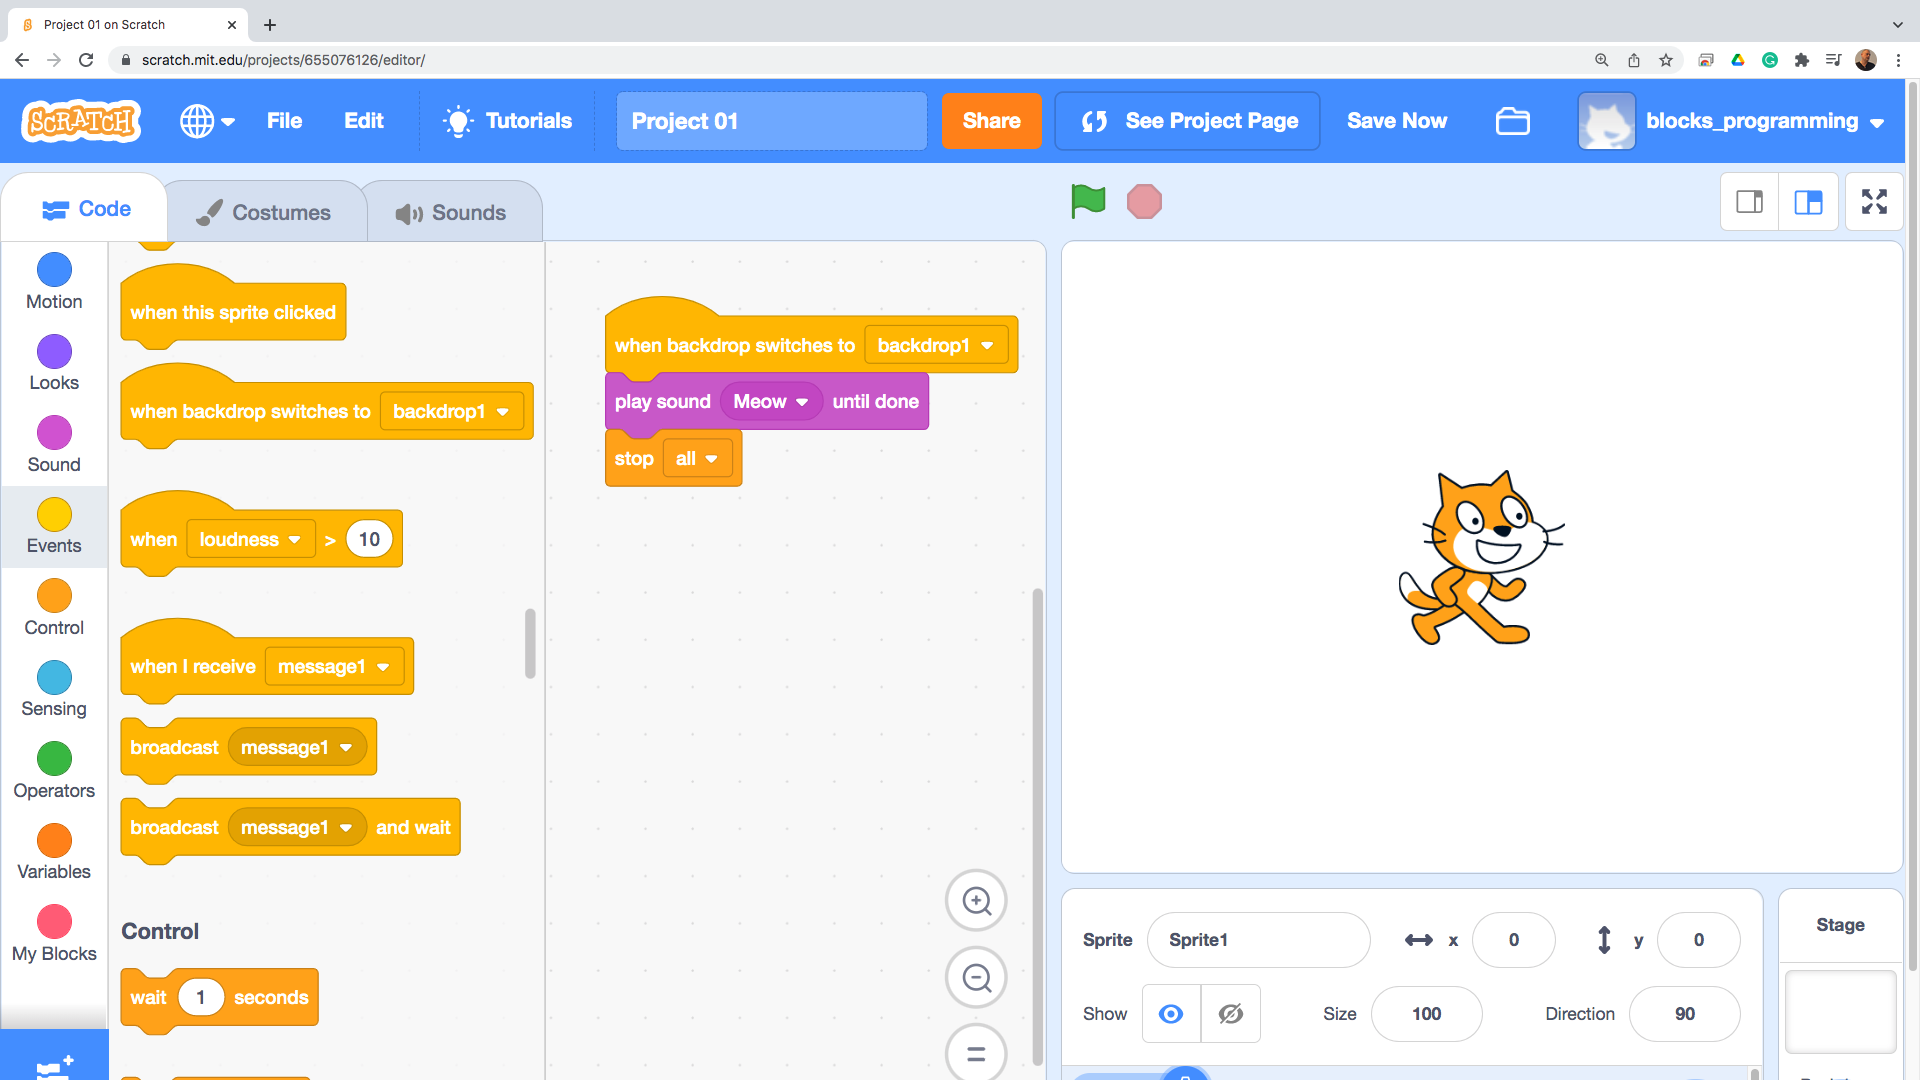
\includegraphics[width=1.0\linewidth,height=0.5\linewidth]{fig020031.png}
  \caption{Събитие за смяна на фона}
\label{fig020031}
\end{figure}

Събитие може да бъде прихванато след изтичане на определено време към таймер или достигане на определено ниво на звук (Фиг. \ref{fig020032}).

\begin{figure}[H]
  \centering
  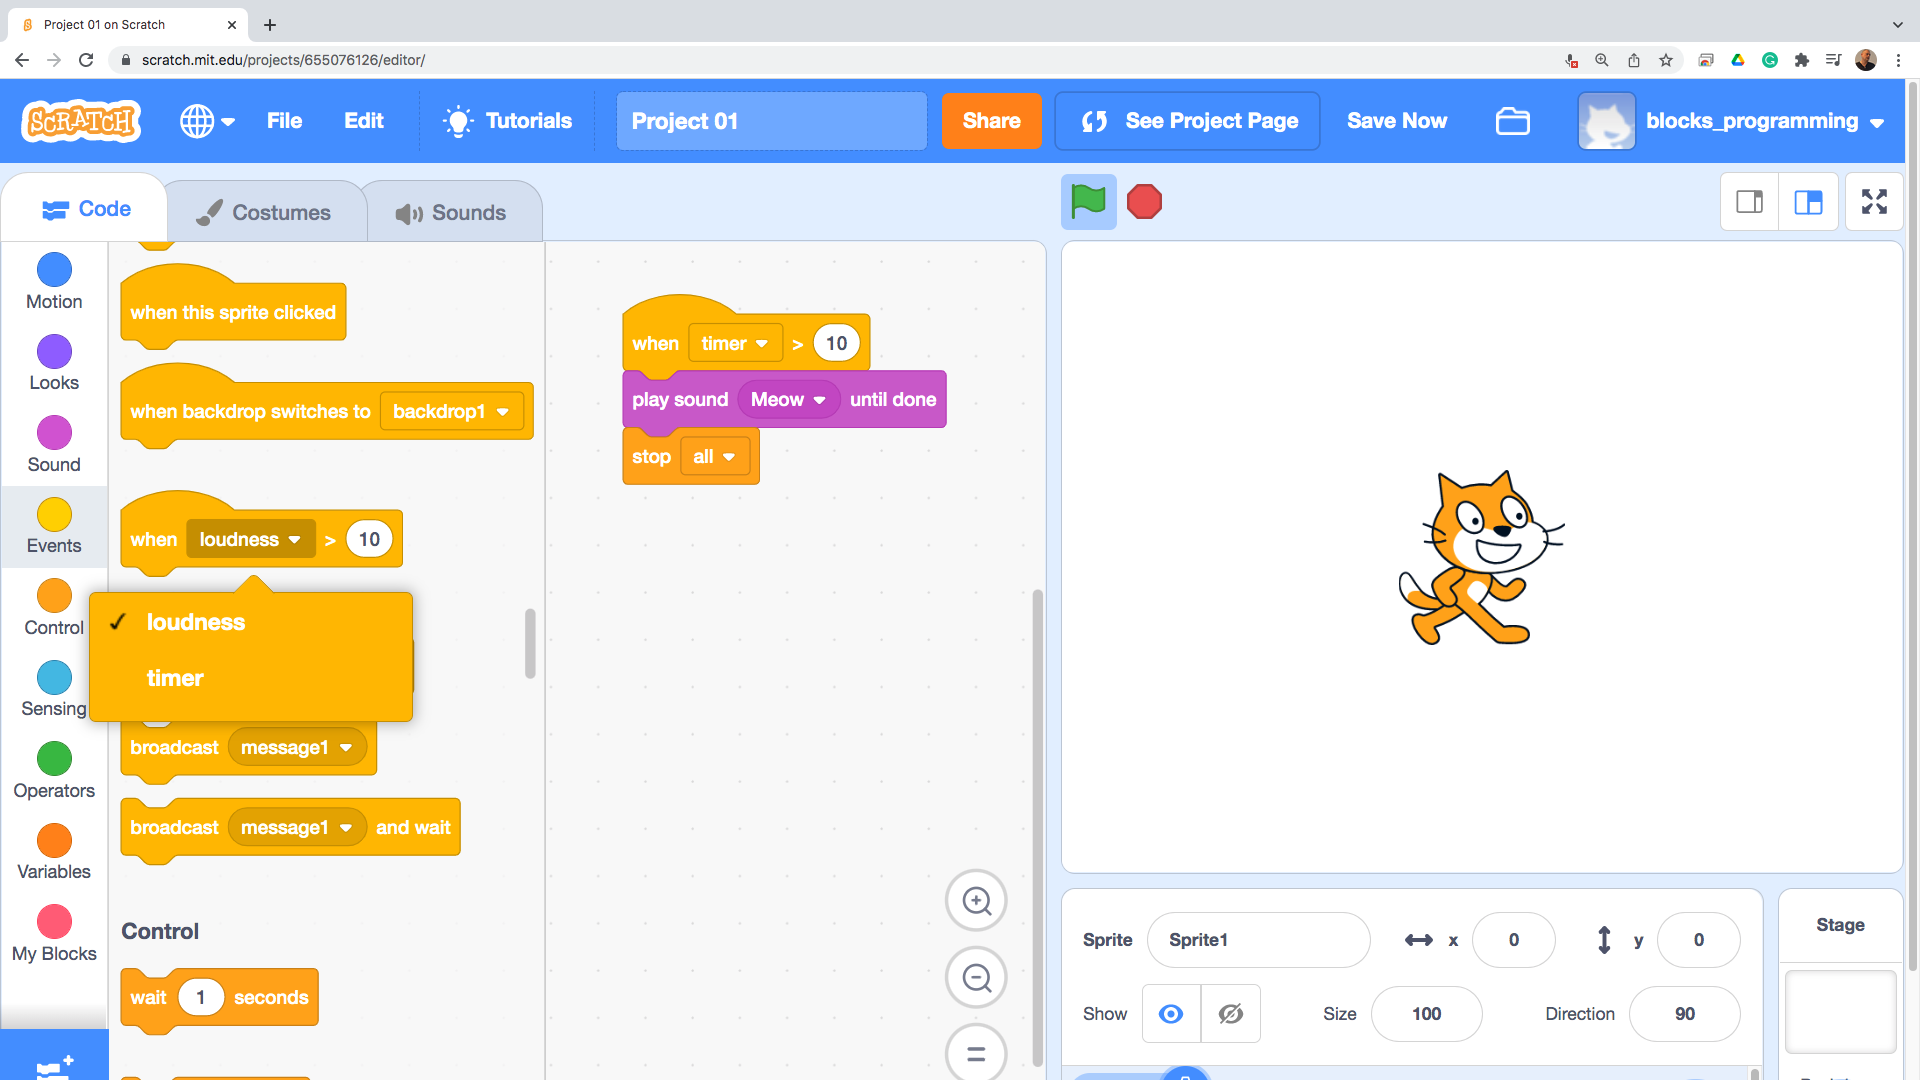
\includegraphics[width=1.0\linewidth,height=0.5\linewidth]{fig020032.png}
  \caption{Събитие от таймер или звук}
\label{fig020032}
\end{figure}

Работата със събития е свързана и с механизъм за предаване/получаване на съобщения. Един блок инструкции може да разпространи предварително дефинирано съобщение, а друг блок инструкции може да се абонира за получаването на точно този вид съобщение (Фиг. \ref{fig020033}).

\begin{figure}[H]
  \centering
  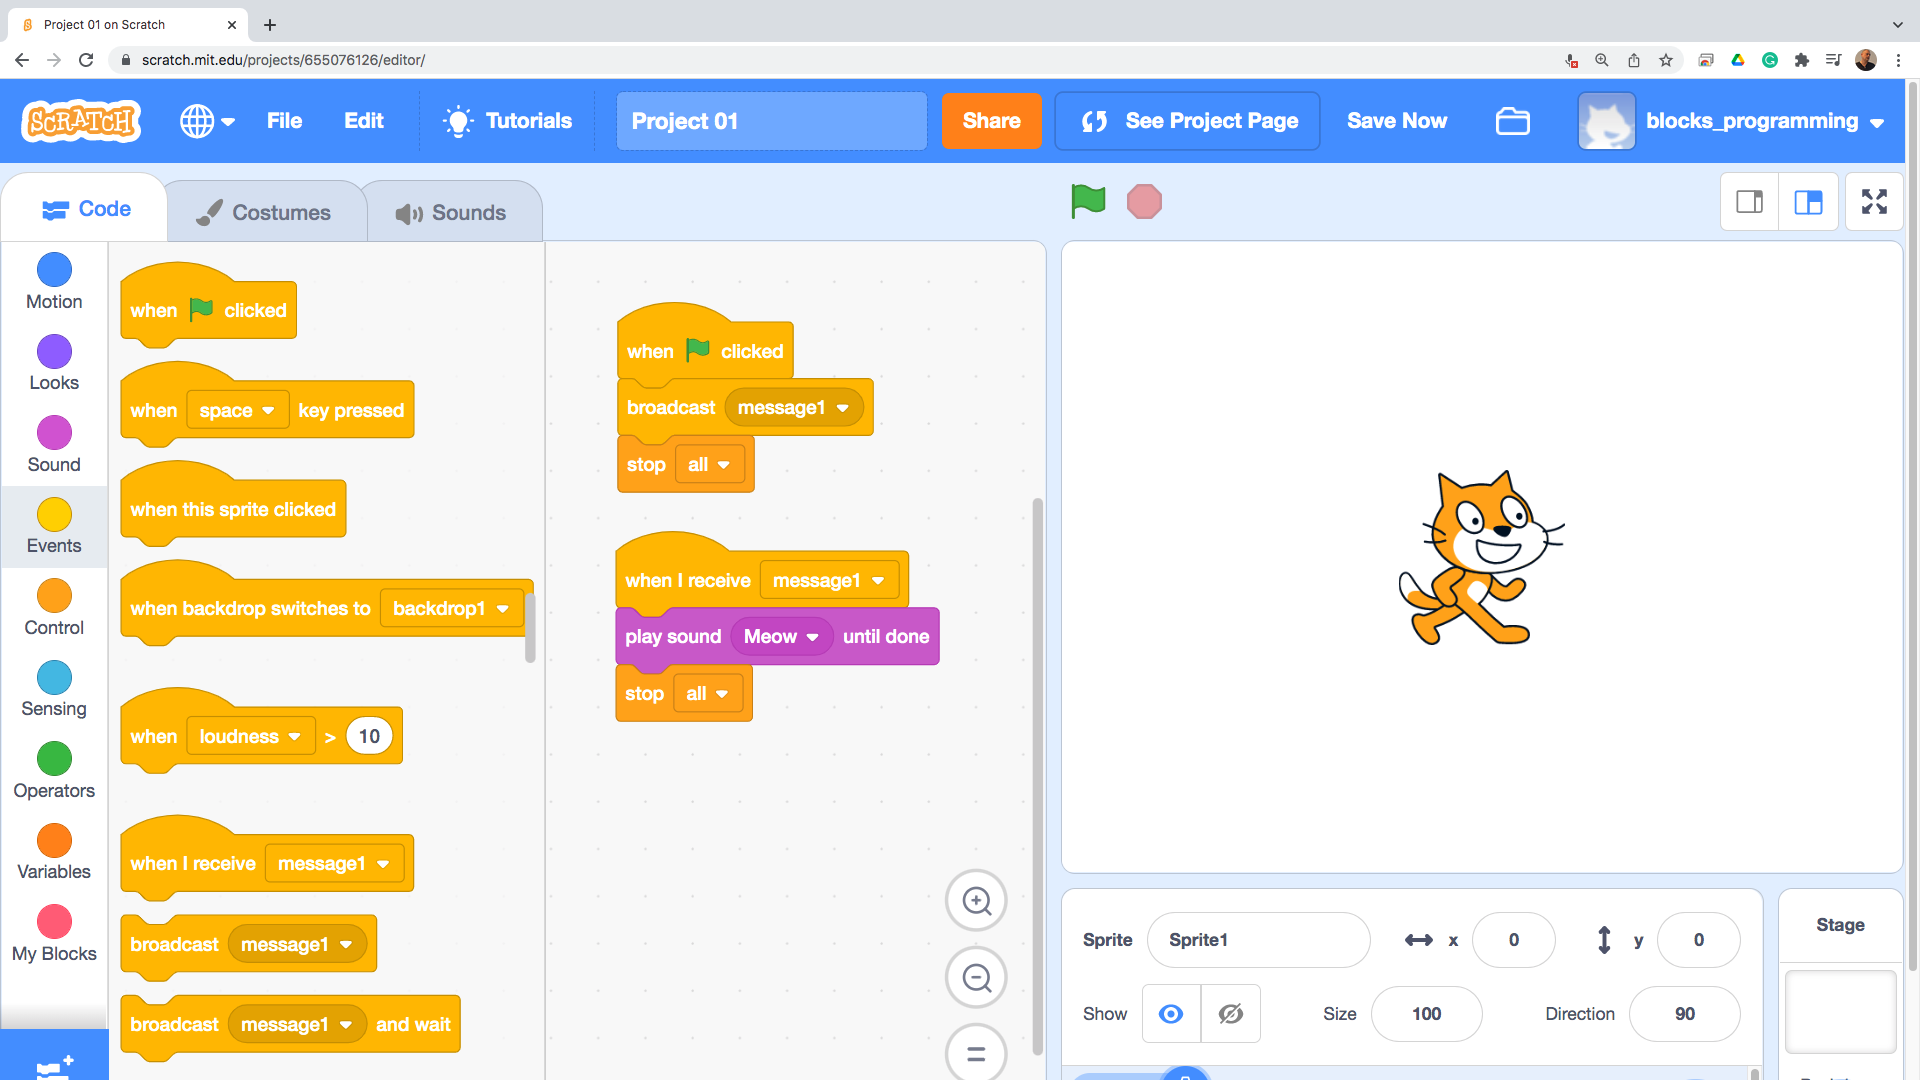
\includegraphics[width=1.0\linewidth,height=0.5\linewidth]{fig020033.png}
  \caption{Разпространяване и получаване на съобщения}
\label{fig020033}
\end{figure}

Тъй като работата с механизма за съобщения може да изисква синхронизация, то има отделно блокче, което разпространява съобщението и изчаква извършването на действията от прихващането му (Фиг. \ref{fig020034}). Програмистът може да създава различни съобщения, които да бъдат изпращани в различни ситуации. 

\begin{figure}[H]
  \centering
  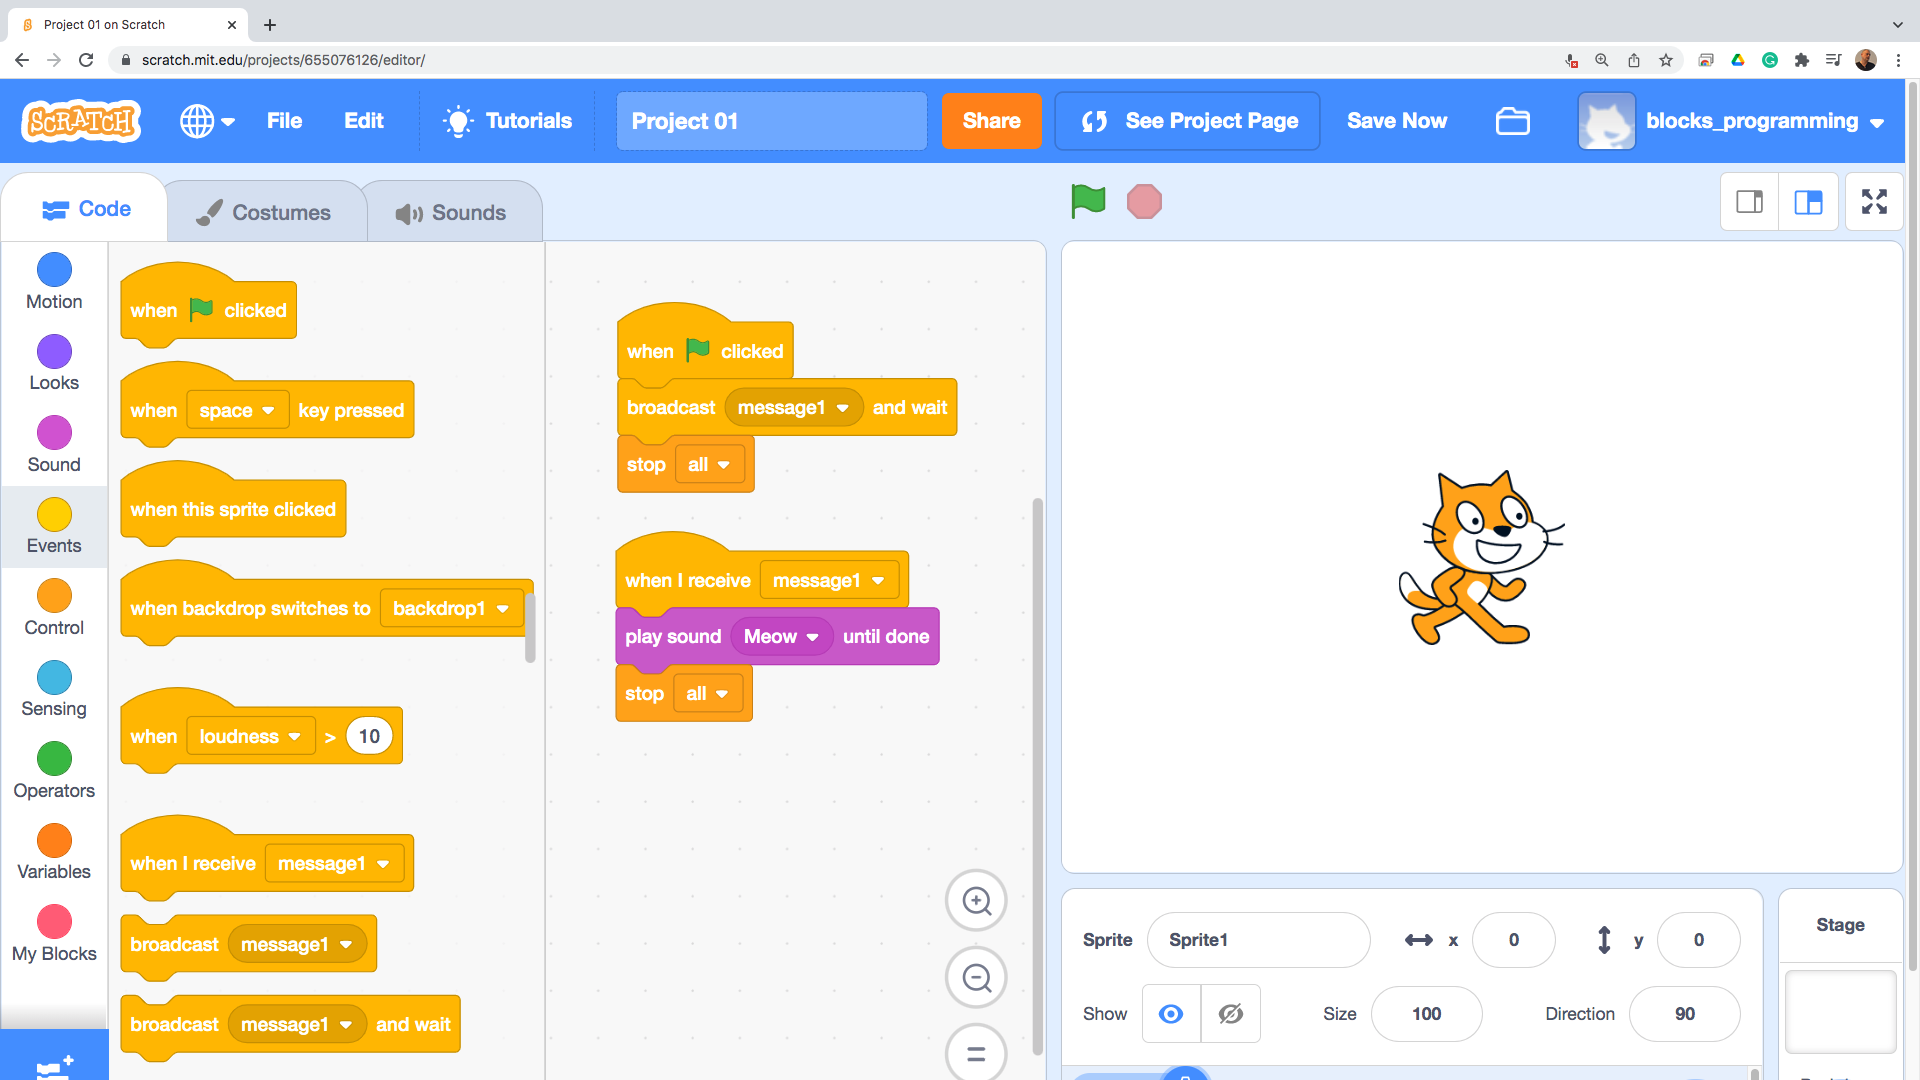
\includegraphics[width=1.0\linewidth,height=0.5\linewidth]{fig020034.png}
  \caption{Разпространяване на съобщение с изчакване}
\label{fig020034}
\end{figure}

Най-важните, а и най-полезните блокчета са организирани в групата на тъмно оранжевите. Това са блокчета, които определят по коя пътека на изпълнение ще се поеме, спрямо възможните избори за изпълнение на инструкции. Когато желанието е определено действие да се изпълни многократно, при зададен брой повторения, за тази цел има конкретно блокче (Фиг. \ref{fig020035}). В програмирането, многократните повторения се осъществяват с помощта на конструкции за цикъл, какъвто е случаят и с това блокче за повторения.

\begin{figure}[H]
  \centering
  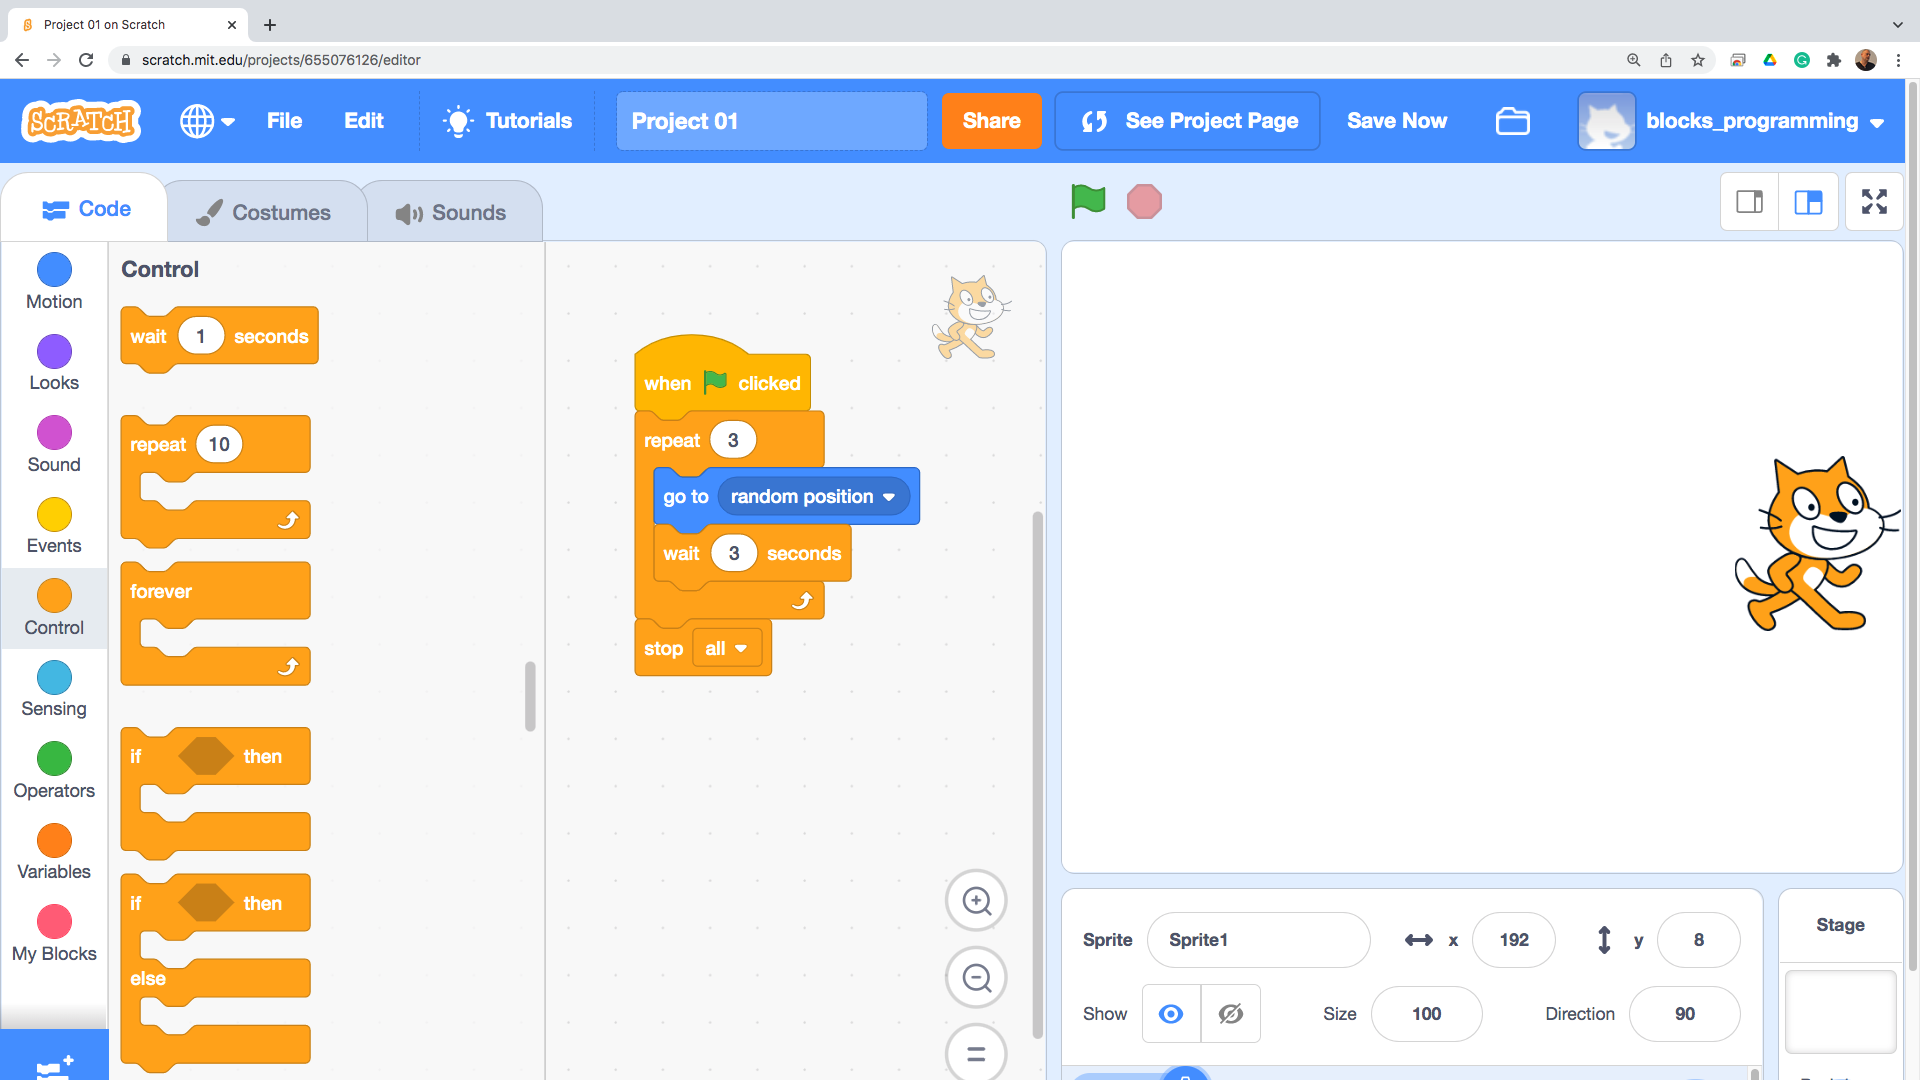
\includegraphics[width=1.0\linewidth,height=0.5\linewidth]{fig020035.png}
  \caption{Фиксиран брой повторения}
\label{fig020035}
\end{figure}

Думичката repeat от английски означава повтори. Числото в блокчето определя колко на брой повторения да бъдат изпълнени, а в слота на блочето се поставят инструкциите, които да бъдат повтаряни. В този пример, котето се премества на случайно избрани координати, след което следва изчакване от предварително определен брой секунди. В много редки ситуации има нужда от безкрайно повтарящ се цикъл, за което е предвидено отделно блокче (Фиг. \ref{fig020036}).

\begin{figure}[H]
  \centering
  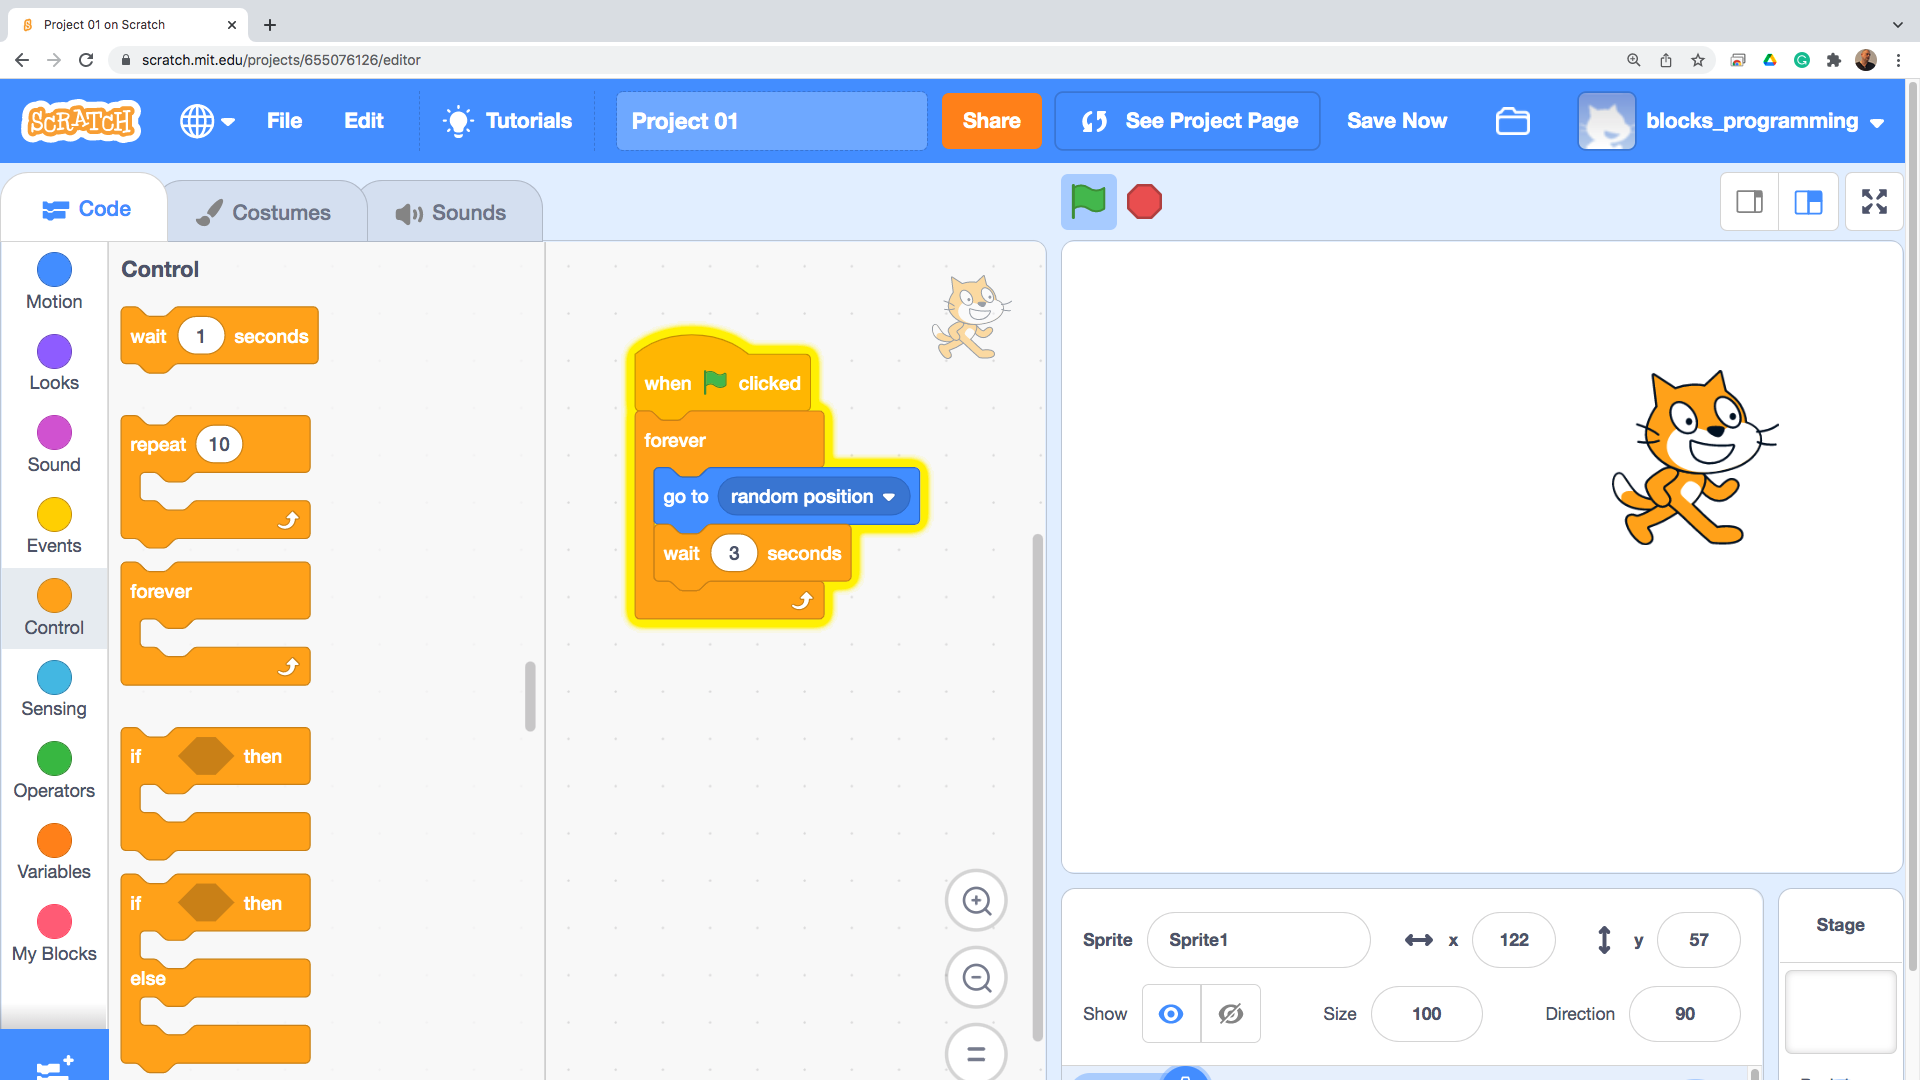
\includegraphics[width=1.0\linewidth,height=0.5\linewidth]{fig020036.png}
  \caption{Безкрайни повторения}
\label{fig020036}
\end{figure}

Следващото блокче е едно от най-важните блокчета в програмирането. То се нарича блокче за изпълнение при условие (Фиг. \ref{fig020037}) или условен преход. Съдържанието на блокчето се изпълнява само, ако условието в заглавната му част се изпълнява.

\begin{figure}[H]
  \centering
  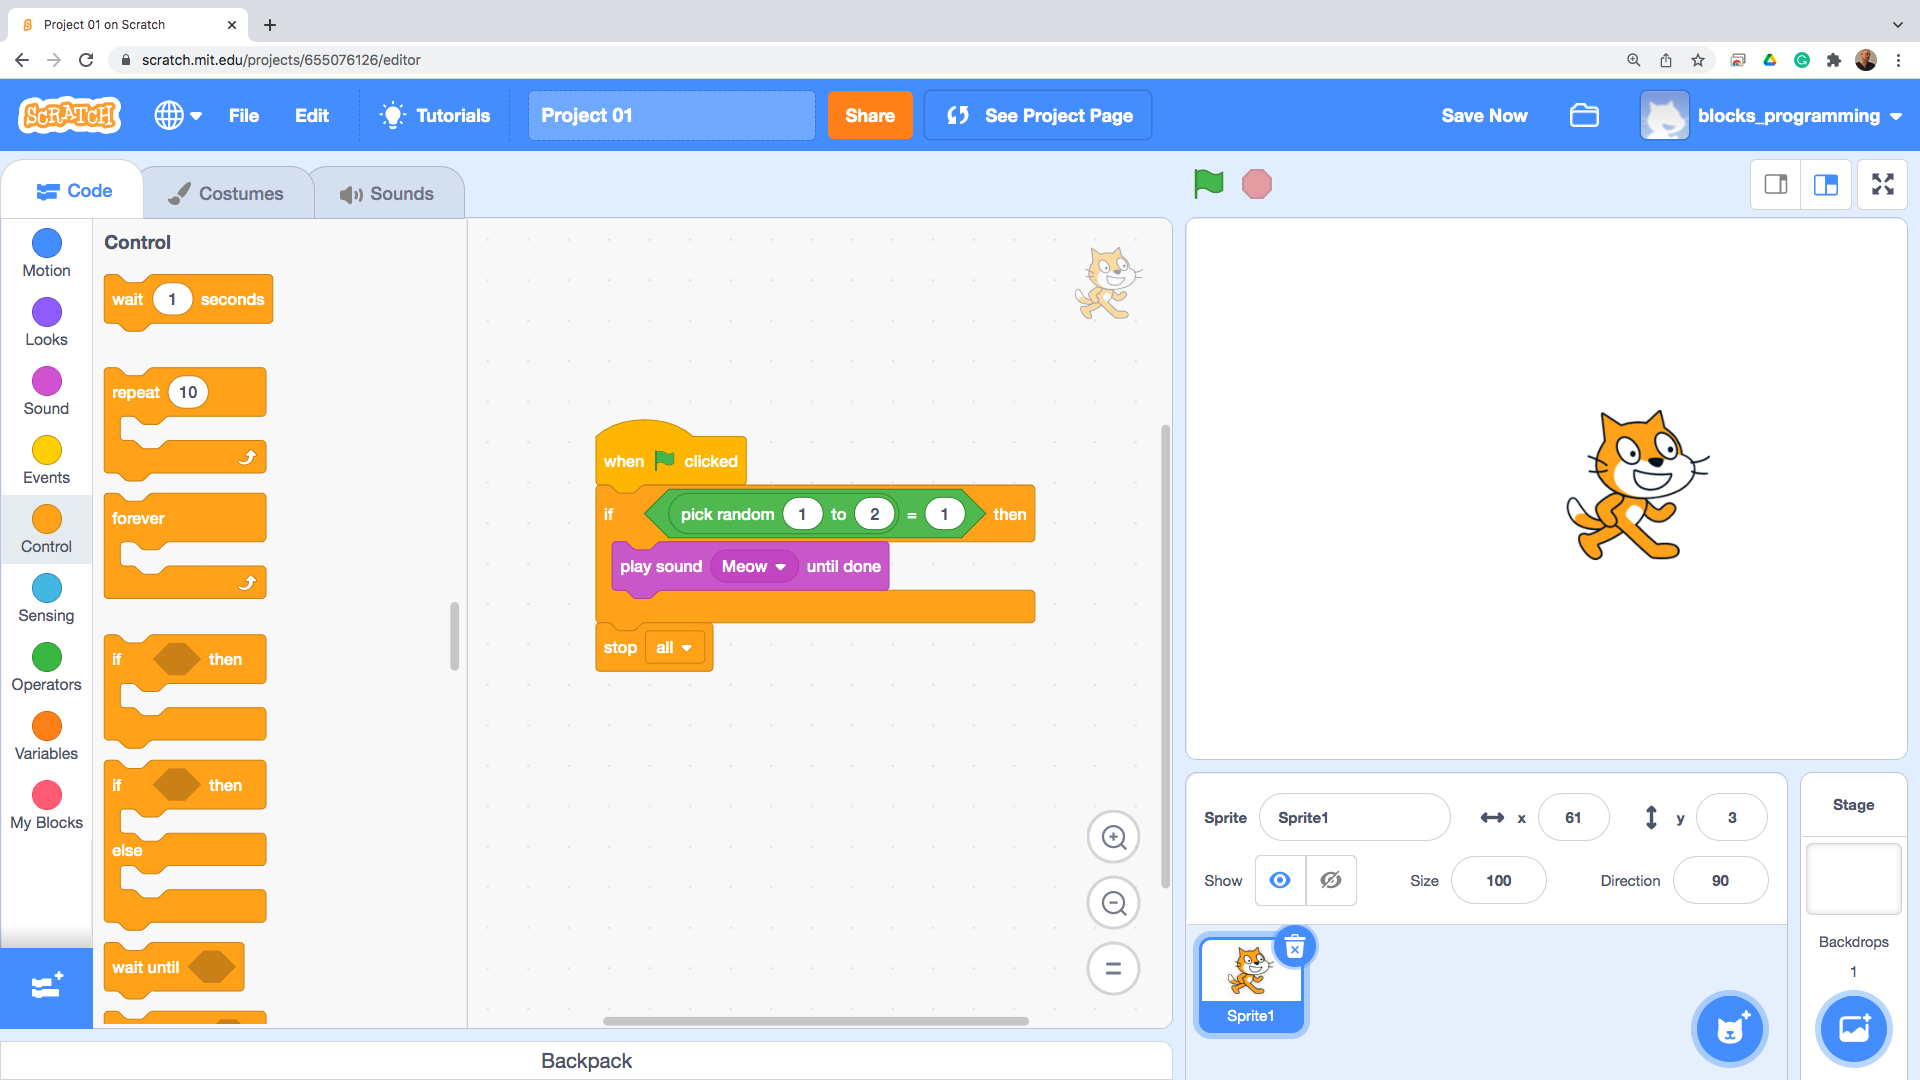
\includegraphics[width=1.0\linewidth,height=0.5\linewidth]{fig020037.png}
  \caption{Изпълнение при условие}
\label{fig020037}
\end{figure}

Това тъмно оранжево блокче не може да се използва само. То винаги е в съчетание с поне едно зелено блокче, а понякога и с две, както е в настоящия пример. Част от зелените блокчета са неправилни шестоъгълници и са направени така, че да пасват в заглавната част на някои от тъмно оранжевите блокчета. Самото шестоъгълно блокче има овален слот в който се поместват някои от зелените овални блокчета. В примера е избрано зелено блокче, което изисква равенство към конкретно число, а за овалното блокче се ползва генератор на случайни числа, според предварително зададен интервал. Ако условието в заглавната част на блокчето за условен преход не бъде изпълнено, то тялото се пропуска и се преминава към следващите инструкции, след блочкето. Блокчето за условен преход има и вариант в който се предвиждат слотове за изпълнение и на двете възможности – вярно условие или невярно условие (Фиг. \ref{fig020038}). Ако условието е изпълнено, се изпълнява първият блок с инструкции. Ако условието не е изпълнено, се изпълнява вторият блок с инструкции.

\begin{figure}[H]
  \centering
  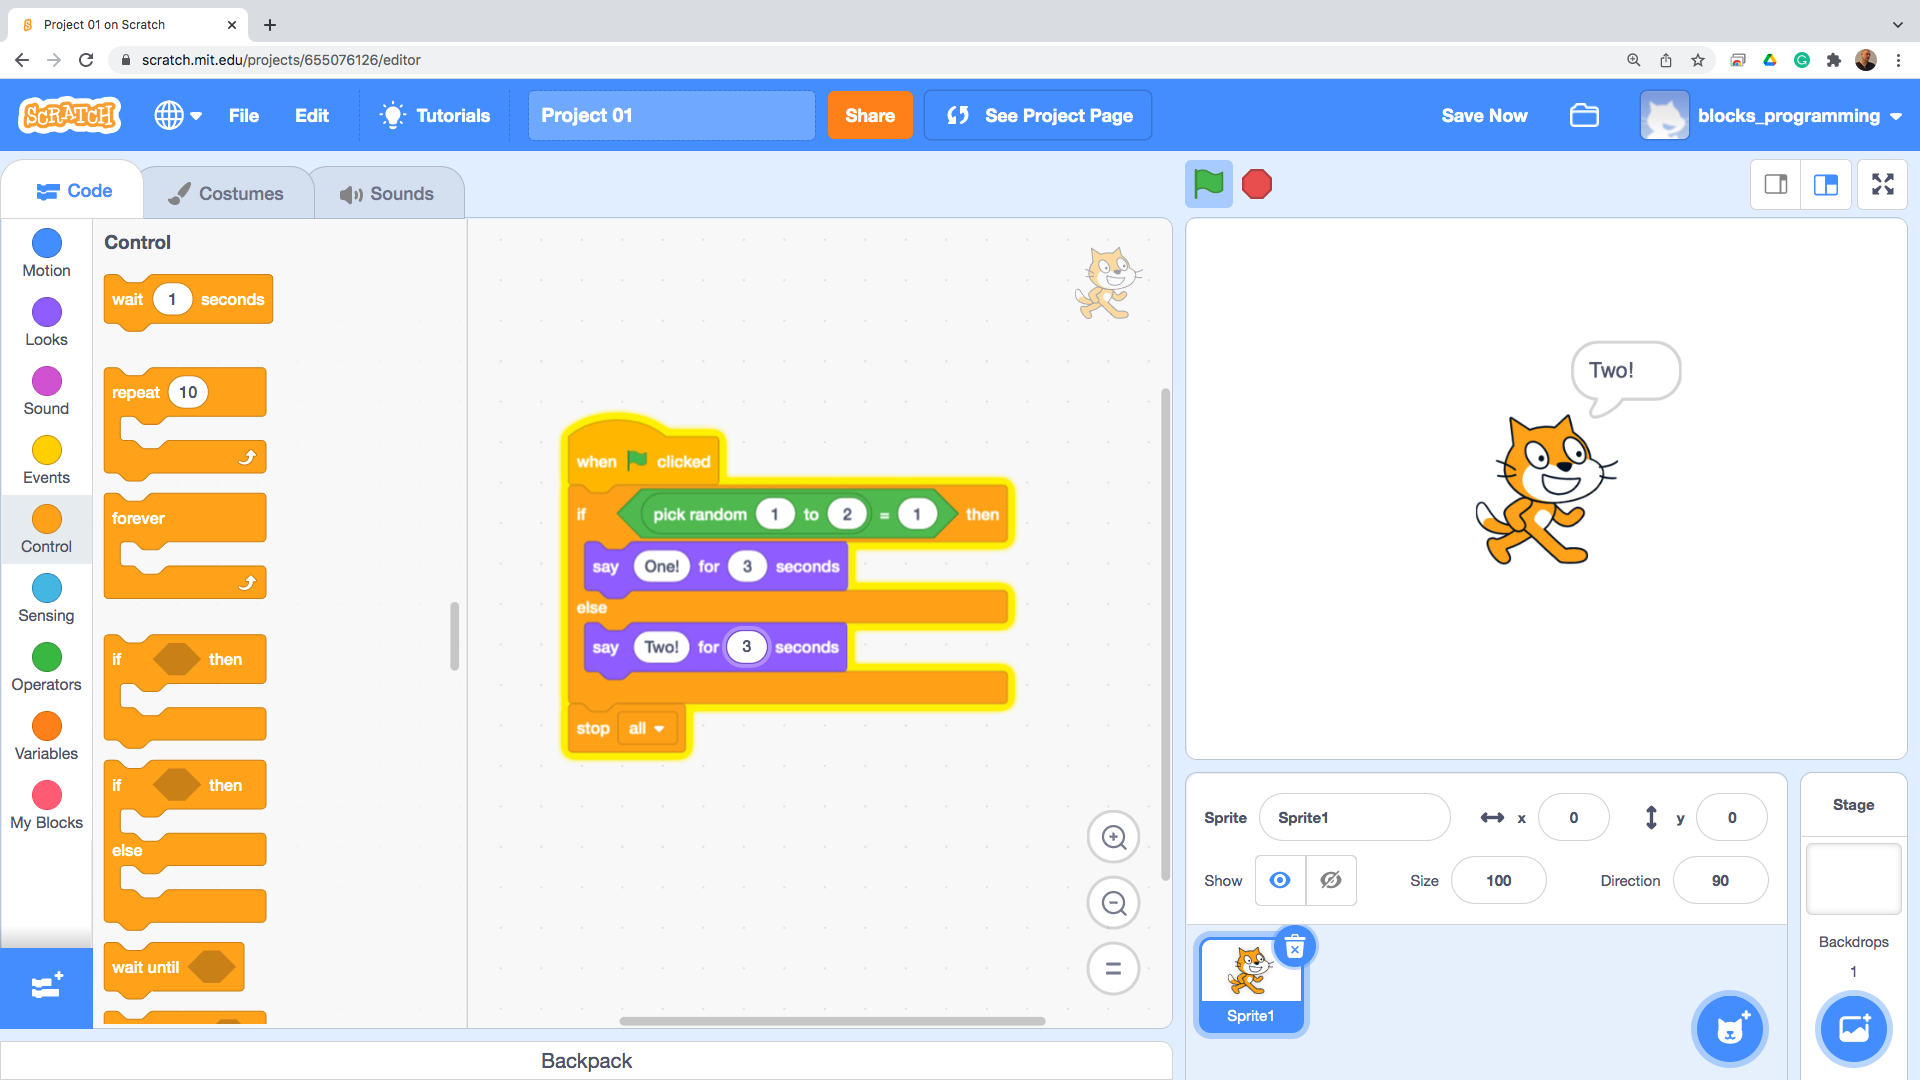
\includegraphics[width=1.0\linewidth,height=0.5\linewidth]{fig020038.png}
  \caption{Изпълнение при условие с алтернатива}
\label{fig020038}
\end{figure}

Следващото интересно блокче прави изчакване докато се случи определено събитие. В случая, събитието е спрайтът да бъде докоснат с мишката (Фиг. \ref{fig020039}). Случи ли се това докосване, изпълнението на програмата продължава към следващото блокче. Какво събитие се очаква е определено с допълнително блокче (светло синьо), което има формата на неправилен шестоъгълник.

\begin{figure}[H]
  \centering
  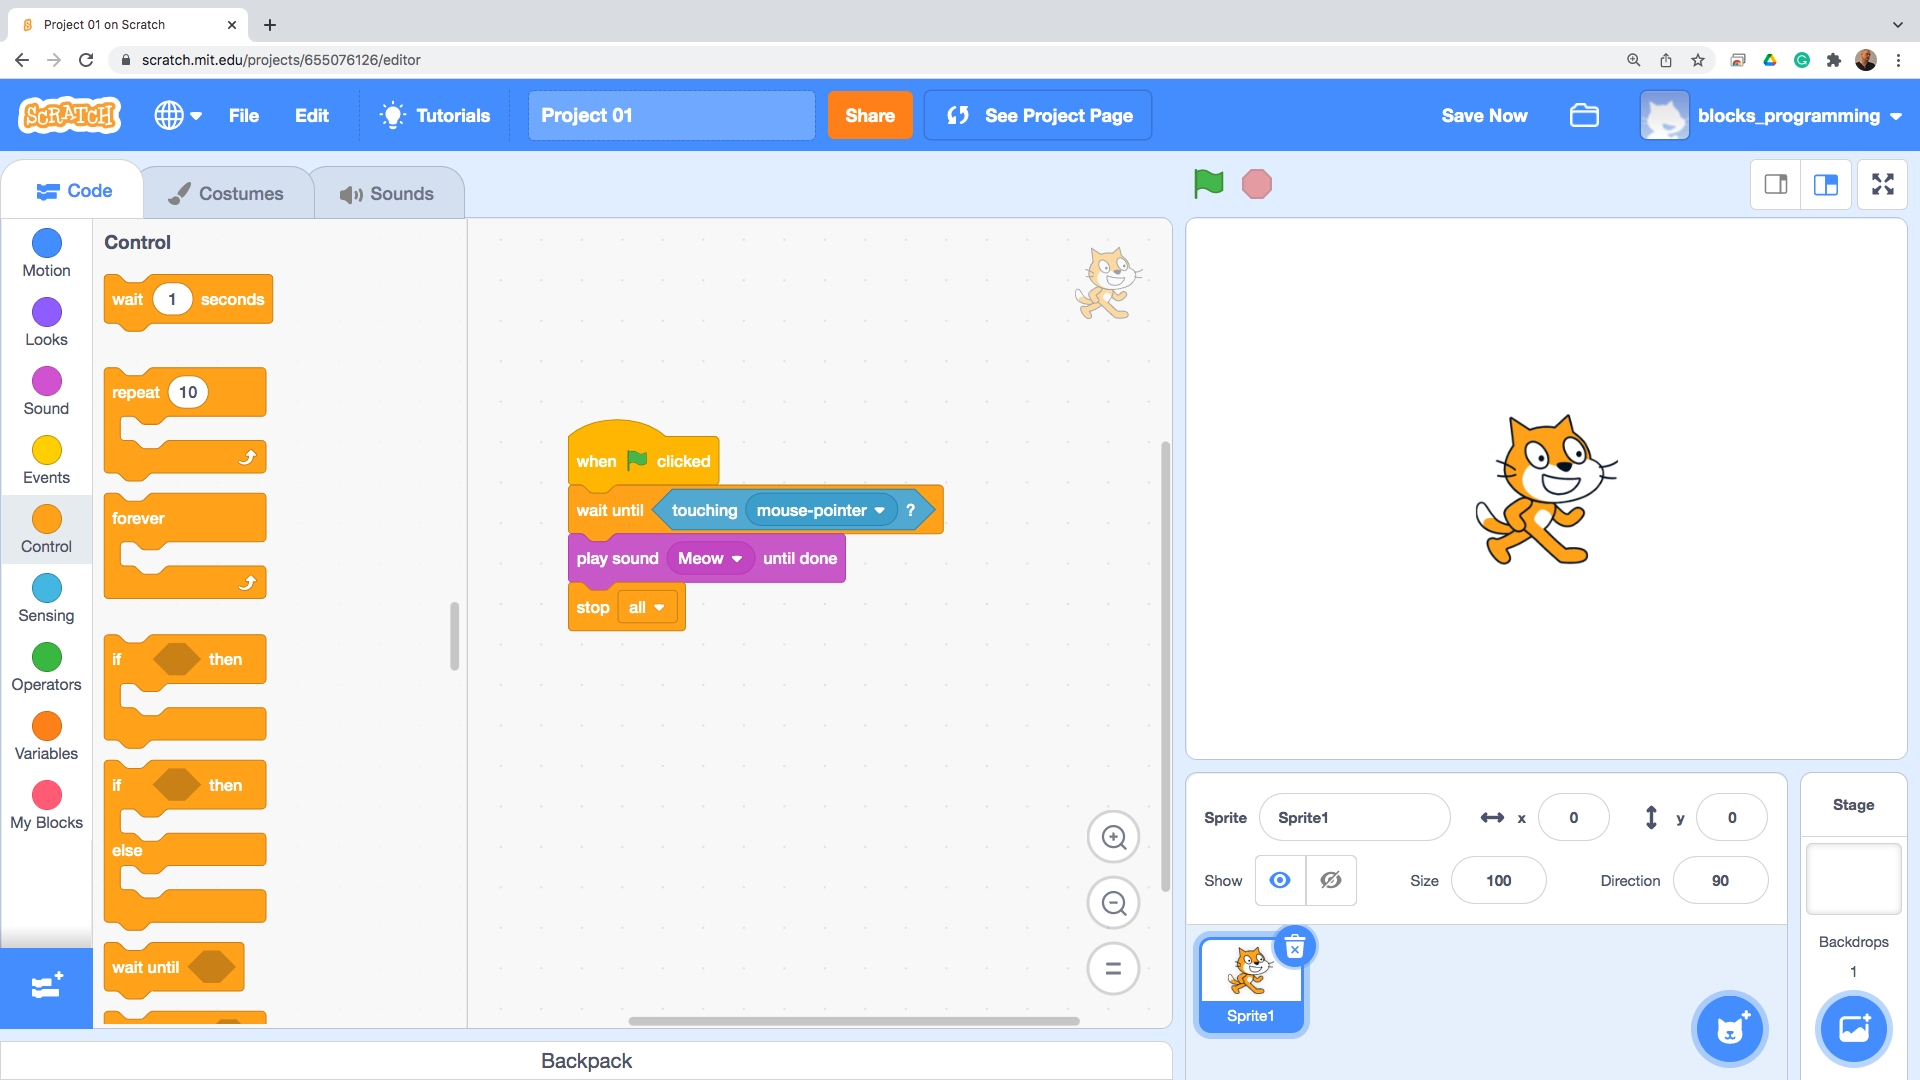
\includegraphics[width=1.0\linewidth,height=0.5\linewidth]{fig020039.png}
  \caption{Изчакване на условие}
\label{fig020039}
\end{figure}

Последните три блокчета в групата на тъмно оранжевите трябва да се демонстрират заедно (Фиг. \ref{fig020040}). Първото блокче задава нова верига от инструкции, когато определен спрай бъде клониран (копие на оригиналния спрайт). Второто блокче служи за клониране на текущия спрайт. А третото блокче служи за изтриване на текущия спрайт. 

\begin{figure}[H]
  \centering
  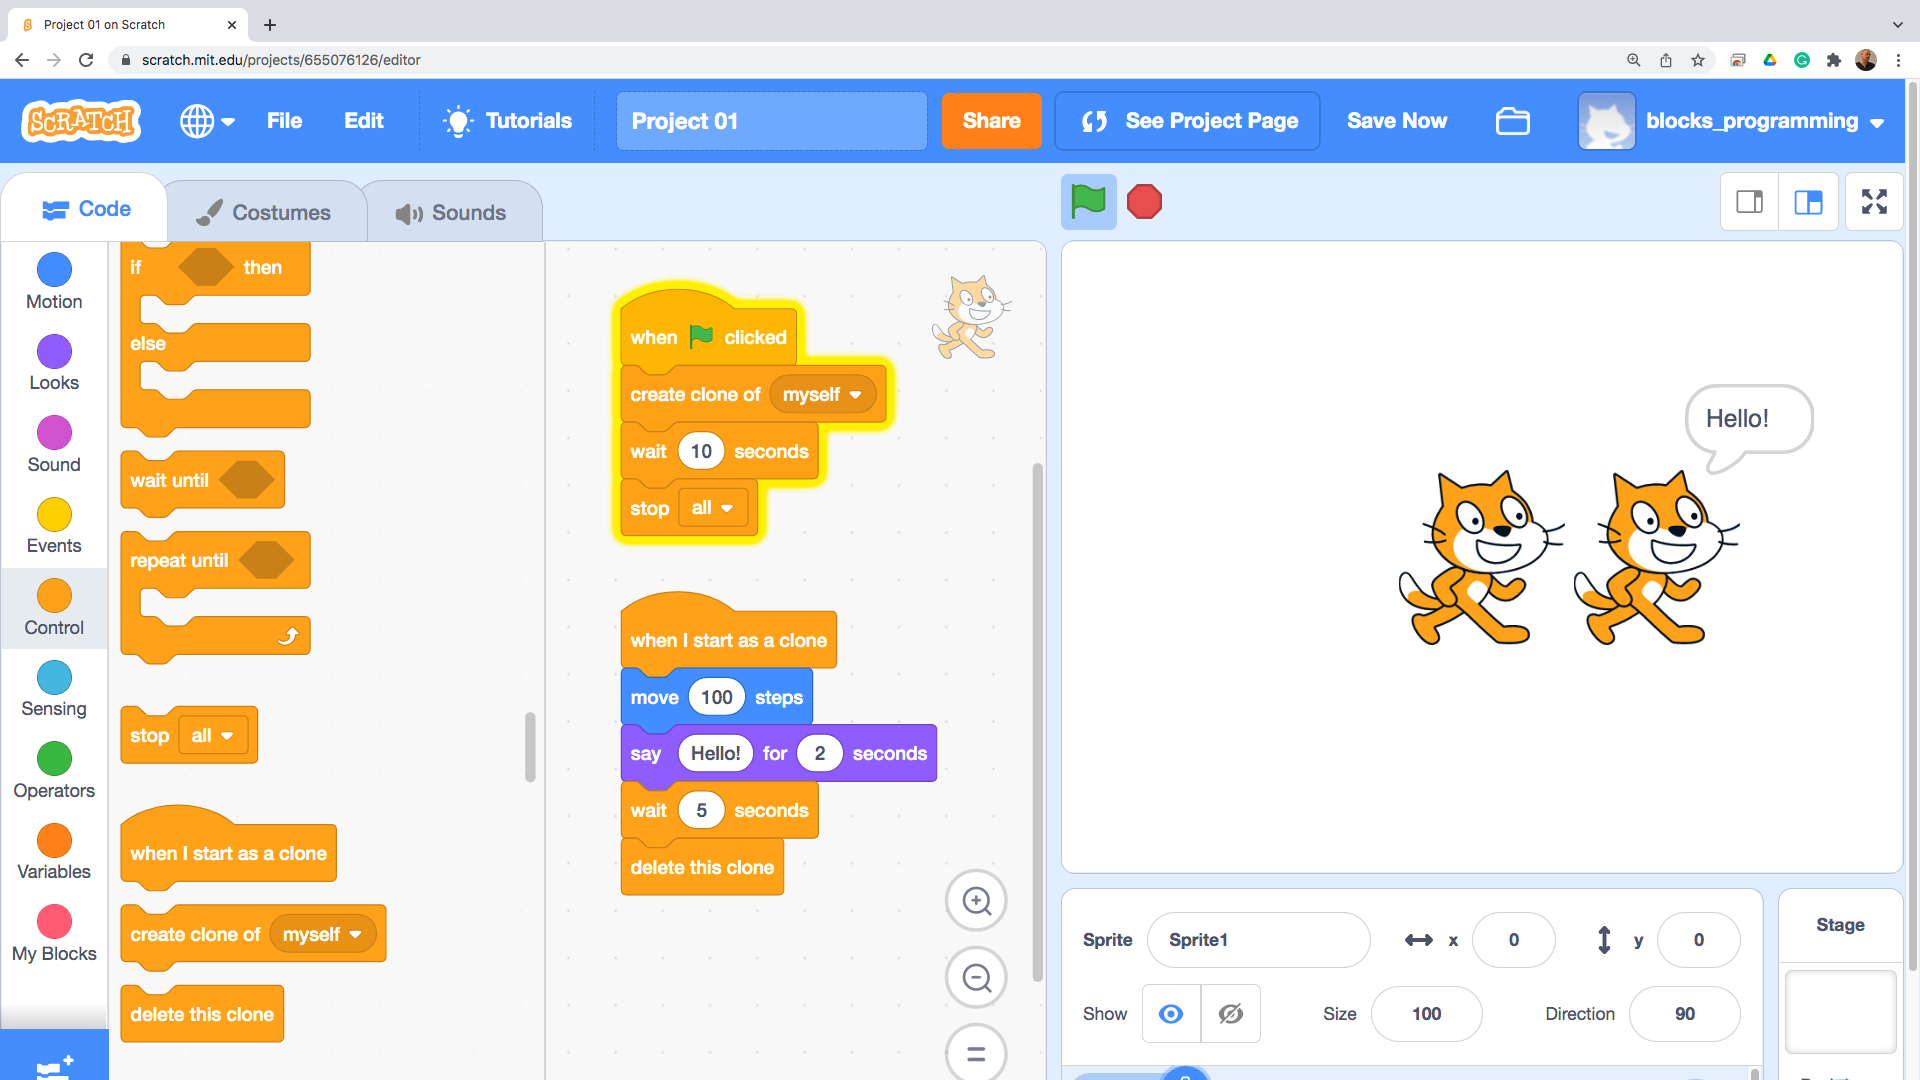
\includegraphics[width=1.0\linewidth,height=0.5\linewidth]{fig020040.png}
  \caption{Клониране на спрайтове}
\label{fig020040}
\end{figure}

Групата на светлосините блокчета е посветена на взаимодействия, отнасящите се до спрайта. Второто блокче в групата е предвидено за изпълняване на условие, когато спрайтът докосне конкретен цвят. Блокчето е с шестоъгълна форма, което подсказва, че е предназначено за вграждане. За да се демонстрира работата на това блокче, ще се завърти един цикъл, който ще премества котето на случайни координати и ще изчаква малък интервал от време, преди следващото преместване (Фиг. \ref{fig020041}). 

\begin{figure}[H]
  \centering
  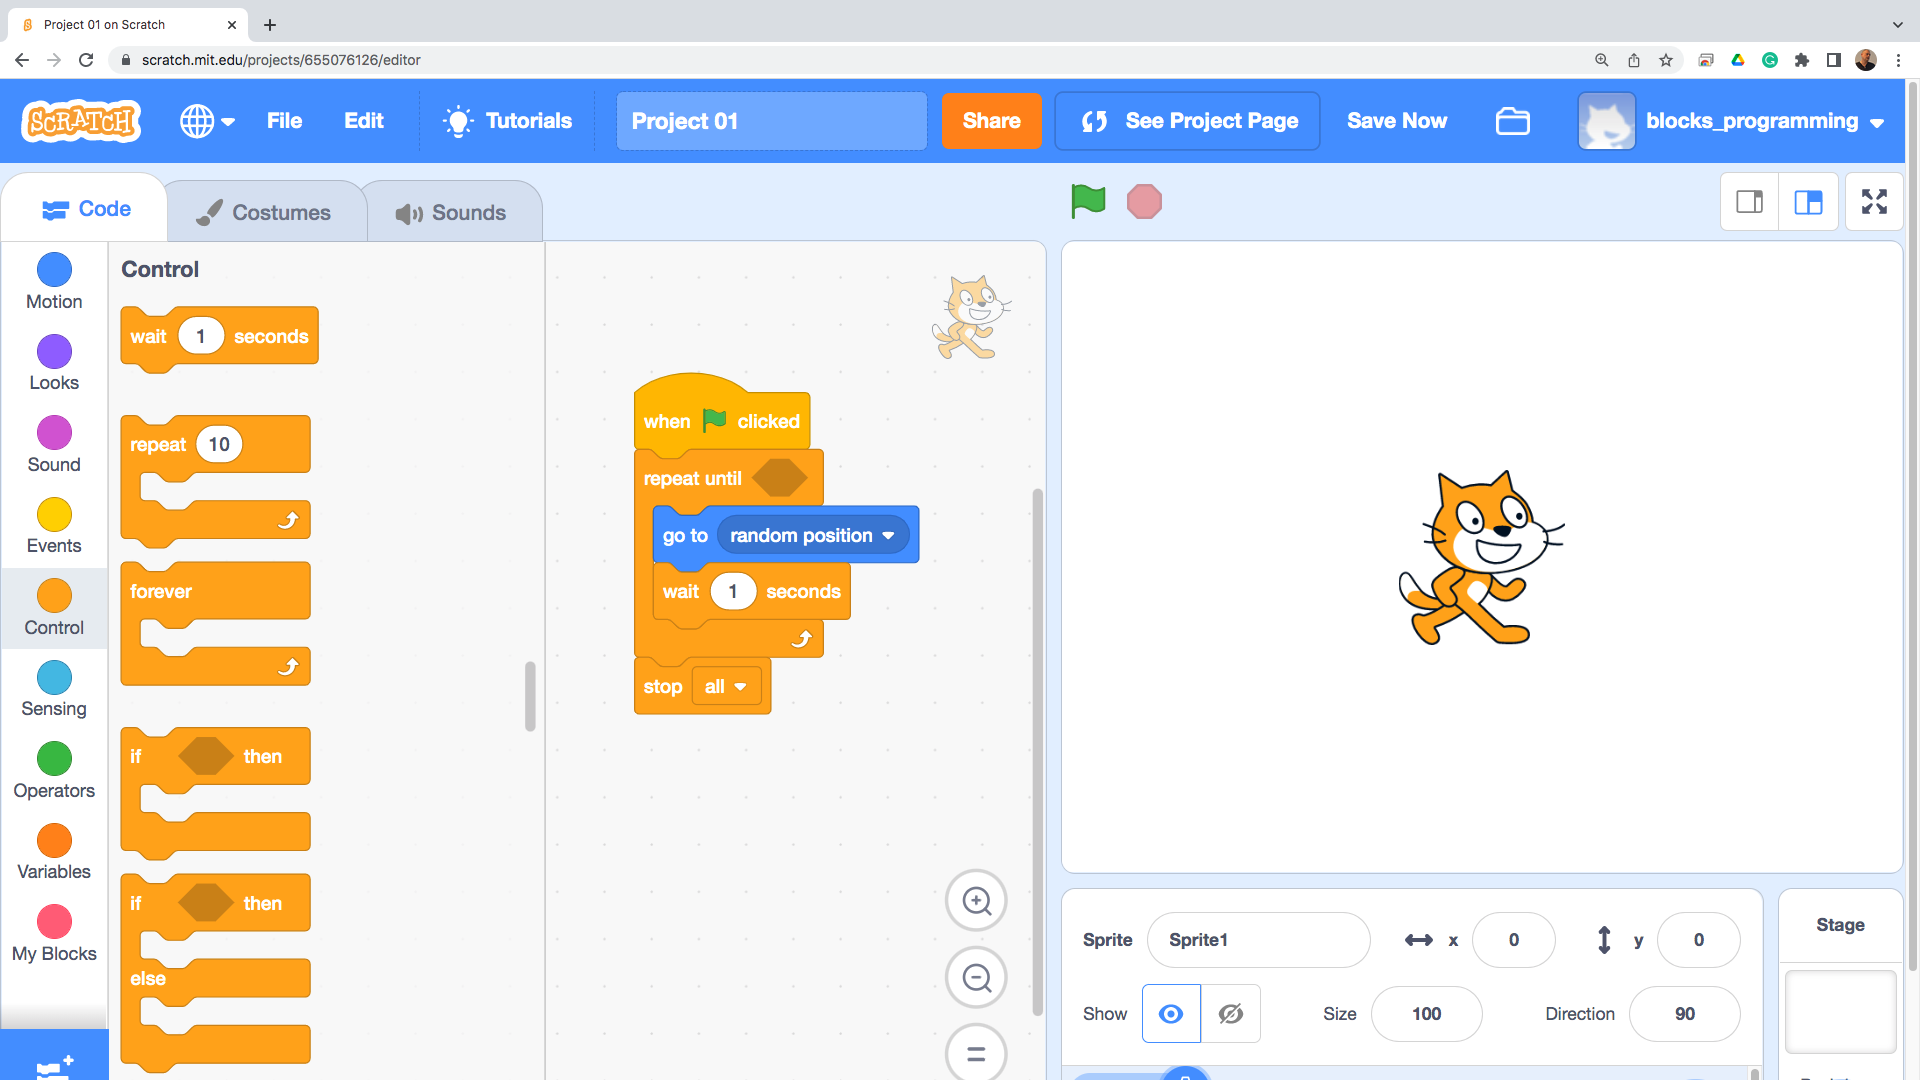
\includegraphics[width=1.0\linewidth,height=0.5\linewidth]{fig020041.png}
  \caption{Циклично прескачане на случайни координати}
\label{fig020041}
\end{figure}

Така направен цикълът ще се върти безкрайно, тъй като не е зададено условие за край. Точно в условието за край мое да се помести блокчето, определящо докосването на цвят. Към сцената ще добавим нов спрайт (Фиг. \ref{fig020042}), на една червена ябълка (Фиг. \ref{fig020043}), която котето трябва да хване. Щом я хване, ще спре да подсказа и ще измяука (Фиг. \ref{fig020044}). 

\begin{figure}[H]
  \centering
  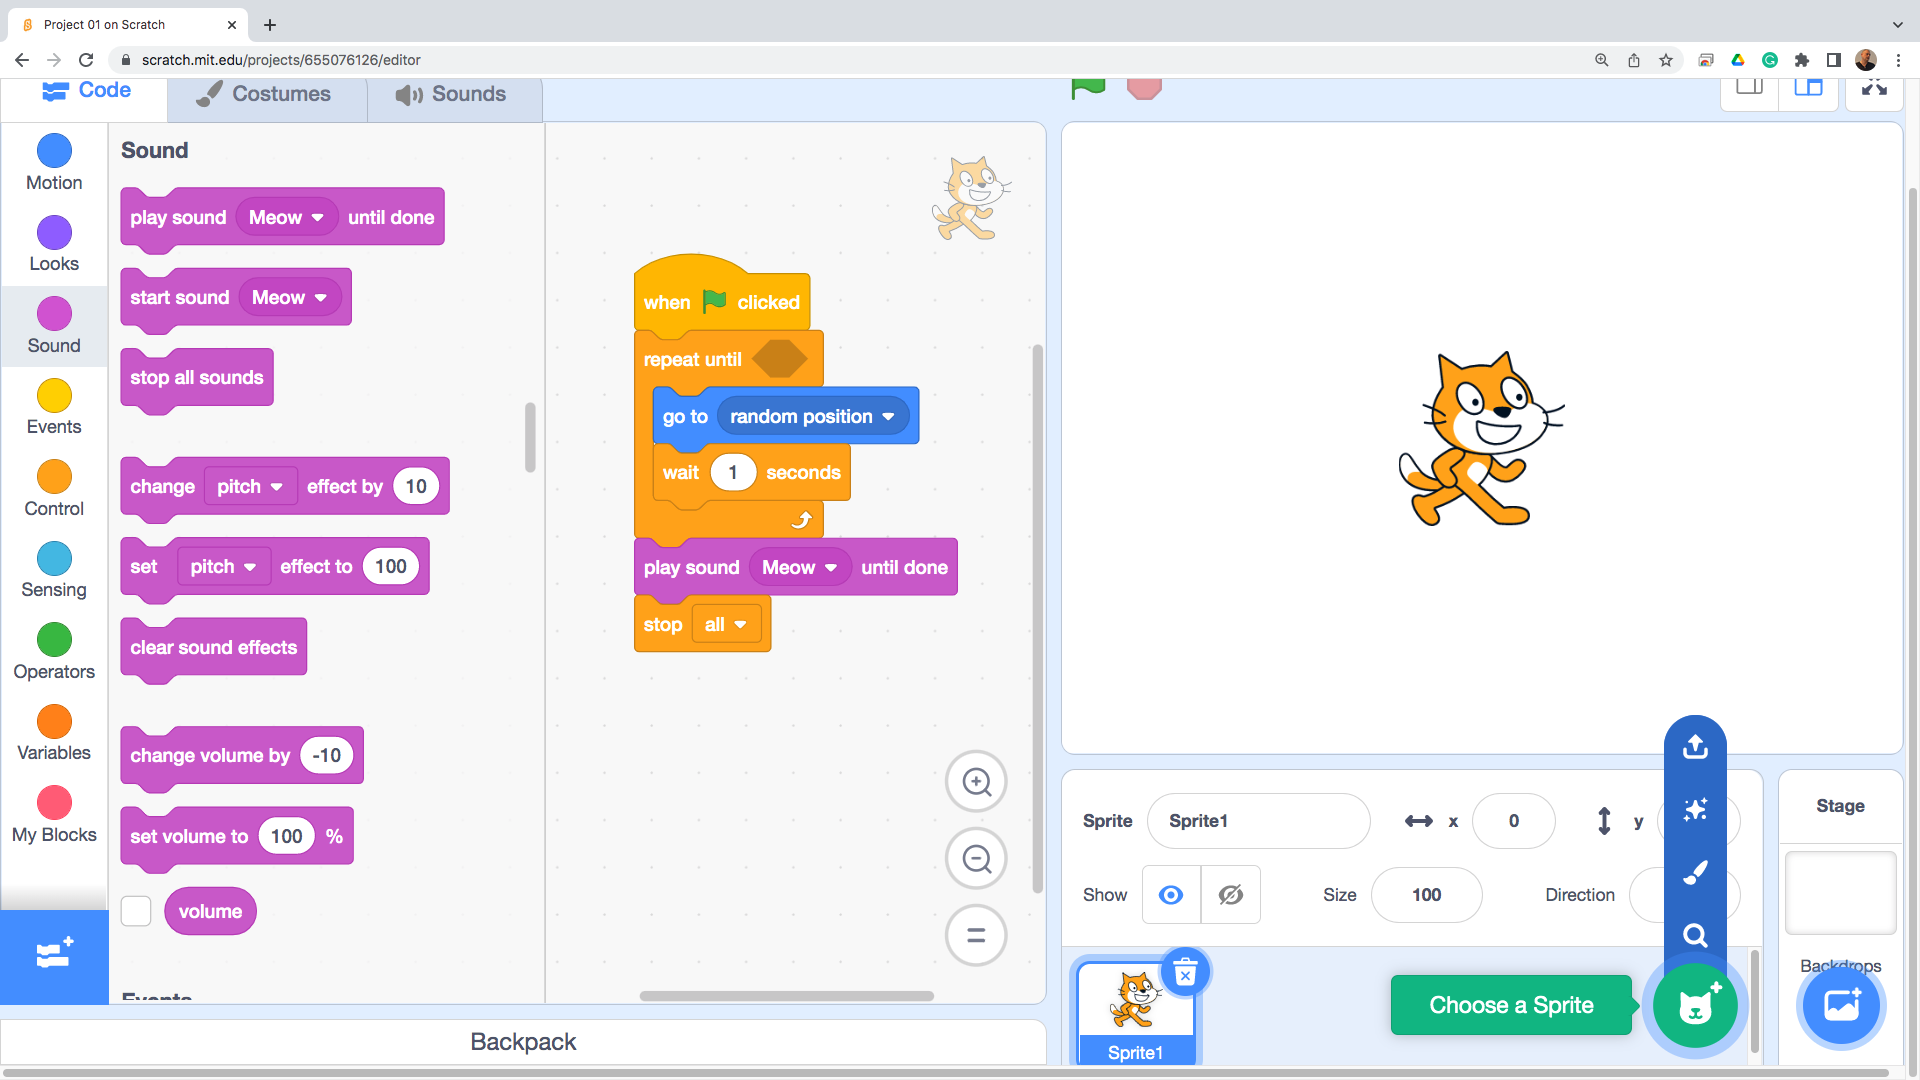
\includegraphics[width=1.0\linewidth,height=0.5\linewidth]{fig020042.png}
  \caption{Добавяне на спрайт}
\label{fig020042}
\end{figure}

\begin{figure}[H]
  \centering
  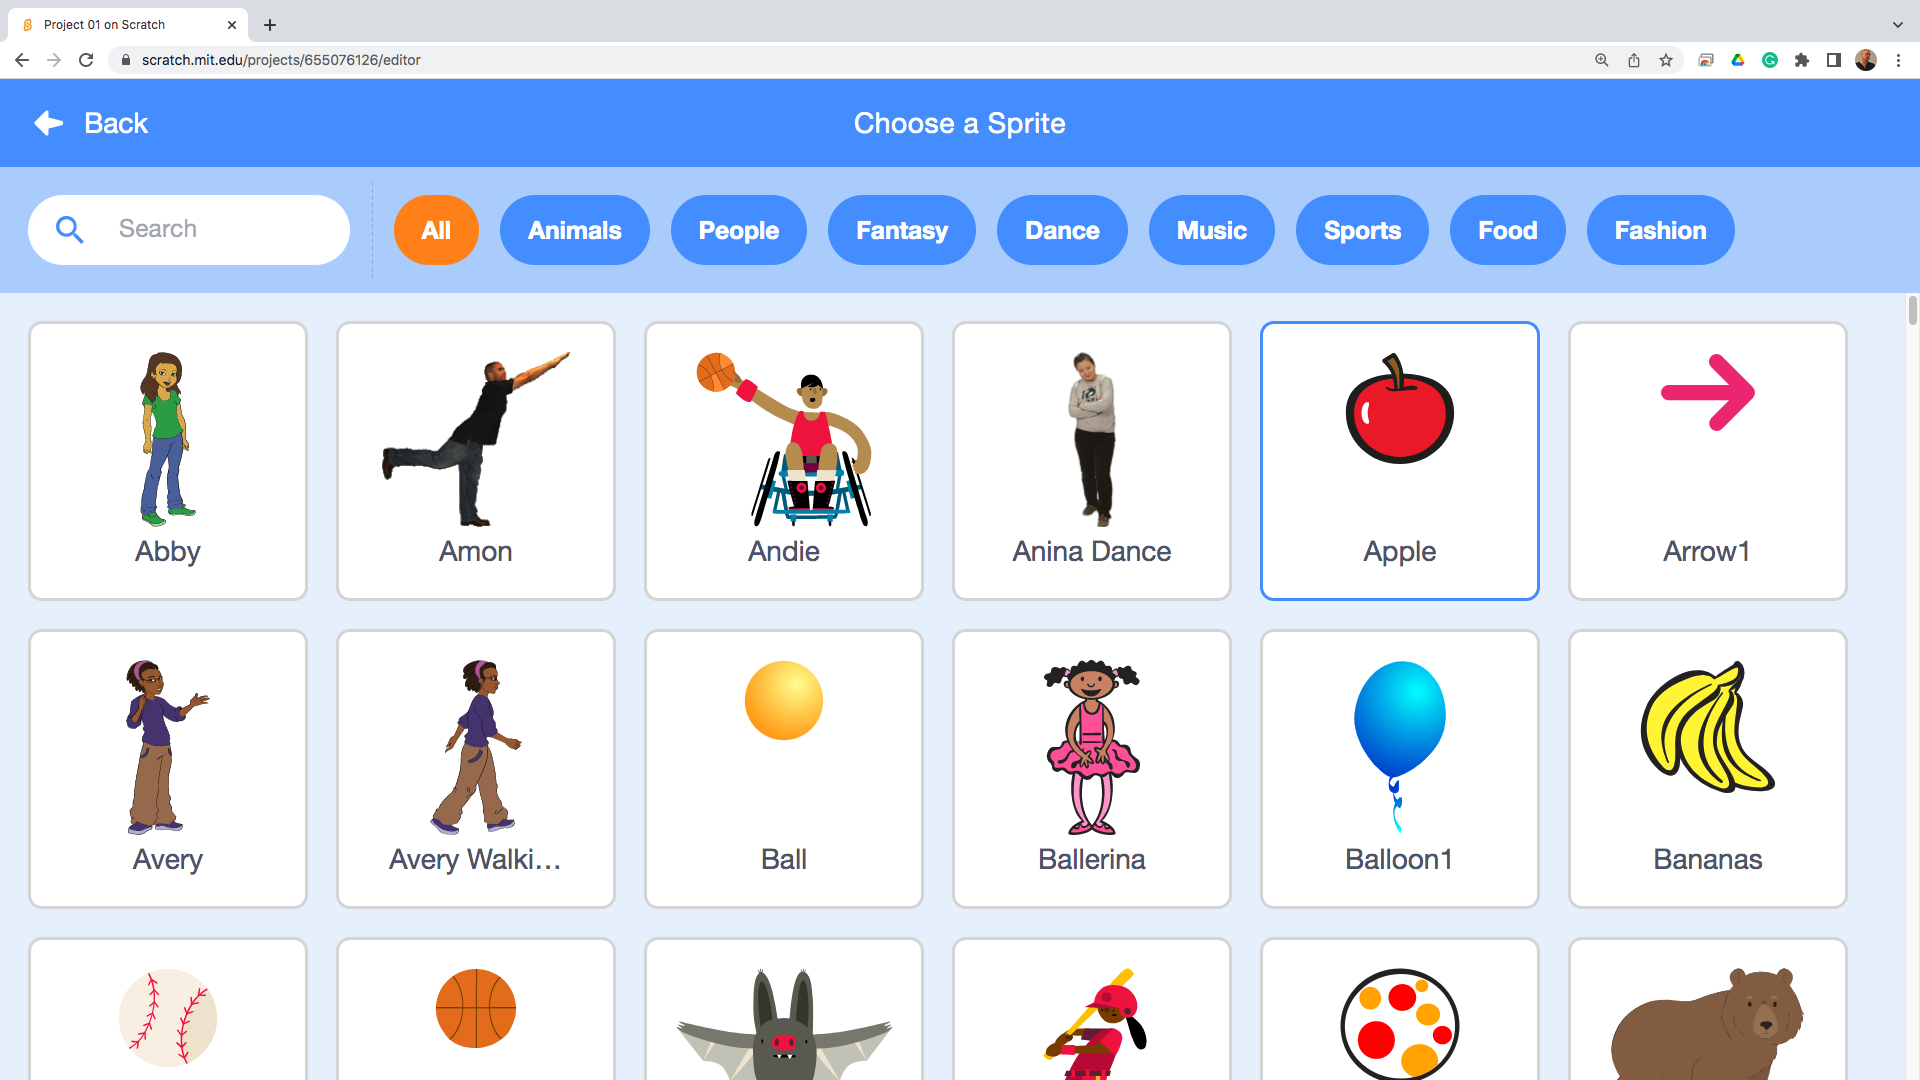
\includegraphics[width=1.0\linewidth,height=0.5\linewidth]{fig020043.png}
  \caption{Избор на спрайт от галерията}
\label{fig020043}
\end{figure}

\begin{figure}[H]
  \centering
  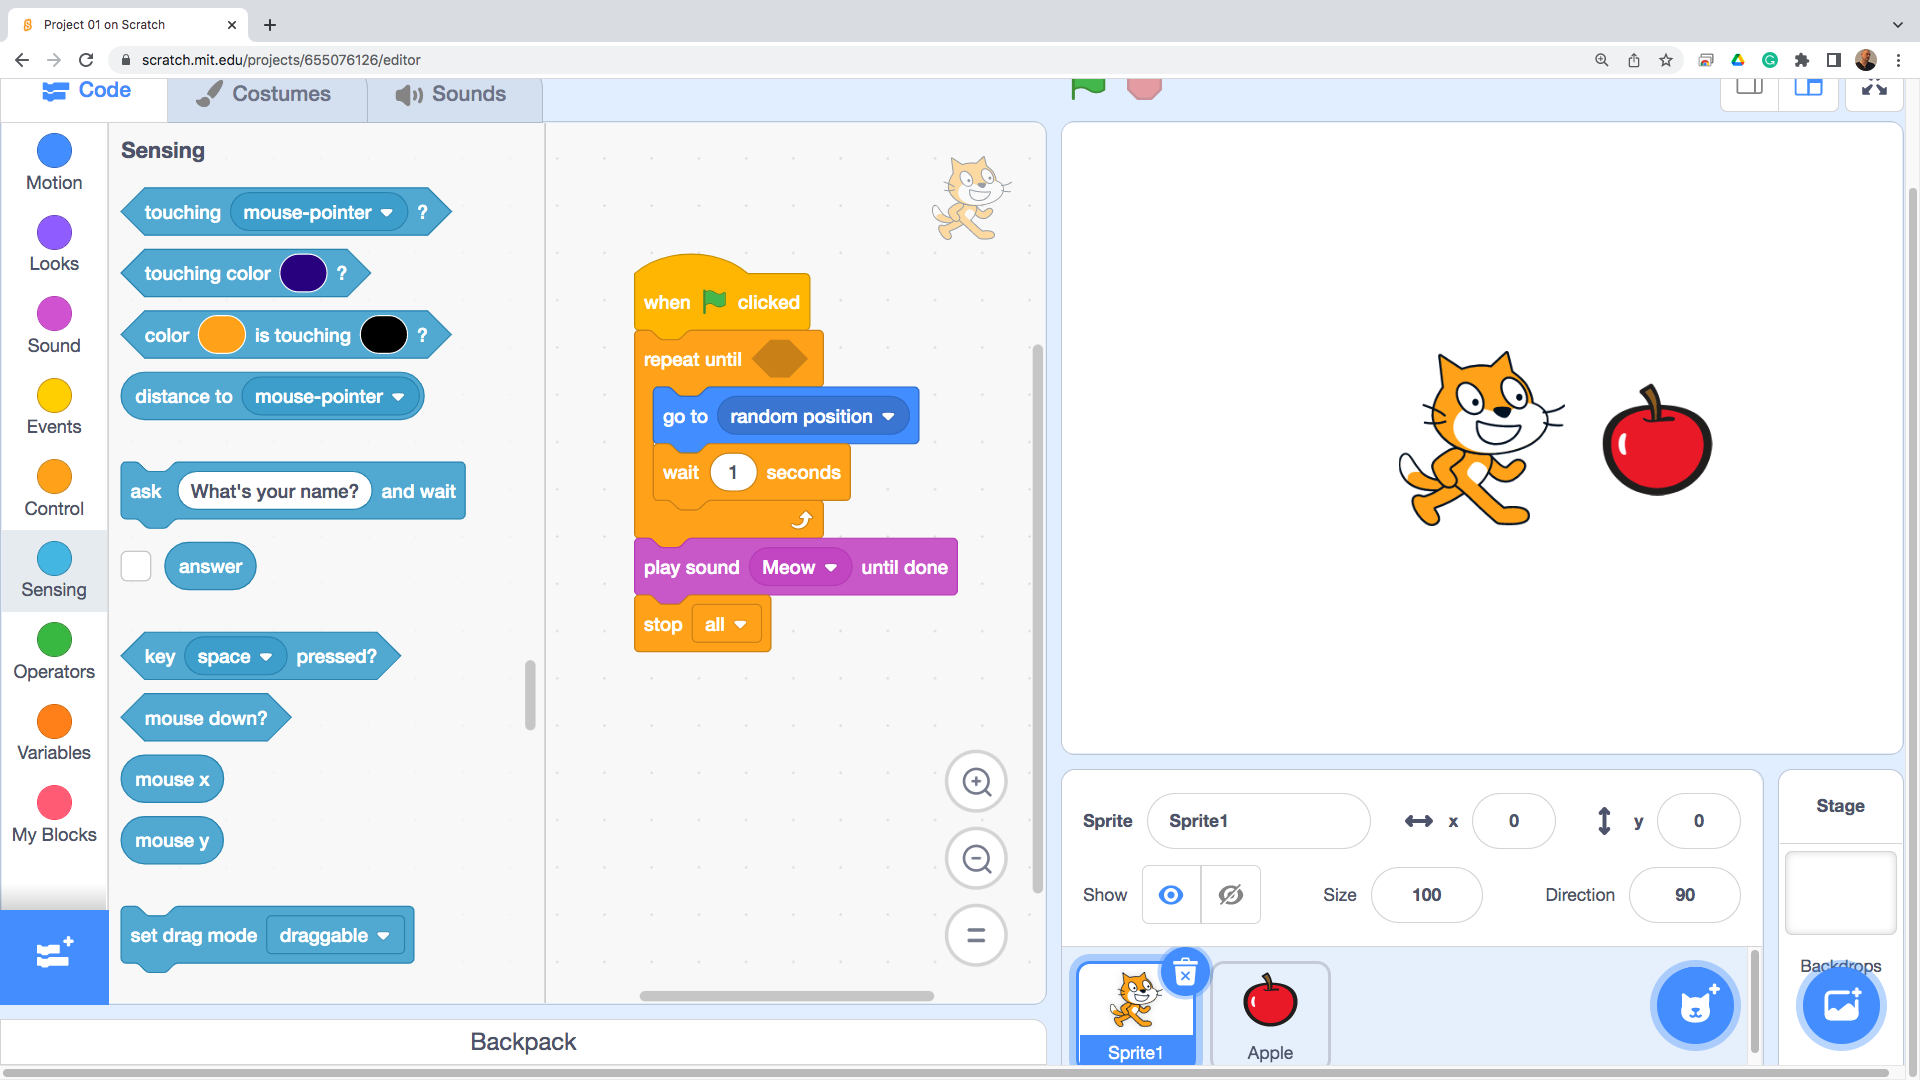
\includegraphics[width=1.0\linewidth,height=0.5\linewidth]{fig020044.png}
  \caption{Позициониране на ябълката}
\label{fig020044}
\end{figure}

При работата със спрайтове, една от най-често решаваните задачи е дали два спрайта се докосват или припокриват. Има различни техники за установяване на колизии между спрайтове, но една от най-ефективните е докосването на определен цвят. При съвременните компютри се работи с малко над 16 милиона различни цвята. Едно разумно подбиране на цветовете, които имат героите, може да даде безгранични възможности за откриване на колизии. Тъй като ябълката е червена, изборът за край на цикъла е когато котето докосне червения цвят (Фиг. \ref{fig020045}).

\begin{figure}[H]
  \centering
  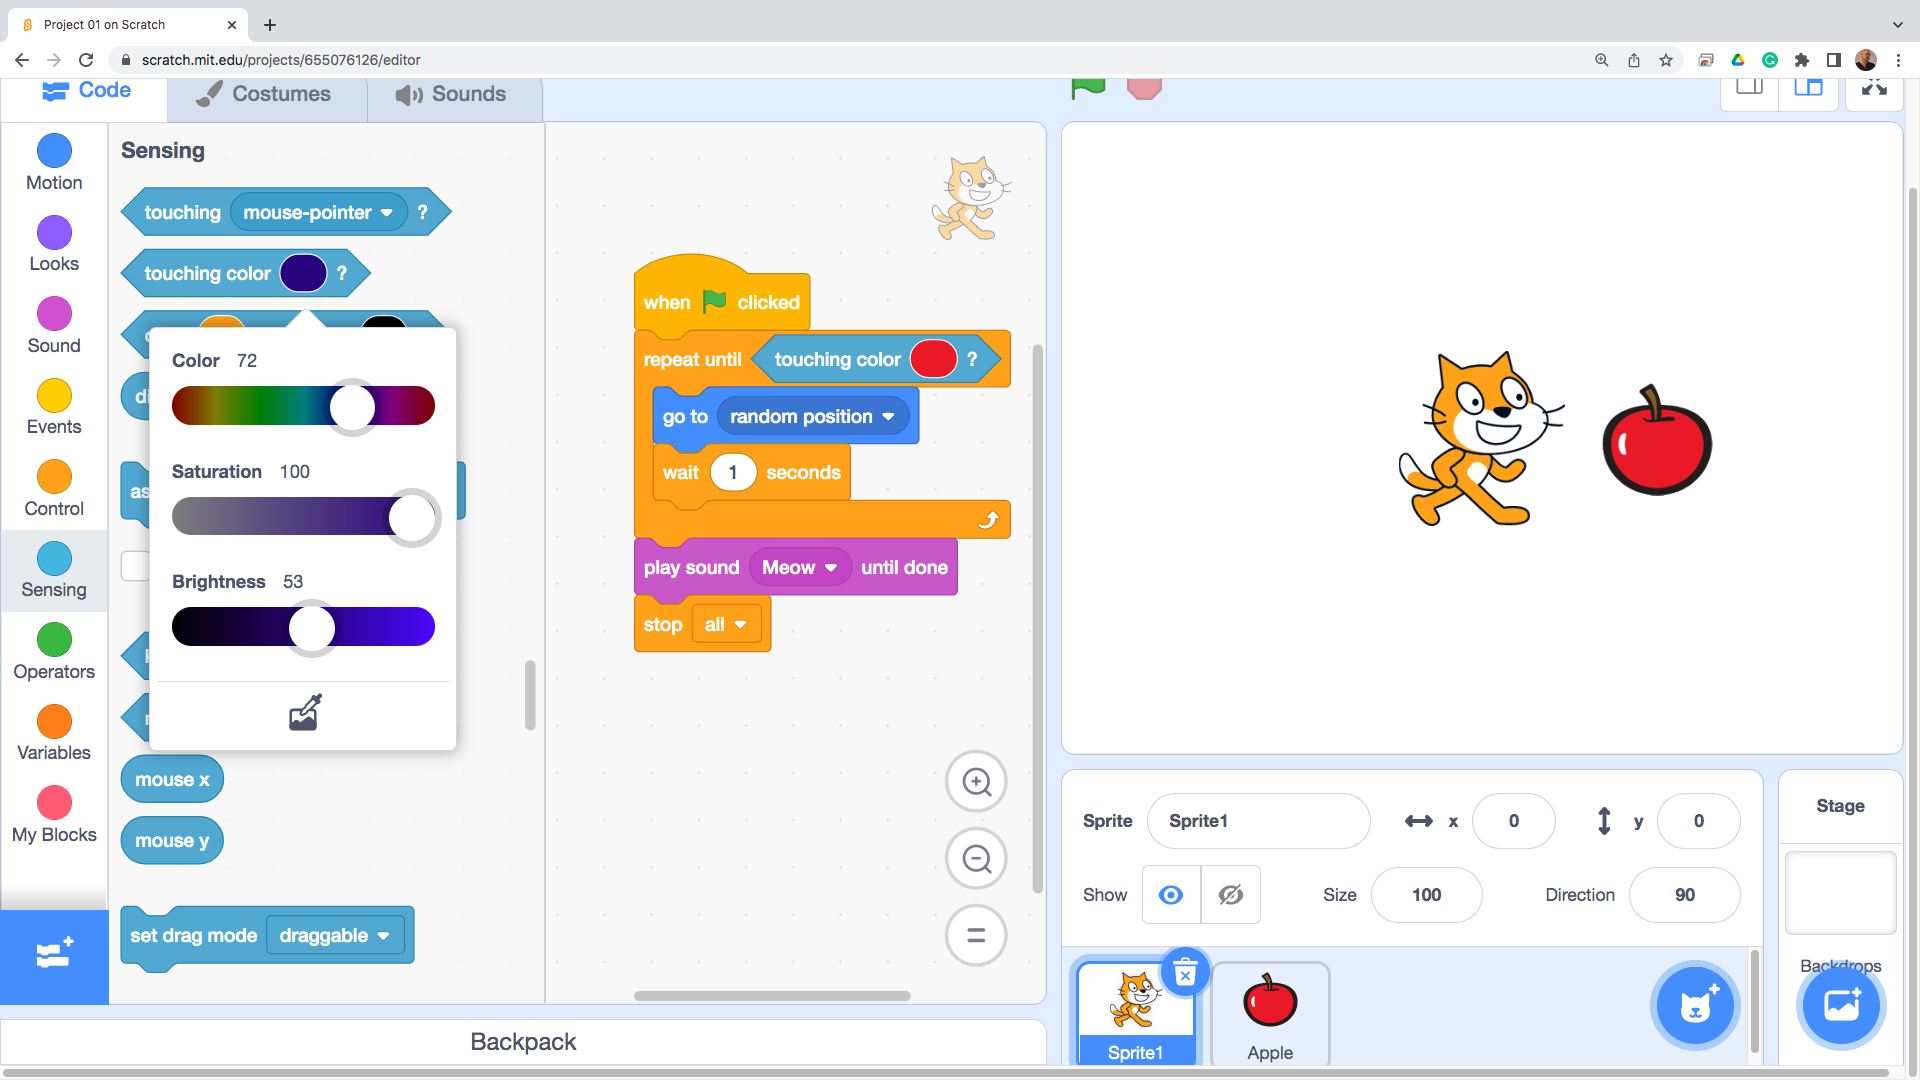
\includegraphics[width=1.0\linewidth,height=0.5\linewidth]{fig020045.png}
  \caption{Докосване по цвят}
\label{fig020045}
\end{figure}

С предходното блокче, независимо коя част на котето докосне ябълката, цикълът спира да се върти и се чува мяукането. Много по-фино определяне на колизията между спрайтовете може да се получи, ако само черният контур на котето се проверява за докосване до червения цвят на ябълката, за което служи следващото блокче (Фиг. \ref{fig020046}).

\begin{figure}[H]
  \centering
  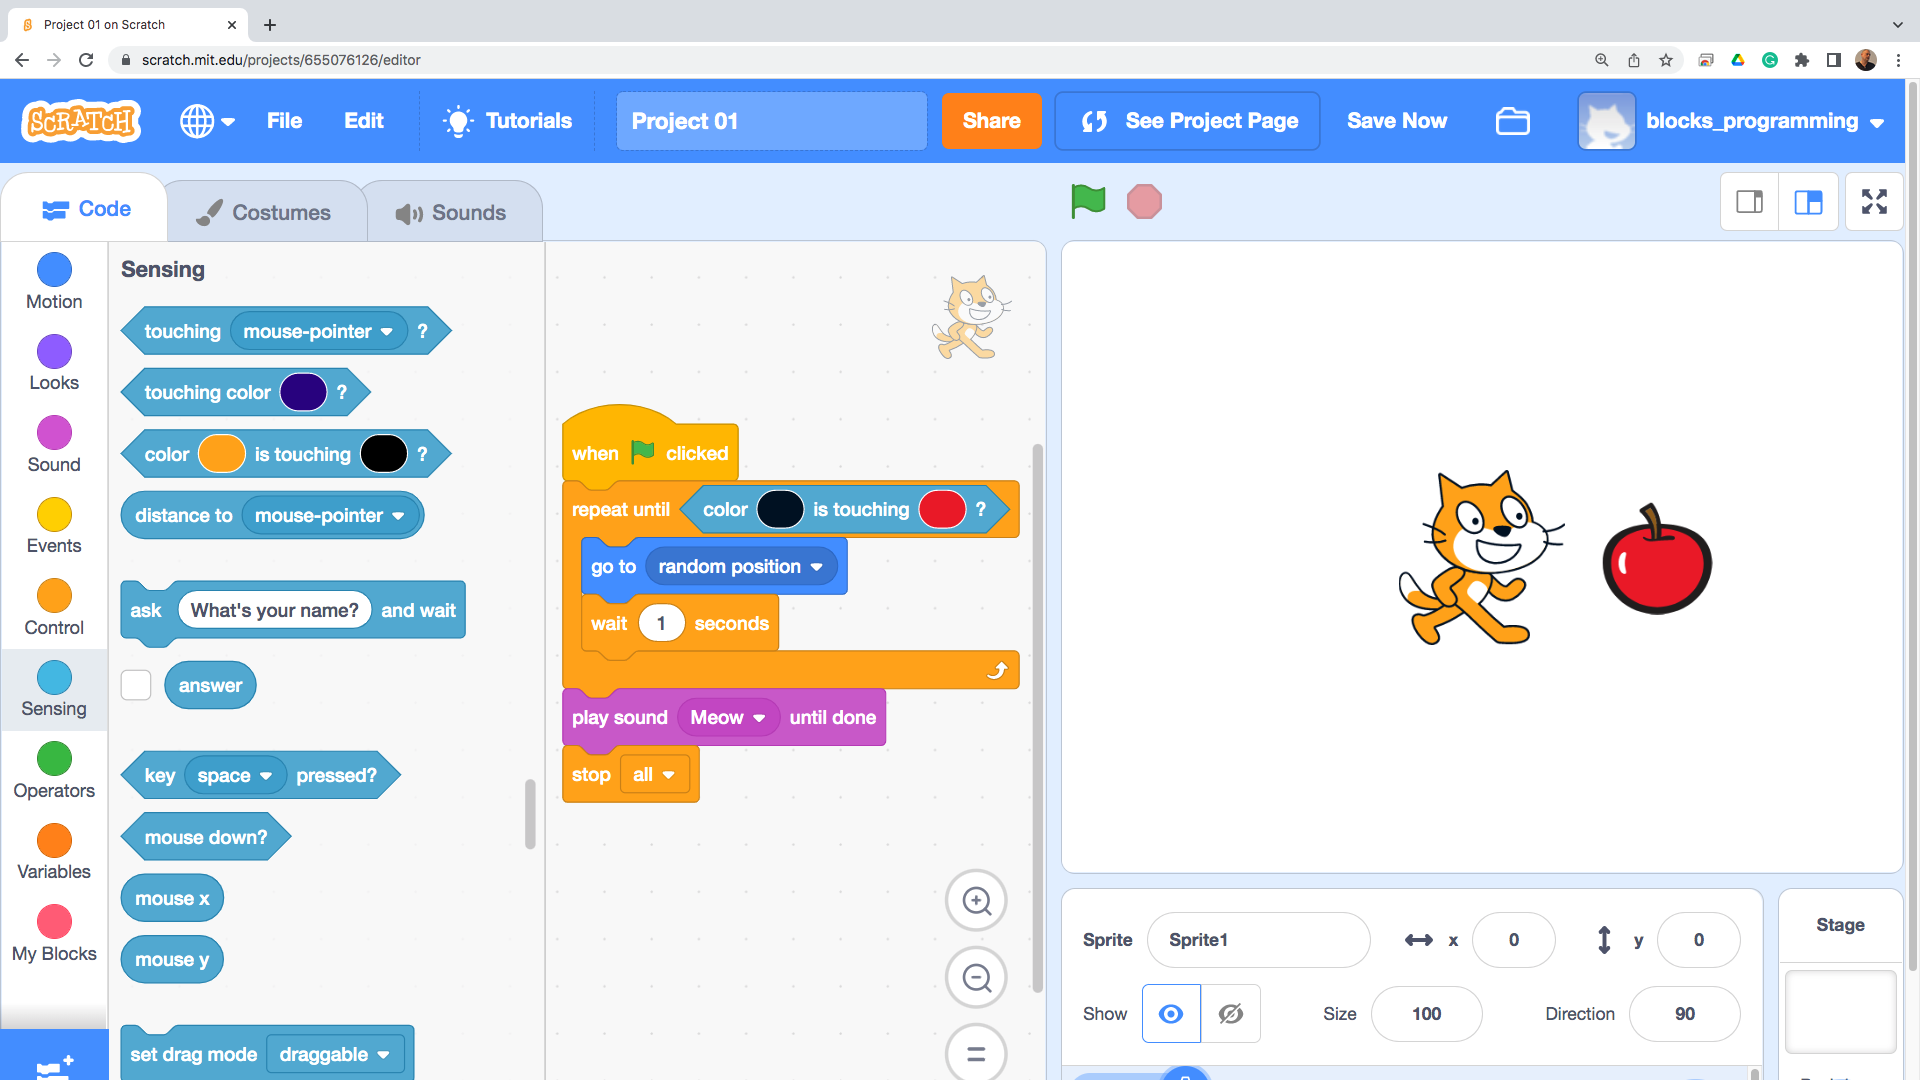
\includegraphics[width=1.0\linewidth,height=0.5\linewidth]{fig020046.png}
  \caption{Колизия при два предварително зададени цвята}
\label{fig020046}
\end{figure}

Следващото блокче е с овална форма и доставя на програмата разстоянието между спрайта и показалеца на мишката. Овалната форма подсказва, че това блокче трябва да бъде вградено в някое от блокчетата за аритметични изрази (Фиг. \ref{fig020047}).

\begin{figure}[H]
  \centering
  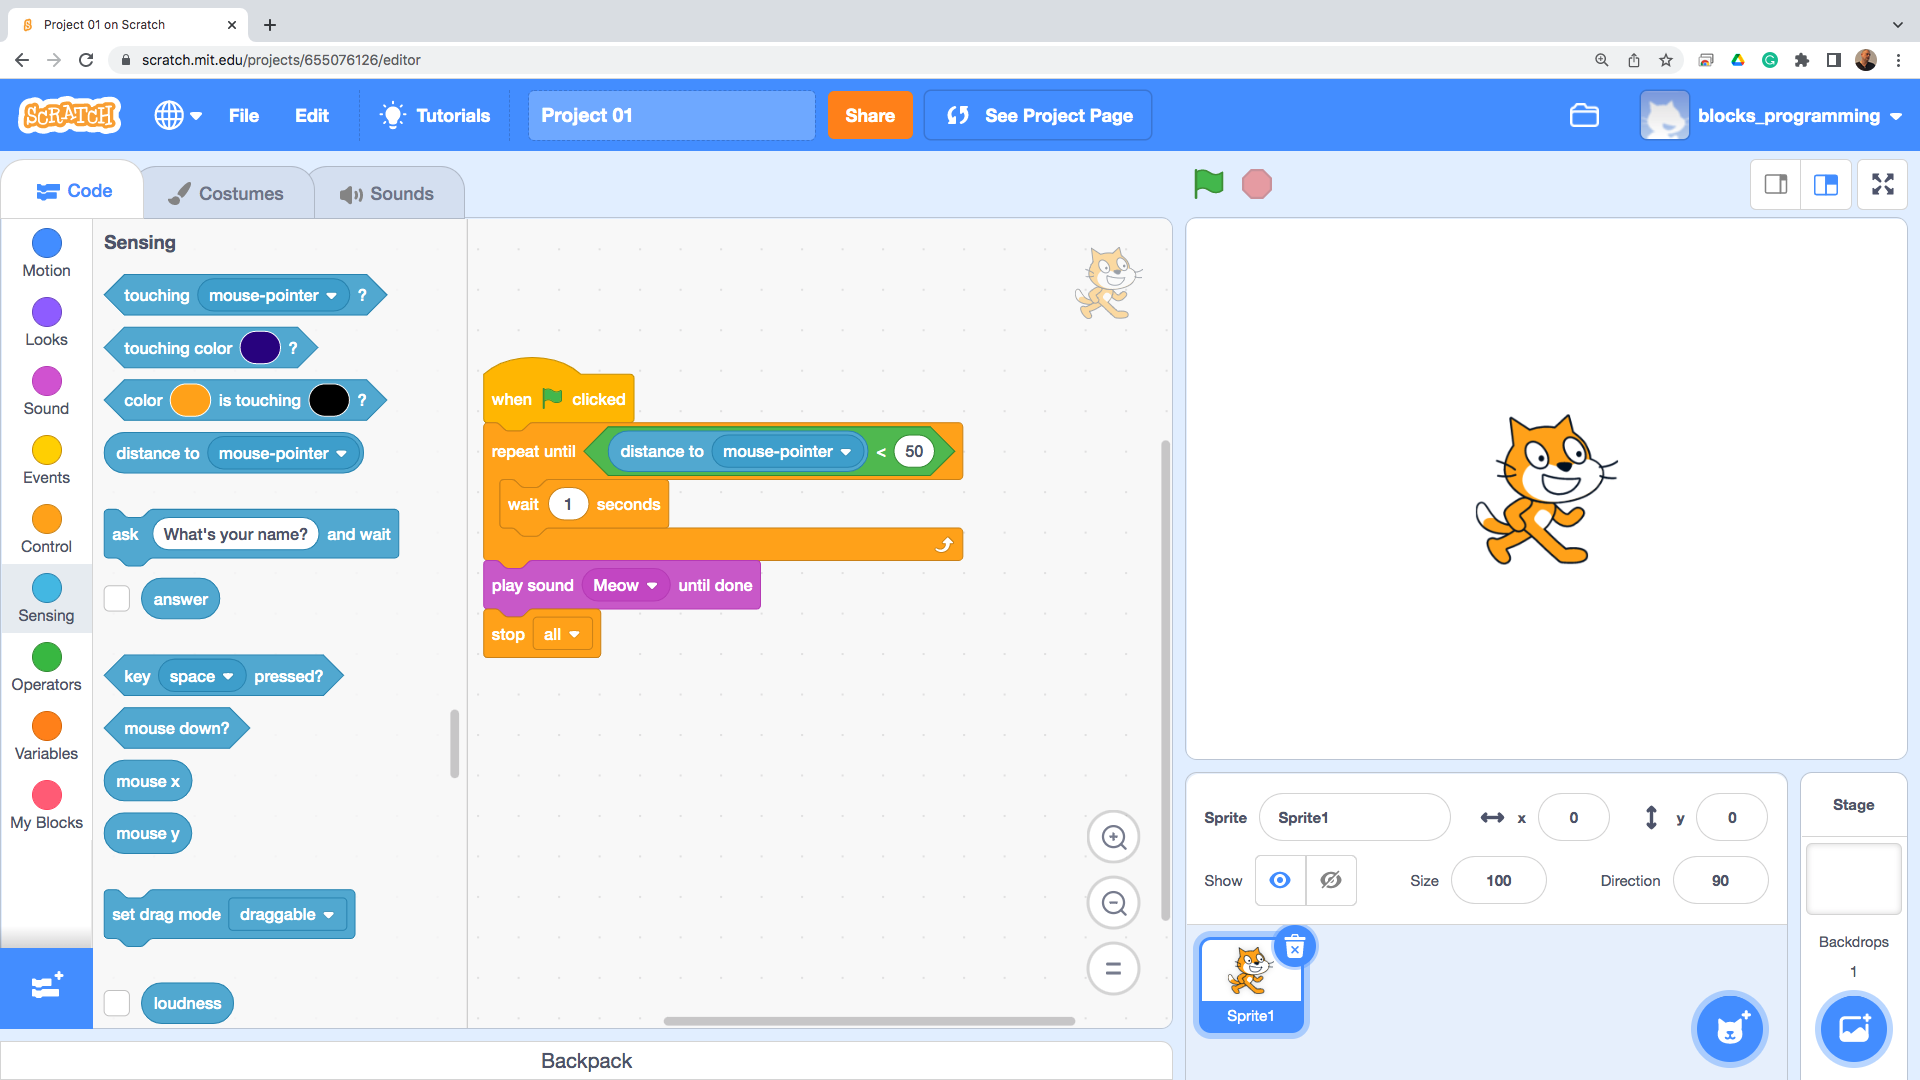
\includegraphics[width=1.0\linewidth,height=0.5\linewidth]{fig020047.png}
  \caption{Разстояние до показалеца на мишката}
\label{fig020047}
\end{figure}

Понякога се налага потребителят да напише нещо. За да се даде тази възможност е следващото блокче в групата на светло сините (Фиг. \ref{fig020048}). Анимираният герой подканя потребителя, като в конкретен текст подсказва какво се очаква да бъде написано. 

\begin{figure}[H]
  \centering
  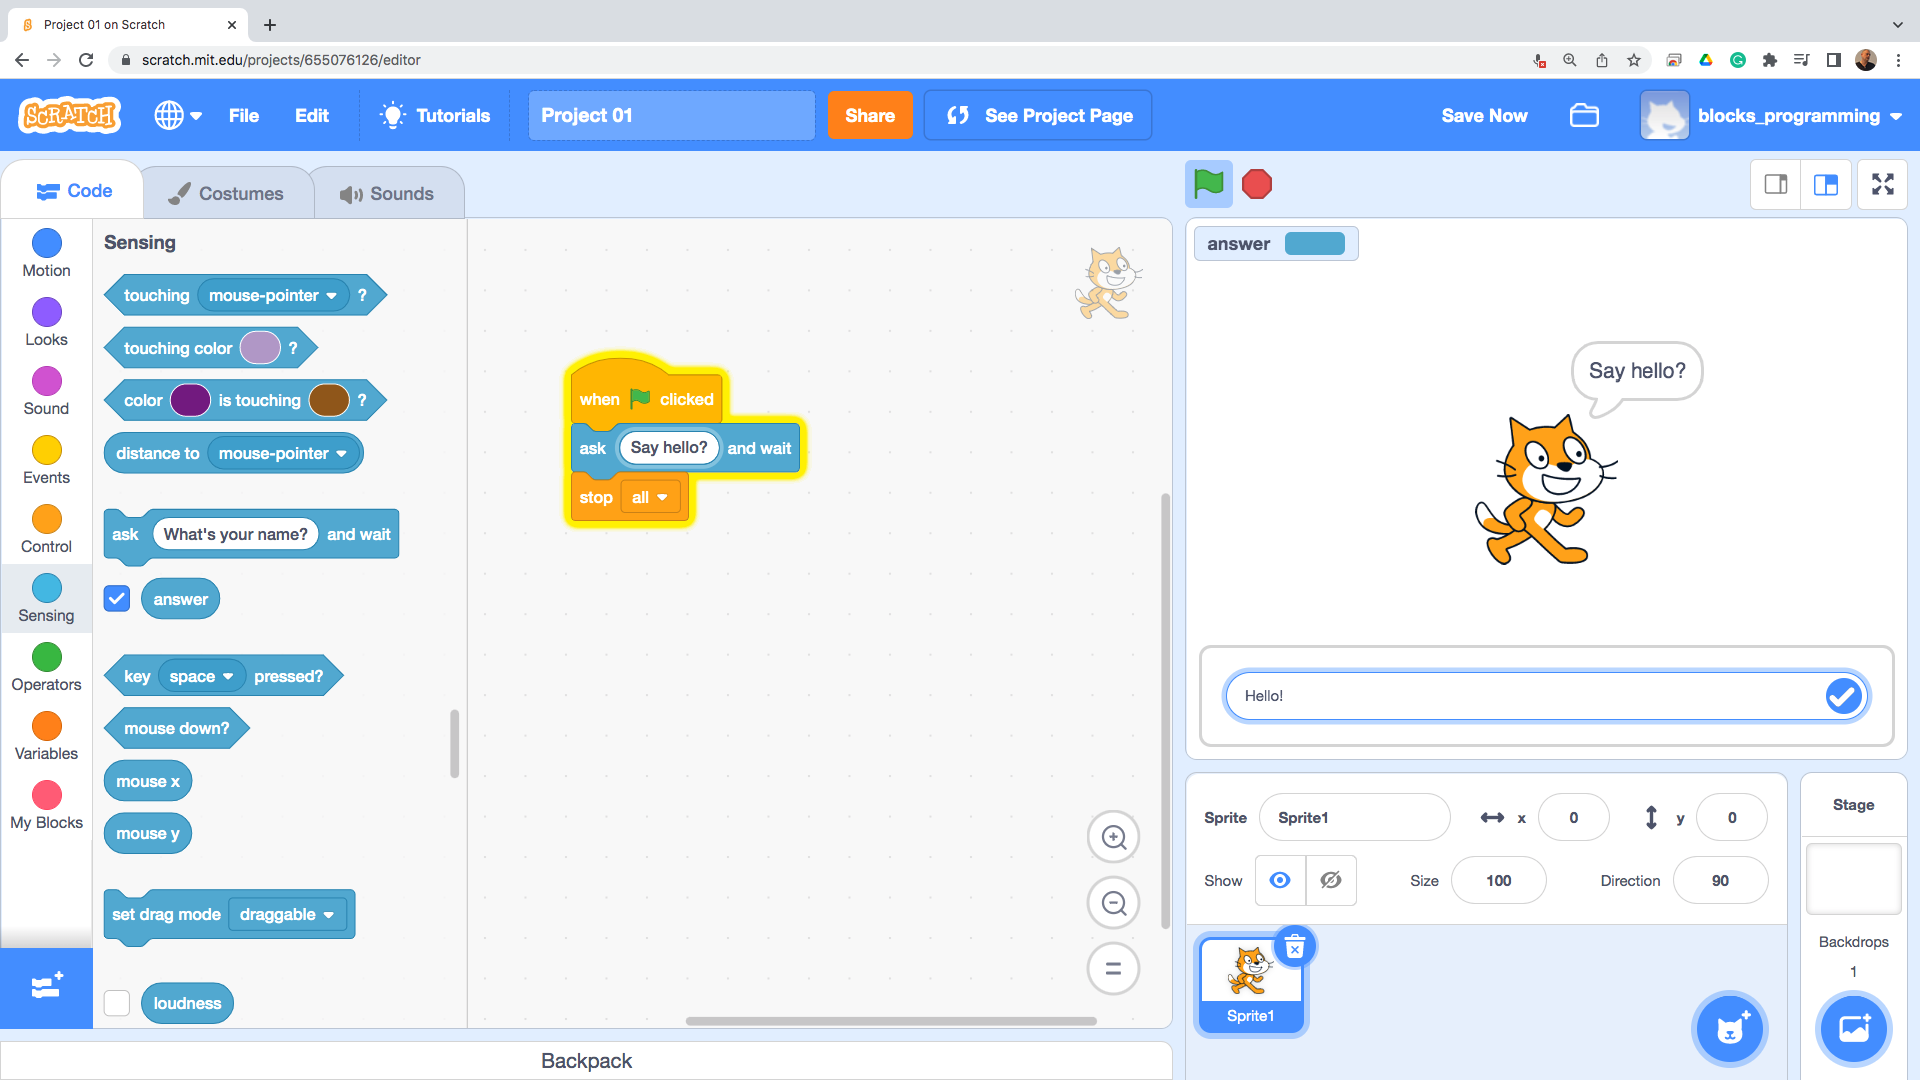
\includegraphics[width=1.0\linewidth,height=0.5\linewidth]{fig020048.png}
  \caption{Въвеждане на текст}
\label{fig020048}
\end{figure}

Следващото блокче е от шестоъгълните и е предназначено за вграждане. Това блокче връща резултат „истина“, когато бъде натиснат определен клавиш (Фиг. \ref{fig020049}).

\begin{figure}[H]
  \centering
  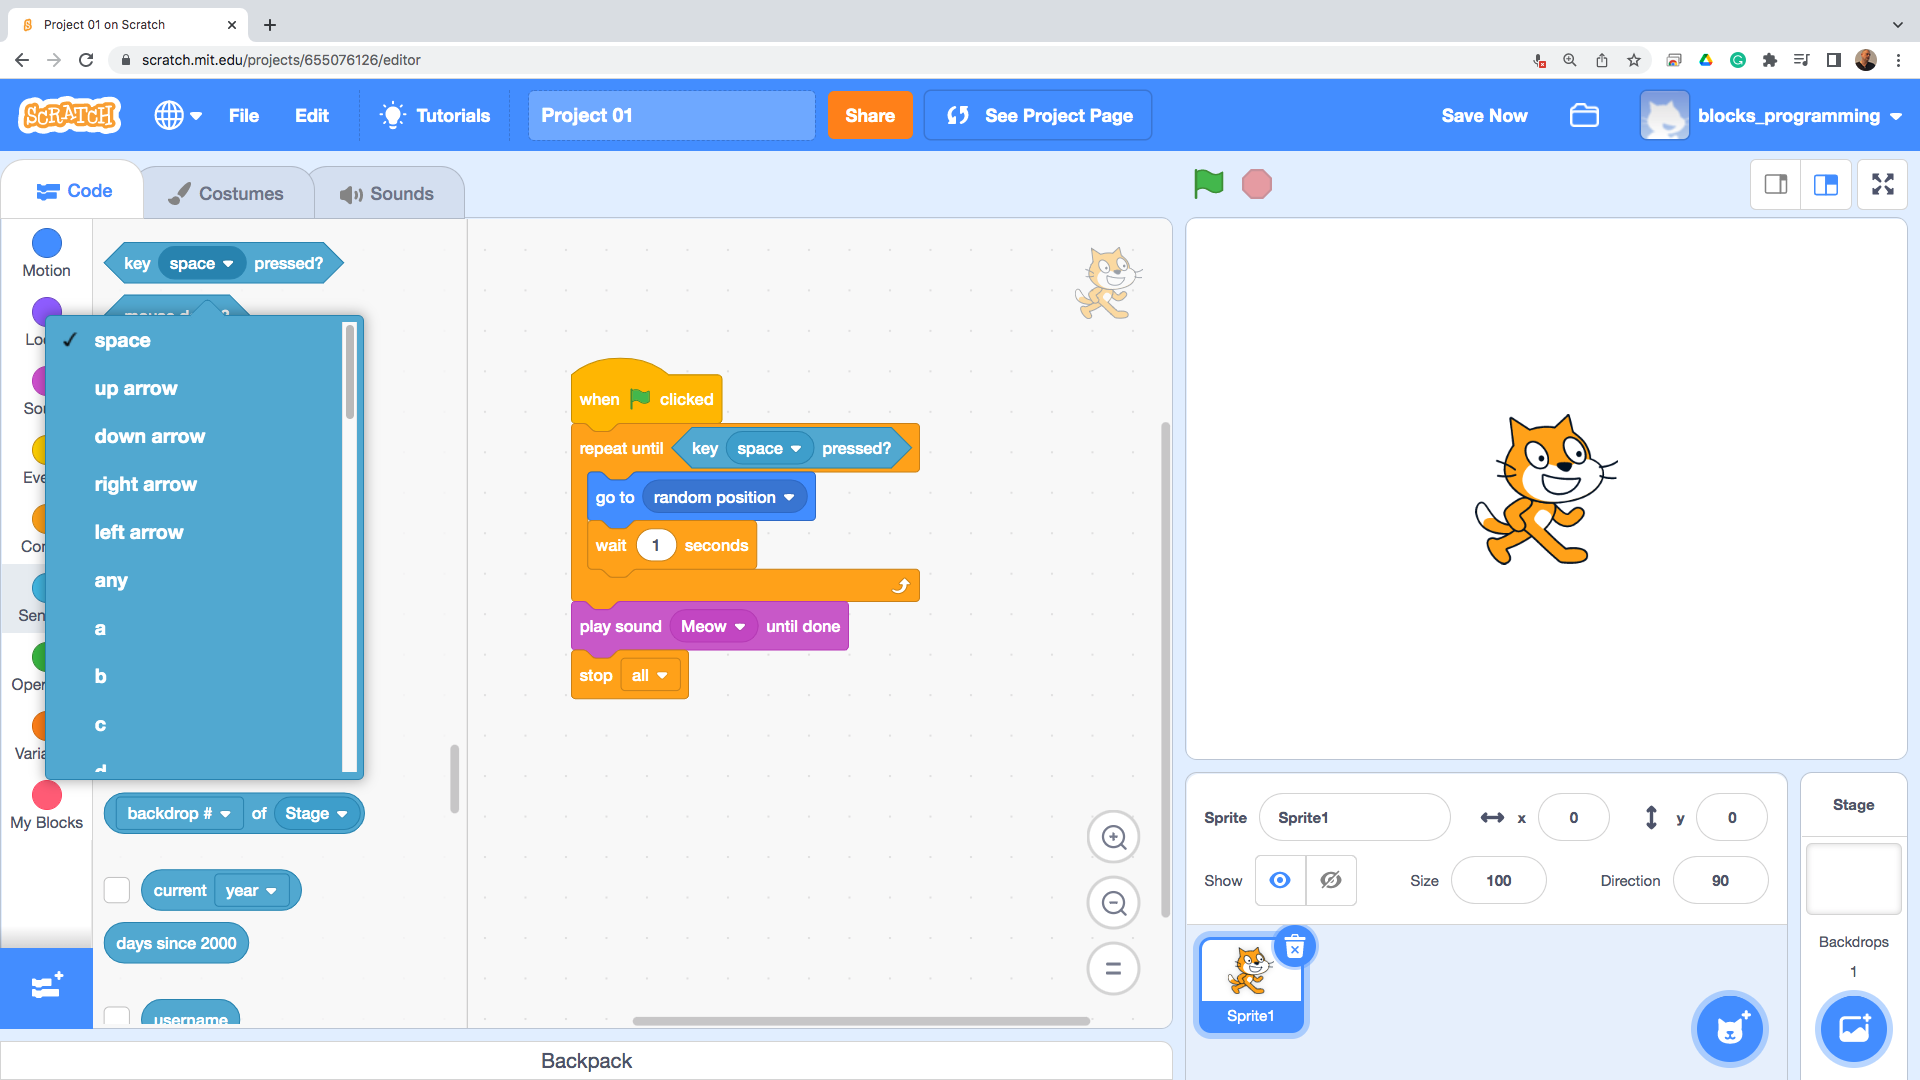
\includegraphics[width=1.0\linewidth,height=0.5\linewidth]{fig020049.png}
  \caption{Определяне на натиснат клавиш}
\label{fig020049}
\end{figure}

Сходно поведение може да се постигне и със следващото блокче, но вместо натискане на клавиш от клавиатурата се очаква натискане на клавиша на мишката (Фиг. \ref{fig020050}).

\begin{figure}[H]
  \centering
  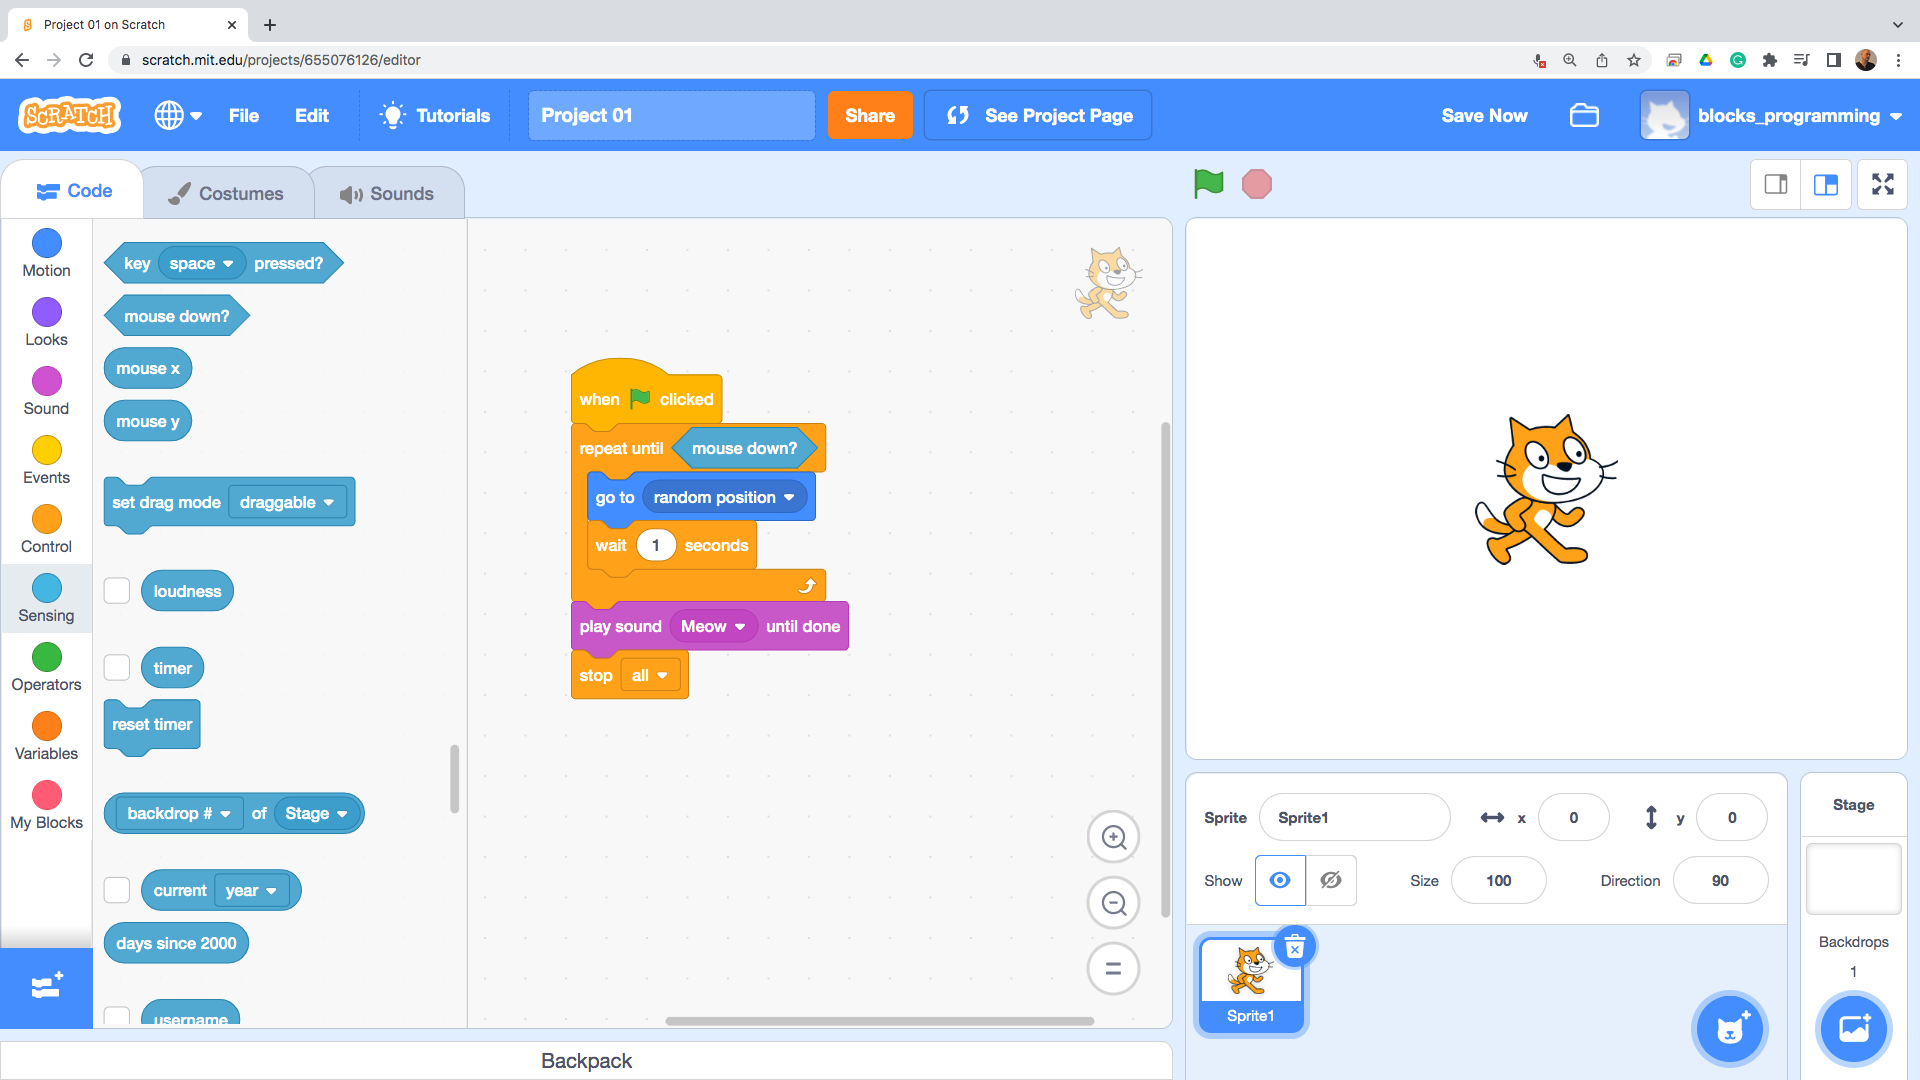
\includegraphics[width=1.0\linewidth,height=0.5\linewidth]{fig020050.png}
  \caption{Определяне на натиснат бутон от мишката}
\label{fig020050}
\end{figure}

Следващите две блокчета са овални и също са за вграждане. Първото дава координатите на анимирания герой по абцисната ос, а второто дава координатите на анимирания герой по ординатната ос (Фиг. \ref{fig020051}).

\begin{figure}[H]
  \centering
  \includegraphics[width=1.0\linewidth,height=0.5\linewidth]{fig020051.png}
  \caption{Координати на анимирания герой}
\label{fig020051}
\end{figure}

По време на работа на програмата има функциониращ таймер, който отмерва времето от началото на изпълнението. Със следващото блокче този таймер може да се нулира (Фиг. \ref{fig020052}).

\begin{figure}[H]
  \centering
  \includegraphics[width=1.0\linewidth,height=0.5\linewidth]{fig020052.png}
  \caption{Нулиране на таймера}
\label{fig020052}
\end{figure}

Следващото блокче е от овалните и служи за доставяне на информация за фона, променливи или нивото на звука (Фиг. \ref{fig020053}).

\begin{figure}[H]
  \centering
  \includegraphics[width=1.0\linewidth,height=0.5\linewidth]{fig020053.png}
  \caption{Информация за компоненти от сцената}
\label{fig020053}
\end{figure}

Последното блокче в групата е предвидено също за вграждане и връща броя дни от година 2000 (Фиг. \ref{fig020054}).

\begin{figure}[H]
  \centering
  \includegraphics[width=1.0\linewidth,height=0.5\linewidth]{fig020054.png}
  \caption{Брой дни от началото на века}
\label{fig020054}
\end{figure}

Групата на зелените блокчета е предназначена за вграждане. Първите четири блокчета са с овална форма и са предвидени за аритметичните операции – събиране, изваждане, умножение и делене (Фиг. \ref{fig020055}).

\begin{figure}[H]
  \centering
  \includegraphics[width=1.0\linewidth,height=0.5\linewidth]{fig020055.png}
  \caption{Аритметични операции}
\label{fig020055}
\end{figure}

Блокчето за избор на случайно число вече е демонстрирано, но то идеално пасва в трите блокчета, които следват след него. Това са блокчета за сравнение и са предвидени за вграждане в блокчетата за управление на изпълнението (Фиг. \ref{fig020056}).

\begin{figure}[H]
  \centering
  \includegraphics[width=1.0\linewidth,height=0.5\linewidth]{fig020056.png}
  \caption{Операции за сравнение}
\label{fig020056}
\end{figure}

Следват три блокчета с шестоъгълна форма (Фиг. \ref{fig020057}), които служат за вграждане в блокчета за контрол на управлението. Трите блокчета изпълняват трите основни логически операции („и“, „или“, „не“). При първото блокче и двете условия трябва да са изпълнени за да се влезе в конструкцията за условен преход. Точно поради тази причина, логическата операция се нарича „и“. При второто блокче или едното условие, или другото условие трябва да бъде изпълнено, за да се влезе в конструкцията за условен преход. Точно поради тази причина, логическата операция се нарича „или“. При третото блокче, резултата се обръща, така че в конструкцията за условен преход се влиза при невярно условие. Поради тази причина, тази операция се нарича „отрицание“.

\begin{figure}[H]
  \centering
  \includegraphics[width=1.0\linewidth,height=0.5\linewidth]{fig020057.png}
  \caption{Логически операции}
\label{fig020057}
\end{figure}

Следващите четири блокчета са за работа със символни низове (Фиг. \ref{fig020058}). Първите три са с овална форма, а последното е с шестоъгълна форма. Първото блокче слепва два символни низа. Второто блокче определя буква на определена позиция в символния низ. Третото блокче определя дължината на символния низ. Четвъртото блокче търси определена буква в символния низ. 

\begin{figure}[H]
  \centering
  \includegraphics[width=1.0\linewidth,height=0.5\linewidth]{fig020058.png}
  \caption{Работа със символни низове}
\label{fig020058}
\end{figure}

Последните три блокчета в групата на зелените са предназначени за работа с функции (Фиг. \ref{fig020059}). Първото блокче изчислява остатъкът от целочислено делене. Второто блокче закръглява дробно число до цялата му част. Третото блокче предлага пресмятането на цял списък от математически функции. 

\begin{figure}[H]
  \centering
  \includegraphics[width=1.0\linewidth,height=0.5\linewidth]{fig020059.png}
  \caption{Математически функции}
\label{fig020059}
\end{figure}

Последната група блокчета е групата на тъмно оранжевите (Фиг. \ref{fig020060}). Те са предназначени за работа с променливи. Често при писането на програми е необходимо междинните пресметнати резултати да бъдат запазени временно и в последствие да бъдат използвани за следващи пресмятания. Това се постига чрез променливите. Променливите са временни контейнери, които съхраняват зададените им стойности. Първото блокче в групата служи за установяване на стойност на променливата. Второто блокче в групата служи за промяна на стойността на променливата. Третото блокче в групата служи за програмна визуализация на променливата. Последното блокче в групата служи за скриване на визуализацията. 

\begin{figure}[H]
  \centering
  \includegraphics[width=1.0\linewidth,height=0.5\linewidth]{fig020060.png}
  \caption{Работа с променливи}
\label{fig020060}
\end{figure}

След като вече са представени всички най-важни конструкции в програмната среда на Scratch, може да се премине към следващите стъпки за писането на по-сложни програми, съчетавайки базовите блокчета по подходящ начин.

\section{Изразни средства в App Inventor}

Основна разлика между App Inventor и Scratch е, че в App Inventor не се използват спрайтове, а се изгражда графичен потребителски интерфейс. Причината за това е, че App Inventor стъпва на класическия подход за писане на Android приложения. Тази разлика налага да се разгледат два вида изразни средства в App Inventor, а именно компонентите на графичния интерфейс и програмните блокчета за изграждане на серия от инструкции.

Изграждането на приложение в App Inventor започва в нов, празен екран (Фиг. \ref{fig020061}). Екраните се наричат сцени и работата на програмата преминава от сцена в сцена. Когато програмата е нещо съвсем простичка, може да се реализира и само е една сцена. 

\begin{figure}[H]
  \centering
  \includegraphics[width=1.0\linewidth,height=0.5\linewidth]{fig020061.png}
  \caption{Начална сцена}
\label{fig020061}
\end{figure}

\subsection{Графичен интерфейс}

Компонентите на графичния интерфейс са организирани в групи, както са организирани блокчетата за изпълнение на инструкции. Повечето визуални компоненти имат графично оформление, директно на екрана, но има и компоненти, които не се визуализират. Пример за не визуализиращи се компоненти са мениджърите за управление на оформлението. Тези мениджъри са представени във втората група и функцията им е да служат като групиращи компоненти, които подреждат визуално представените компоненти. 

От дясно на работната сцена е представена йерархична структура на позиционираните графични компоненти. В този панел може да се изтриват компоненти или да бъдат преименувани. Най- в дясно е разположен панел с характеристиките на текущо избрания графичен компоненти. Компонентите имат различни характеристики и те могат да се установяват докато се проектира самия интерфейс. 

В първата група са включени основните компоненти за изграждане на графичен потребителски интерфейс. Първият компонент в тази група е бутонът (Фиг. \ref{fig020062}). Поставянето му в работната площ на сцената става чрез избиране с мишката и влачене до работното пространство. Бутонът има характеристики свързани с текста върху самия компонент, възможността за поставяне на изображение, размери, форма, големина на шрифта, цветове на фона и на предния план, както и някои други.

\begin{figure}[H]
  \centering
  \includegraphics[width=1.0\linewidth,height=0.5\linewidth]{fig020062.png}
  \caption{Графичен компонент за бутон}
\label{fig020062}
\end{figure}

След бутона следва компонент за маркиране (Фиг. \ref{fig020063}), който има сходна функционалност на бутона, но се маркира състояние на включен или изключен. Често намира приложение за обозначаване на свойства. Най-важната характеристика на този компонент е дали е в установено състояние или в изключено. 

\begin{figure}[H]
  \centering
  \includegraphics[width=1.0\linewidth,height=0.5\linewidth]{fig020063.png}
  \caption{Графичен компонент за отмятане}
\label{fig020063}
\end{figure}

Въвеждането на дати от потребителя е процес, който може да доведе до много грешки. Причината за това е, че различните месеци имат различна продължителност, а месец февруари се определя от високосните години и дали съответната високосна година е кратна на четиристотин. За да се избегнат грешките при въвеждането на дати Android предлага визуален компонент, който да се ползва за контролирано въвеждане на дати (Фиг. \ref{fig020064}).

\begin{figure}[H]
  \centering
  \includegraphics[width=1.0\linewidth,height=0.5\linewidth]{fig020064.png}
  \caption{Графичен компонент за въвеждане на дати}
\label{fig020064}
\end{figure}

При различните версии или частни модификации на операционната система Android, компонентът за въвеждане на дати може да има различно представяне. Една от възможностите е под формата на брояч с три сегмента за ден, месец и година (Фиг. \ref{fig020065}).

\begin{figure}[H]
  \centering
  \includegraphics[width=1.0\linewidth,height=0.5\linewidth]{fig020065.png}
  \caption{Въвеждане на дата}
\label{fig020065}
\end{figure}

Следващият визуален компонент има единствената задача да показва изображение (Фиг. \ref{fig020066}). Това е и най-важната му характеристика в панела с характеристики за компонента.

\begin{figure}[H]
  \centering
  \includegraphics[width=1.0\linewidth,height=0.5\linewidth]{fig020066.png}
  \caption{Графичен компонент за изображения}
\label{fig020066}
\end{figure}

Следва етикетът, който представлява поле с текст, без възможност потребителят да променя съдържанието на текста (Фиг. \ref{fig020067}).

\begin{figure}[H]
  \centering
  \includegraphics[width=1.0\linewidth,height=0.5\linewidth]{fig020067.png}
  \caption{Графичен компонент за етикет}
\label{fig020067}
\end{figure}

При следващия компонент се дава възможност за избор от списък със символни низове. Като разделител между низовете се използва запетайка (Фиг. \ref{fig020068}).

\begin{figure}[H]
  \centering
  \includegraphics[width=1.0\linewidth,height=0.5\linewidth]{fig020068.png}
  \caption{Графичен компонент за избор}
\label{fig020068}
\end{figure}

Всяка от опциите се визуализира на отделен ред (Фиг. \ref{fig020069}).

\begin{figure}[H]
  \centering
  \includegraphics[width=1.0\linewidth,height=0.5\linewidth]{fig020069.png}
  \caption{Изброяване на опциите}
\label{fig020069}
\end{figure}

При компонента за списъчен изглед, за всяка опция е предвидена отделна клетка (Фиг. \ref{fig020070}).

\begin{figure}[H]
  \centering
  \includegraphics[width=1.0\linewidth,height=0.5\linewidth]{fig020070.png}
  \caption{Графичен компонент за списък}
\label{fig020070}
\end{figure}

Следващият компонент е един от компонентите, които не се визуализират по време на проектирането. Служи за показване на нотификации (Фиг. \ref{fig020071}).

\begin{figure}[H]
  \centering
  \includegraphics[width=1.0\linewidth,height=0.5\linewidth]{fig020071.png}
  \caption{Графичен компонент за нотификации}
\label{fig020071}
\end{figure}

За да бъде визуализиран е нужно да се добавят няколко инструкции, към прихванато събитие, така че по време на изпълнение, написаните текстове да бъдат показани (Фиг. \ref{fig020072}). Прихващането е за събитие на натиснат бутон за връщане, когато приложението показва първата сцена. 

\begin{figure}[H]
  \centering
  \includegraphics[width=1.0\linewidth,height=0.5\linewidth]{fig020072.png}
  \caption{Серия от инструкции за показване на нотификация}
\label{fig020072}
\end{figure}

По време на визуализацията, изплувалия диалогов прозорец може да бъде отказан (Фиг. \ref{fig020073}), тъй като е позволена опцията cancel.

\begin{figure}[H]
  \centering
  \includegraphics[width=1.0\linewidth,height=0.5\linewidth]{fig020073.png}
  \caption{Прозорец с нотификация}
\label{fig020073}
\end{figure}

Полетата за въвеждане на пароли на външен вид са като обикновените полета за въвеждане на текст, но разликата е, че при писане не се виждат символите, а се заменят със звездички (Фиг. \ref{fig020074}).

\begin{figure}[H]
  \centering
  \includegraphics[width=1.0\linewidth,height=0.5\linewidth]{fig020074.png}
  \caption{Графичен компонент за въвеждане на пароли}
\label{fig020074}
\end{figure}

При слайдър компонента двете най-важни характеристики са минималната и максимална стойности, които компонентът може да заема. Слайдърът служи за визуализация на позиция по линейна скала (Фиг. \ref{fig020075}).

\begin{figure}[H]
  \centering
  \includegraphics[width=1.0\linewidth,height=0.5\linewidth]{fig020075.png}
  \caption{Графичен компонент за позиция}
\label{fig020075}
\end{figure}

При следващия компонент се дават възможности за избор, отново като изброен списък от символни низове (Фиг. \ref{fig020076}).

\begin{figure}[H]
  \centering
  \includegraphics[width=1.0\linewidth,height=0.5\linewidth]{fig020076.png}
  \caption{Графичен компонент за избор}
\label{fig020076}
\end{figure}

Визуалното представяне на опциите се различава от представените възможности в предходните компоненти (Фиг. \ref{fig020077}).

\begin{figure}[H]
  \centering
  \includegraphics[width=1.0\linewidth,height=0.5\linewidth]{fig020077.png}
  \caption{Избор чрез радио бутони}
\label{fig020077}
\end{figure}

Алтернатива на чек бокс компонента е компонента от тип ключ (Фиг. \ref{fig020078}). Най-важната характеристика на този компонент е състоянието в което се намира – включено или изключено. 

\begin{figure}[H]
  \centering
  \includegraphics[width=1.0\linewidth,height=0.5\linewidth]{fig020078.png}
  \caption{Графичен компонент за превключвател}
\label{fig020078}
\end{figure}

Текстовото поле е компонент, който служи за въвеждане на текст от потребителя (Фиг. \ref{fig020079}).

\begin{figure}[H]
  \centering
  \includegraphics[width=1.0\linewidth,height=0.5\linewidth]{fig020079.png}
  \caption{Графичен компонент за въвеждане на текст}
\label{fig020079}
\end{figure}

По аналогия с компонента за въвеждане на дати е наличен и компонент за въвеждане на часове (Фиг. \ref{fig020080}). 

\begin{figure}[H]
  \centering
  \includegraphics[width=1.0\linewidth,height=0.5\linewidth]{fig020080.png}
  \caption{Графичен компонент за въвеждане на час}
\label{fig020080}
\end{figure}

В една от възможните му реализации е под формата на три полета, две за превъртане нагоре/надолу и едно за определяне на сутрин или след обяд (Фиг. \ref{fig020081}).

\begin{figure}[H]
  \centering
  \includegraphics[width=1.0\linewidth,height=0.5\linewidth]{fig020081.png}
  \caption{Избиране на час}
\label{fig020081}
\end{figure}

Компонентът с най-богати възможности е последен в групата и представлява цял уеб браузър (Фиг. \ref{fig020082}).

\begin{figure}[H]
  \centering
  \includegraphics[width=1.0\linewidth,height=0.5\linewidth]{fig020082.png}
  \caption{Графичен компонент за уеб браузър}
\label{fig020082}
\end{figure}

В този компонент могат да се зареждат цели уеб страници (Фиг. \ref{fig020083}), включително и такива, които изискват интерактивност с JavaScript.

\begin{figure}[H]
  \centering
  \includegraphics[width=1.0\linewidth,height=0.5\linewidth]{fig020083.png}
  \caption{Зареждане на уеб страница}
\label{fig020083}
\end{figure}

Втората група визуални компоненти служат за подреждане на графичния потребителски интерфейс и се явяват контейнери за компонентите, които имат визуално представяне. Този механизъм за организация на графичния потребителски интерфейс е предложена с първите библиотеки за графичен интерфейс, предложени с програмния език Java. Целта на подобен вид организация е графичният потребителски интерфейс да бъде подходящ за устройства с различни размери на екраните. Визуалните компоненти се подреждат, според наличната площ и според правилата на съдържащите ги контейнери. 

При първия компонент в групата, визуалните компоненти се подреждат хоризонтално, от където идва и названието му (Фиг. \ref{fig020084}).

\begin{figure}[H]
  \centering
  \includegraphics[width=1.0\linewidth,height=0.5\linewidth]{fig020084.png}
  \caption{Контейнер за хоризонтално подреждане}
\label{fig020084}
\end{figure}

При първия контейнер, ако визуалните компоненти излизат извън видимото поле за работа на потребителя, то те не могат да бъдат достигнати. Поради тази причина, вторият контейнер предоставя възможности за превъртане (хоризонтално), така че излизащите извън работната област визуални компоненти да бъдат достигнати (Фиг. \ref{fig020085}).

\begin{figure}[H]
  \centering
  \includegraphics[width=1.0\linewidth,height=0.5\linewidth]{fig020085.png}
  \caption{Контейнер за хоризонтално подреждане с плъзгач}
\label{fig020085}
\end{figure}

Третият контейнер в групата позволява визуалните компоненти да бъдат подреждани под формата на таблица с редове и колони (Фиг. \ref{fig020086}).

\begin{figure}[H]
  \centering
  \includegraphics[width=1.0\linewidth,height=0.5\linewidth]{fig020086.png}
  \caption{Контейнер за таблично подреждане}
\label{fig020086}
\end{figure}

По аналогия с контейнера за хоризонтално подреждане е предоставен и контейнер за вертикално подреждане (Фиг. \ref{fig020087}). При него визуалните компоненти се подреждат един върху друг.

\begin{figure}[H]
  \centering
  \includegraphics[width=1.0\linewidth,height=0.5\linewidth]{fig020087.png}
  \caption{Контейнер за вертикално подреждане}
\label{fig020087}
\end{figure}

При недостатъчно работно пространство по вертикалната ос също е дадена възможност да се използва контейнер с възможност за преплъзване (Фиг. \ref{fig020088}).

\begin{figure}[H]
  \centering
  \includegraphics[width=1.0\linewidth,height=0.5\linewidth]{fig020088.png}
  \caption{Контейнер за вертикално подреждане с плъзгач}
\label{fig020088}
\end{figure}

Плъзгачът се появява по границите на контейнера, но изчезва, когато няма преплъзване, така че да не заема излишно от визуалното пространство (Фиг. \ref{fig020089}).

\begin{figure}[H]
  \centering
  \includegraphics[width=1.0\linewidth,height=0.5\linewidth]{fig020089.png}
  \caption{Преплъзване на съдържанието в контейнера}
\label{fig020089}
\end{figure}

Основно предимство на контейнерите е, че те самите могат да бъдат влагани в други контейнери (Фиг. \ref{fig020090}). С подходящо подреждане на различните влагания може да се постигне оформление на графичния потребителски интерфейс, такова че да бъде добре изглеждащ на устройства с различни размери на екрана.

\begin{figure}[H]
  \centering
  \includegraphics[width=1.0\linewidth,height=0.5\linewidth]{fig020090.png}
  \caption{Влагане на контейнери}
\label{fig020090}
\end{figure}

След групата за компоненти, служещи за подреждане на видимите компоненти, следва група за мултимедия. В тази група компонентите нямат графично представяне по време на дизайна, но нямат графично представяне и по време на изпълнението. Изключение правят два компонента. Първият е компонент за избор на изображения, а вторият е компонент за показване на видео (Фиг. \ref{fig020091}).

\begin{figure}[H]
  \centering
  \includegraphics[width=1.0\linewidth,height=0.5\linewidth]{fig020091.png}
  \caption{Група за мултимедия}
\label{fig020091}
\end{figure}

Групата от компоненти за мултимедия дават програмни възможности за изпълнението на определени задачи, които са: запис на видео, запис на снимки, възпроизвеждане на звукови файлове, управление на звука, запис на звукови файлове, разпознаване на реч, синтезиране на реч и машинен превод между говорими езици. Сложността на компонентите в тази група не позволява тяхната лесна демонстрация, но някои от тях ще бъдат използвани в последващите примери. 

След групата за мултимедия следва групата за анимация (Фиг. \ref{fig020092}). Най-често, при писането на игри се използва концепцията за платното (Canvas) и движещите се анимирани герои (Sprites). Познатите от Scratch спрайтове се появяват и тук, но в един много частен случай. 

\begin{figure}[H]
  \centering
  \includegraphics[width=1.0\linewidth,height=0.5\linewidth]{fig020092.png}
  \caption{Група за анимация}
\label{fig020092}
\end{figure}

Най-общо казано, платното представлява двумерна матрица от цветни точки (пиксели) върху която матрица се изрисуват различни двумерни примитиви или растерни изображения с канал за прозрачност. Важно е да се отбележи, че спрайтовете не могат да се поставят самостоятелно, а трябва да са в под йерархията на платното. 

Тъй като Android операционната система се изпълнява предимно на мобилни устройства, а те много често имат GPS сензори, то следващата група компоненти дават възможности за работа с географски карти и геолокация (Фиг. \ref{fig020093}). 

\begin{figure}[H]
  \centering
  \includegraphics[width=1.0\linewidth,height=0.5\linewidth]{fig020093.png}
  \caption{Група за геолокация}
\label{fig020093}
\end{figure}

По аналогия с платното за рисуване и в тази група има основен компонент за визуализация на карта, като той може да съдържа в себе си графични примитиви, както следва: окръжност, избор на характеристики, линии, маркери, полигони и правоъгълници. Има и един компонент, който няма визуализация, но служи за активиране на функционалността за навигация по карта. Изобразяването на картите се извършва на слоеве, което позволява да се добавят графични примитиви над слоя за изобразяване на самата карта. 

Различните мобилни устройства разполагат с различен набор от хардуерни сензори (Фиг. \ref{fig020094}). Сензорите са части от устройството, които събират информация от външната среда. В следващата група от компоненти се дава възможност за програмна работа с различни видове сензори, като: акселерометър, четец на бар кодове, сензор за налягане, часовник, сензор за пространствена ориентация, сензор за влажност, сензор за осветеност, сензор за местоположение, сензор за интензивност на магнитното поле, сензор за близка комуникация, сензор за ориентация в пространството, крачкомер, сензор за близост до обекти и термометър.

\begin{figure}[H]
  \centering
  \includegraphics[width=1.0\linewidth,height=0.5\linewidth]{fig020094.png}
  \caption{Група за работа със сензори}
\label{fig020094}
\end{figure}

Всички компоненти в групата са без визуално представяне и се ползват, чрез програмни конструкции. Работата с хардуера и сензорите към него изисква значителни умения и е извън обхвата на настоящото изложение. 

В следващата група са представени компоненти, които са свързани със социалните контакти. Първият компонент позволява изборът на лице от списъка с контакти (Фиг. \ref{fig020095}). Списъкът с контакти служи за запазване на информация за различни хора с които потребителят си комуникира.

\begin{figure}[H]
  \centering
  \includegraphics[width=1.0\linewidth,height=0.5\linewidth]{fig020095.png}
  \caption{Графичен компонент за избор на контакт}
\label{fig020095}
\end{figure}

Следва компонент за въвеждане на адрес за електронна поща (Фиг. \ref{fig020096}). Адресите за електронна поща имат строго фиксиран формат и е от съществено значение форматът да се спазва при въвеждане от потребителя. 

\begin{figure}[H]
  \centering
  \includegraphics[width=1.0\linewidth,height=0.5\linewidth]{fig020096.png}
  \caption{Графичен компонент за въвеждане на имейл}
\label{fig020096}
\end{figure}

Компонентът за стартиране на телефонно обаждане е за програмна употреба и няма визуално представяне (Фиг. \ref{fig020097}).

\begin{figure}[H]
  \centering
  \includegraphics[width=1.0\linewidth,height=0.5\linewidth]{fig020097.png}
  \caption{Компонент за телефонно обаждане}
\label{fig020097}
\end{figure}

Следва компонент за избор на телефонен номер от списъка с контактите (Фиг. \ref{fig020098}).

\begin{figure}[H]
  \centering
  \includegraphics[width=1.0\linewidth,height=0.5\linewidth]{fig020098.png}
  \caption{Графичен компонент за избор на телефонен номер}
\label{fig020098}
\end{figure}

Последните три компонента нямат визуално представяне и служат за споделяне на информация, изпращане на текстови съобщения и публикуване в Twitter (Фиг. \ref{fig020099}). Тези компоненти са предназначени само за програмна употреба и активират приложения в рамките на операционната система.

\begin{figure}[H]
  \centering
  \includegraphics[width=1.0\linewidth,height=0.5\linewidth]{fig020099.png}
  \caption{Компонент за споделяне на информация}
\label{fig020099}
\end{figure}

Следва група компоненти, без визуално представяне. Тази група има за задача да съхранява информацията между отделни стартирания на програмата (Фиг. \ref{fig020100}). Първият компонент съхранява информацията на отдалечена облачна услуга. За тази цел се предоставя адрес към отдалечения сървър. Вторият компонент служи за работа с файлове на локалното устройство. Третият компонент служи за съхраняване на структурирана информация, между отделни стартирания на програмата. Съхраняването е на локалното устройство, като може да се оприличи на променливи, запазени след спирането на програмата. Последният компонент съхранява информация на отдалечен сървър, като използва механизма за уеб сървиси. 

\begin{figure}[H]
  \centering
  \includegraphics[width=1.0\linewidth,height=0.5\linewidth]{fig020100.png}
  \caption{Компонент за съхранение на информация}
\label{fig020100}
\end{figure}

Следващата група компоненти отговарят за комуникационна свързаност (Фиг. \ref{fig020101}). Всичките компоненти нямат визуално представяне и са предназначени за програмна употреба. Първият компонент се ползва за отваряне на следващ екран, по начинът по който това се случва в Android програмите. Вторият компонент добавя Bluetooth функционалност от клиентската страна. Третият компонент добавя Bluetooth функционалност за сървърна страна. Четвъртият компонент дава възможност за серийна комуникация с устройства, като Arduino. Последният компонент в групата дава възможност за уеб базирана комуникация, без да се прави визуализация, както е при уеб браузър компонента. 

\begin{figure}[H]
  \centering
  \includegraphics[width=1.0\linewidth,height=0.5\linewidth]{fig020101.png}
  \caption{Компонент за комуникационна свързаност}
\label{fig020101}
\end{figure}

Една от най-големите групи с компоненти е за работа с Lego Mindstorms (Фиг. \ref{fig020102}). Тази серия на компанията Lego е предназначена за деца с интерес към роботиката. Тъй като темата за роботиката попада извън обхвата на настоящото изложение, тези компоненти няма да бъдат разглеждани. 

\begin{figure}[H]
  \centering
  \includegraphics[width=1.0\linewidth,height=0.5\linewidth]{fig020102.png}
  \caption{Компонент за Lego Mindstorms}
\label{fig020102}
\end{figure}

В групата на експерименталните компоненти попада само компонент за работа с Firebase база данни (Фиг. \ref{fig020103}).

\begin{figure}[H]
  \centering
  \includegraphics[width=1.0\linewidth,height=0.5\linewidth]{fig020103.png}
  \caption{Експериментални компоненти}
\label{fig020103}
\end{figure}

Графичният потребителски интерфейс в операционната система Android е така проектира, че външни производители на графични компоненти да могат да ги добавят под формата на библиотеки. Тази възможност е налична и в App Inventor, като последна група в панела с групи от компоненти. 

\subsection{Програмни конструкции}

При App Inventor, за разлика от Scratch, съществуват много повече блокчета, тъй като всеки компонент от графичния потребителски интерфейс има множество възможности за обработване на събития и съответно предлага слотове за влагане на блокови конструкции. Поради тази причина, ще бъдат разгледани само основните блокчета, а останалите частично ще бъдат демонстрирани с последващото изложение. 

Основните блокчета в App Inventor имат идентична функционалност на блокчетата в Scratch. Визуално са оформени малко по-различно, но идеята е същата – блокчетата следват едно след друго или се вграждат една в друго. За демонстрацията на повечето блокчета ще се ползва един бутон и една инстанция на компонента за нотификации (Фиг. \ref{fig020104}). Събитието „натискане на бутон“ е идеалният слот в който да се поместват демонстрираните конструкции. 

\begin{figure}[H]
  \centering
  \includegraphics[width=1.0\linewidth,height=0.5\linewidth]{fig020104.png}
  \caption{Минимален интерфейс за демонстрация на блокови конструкции}
\label{fig020104}
\end{figure}

Блоковите конструкции и тук се подреждат в специално отделено за тази цел работно пространство (Фиг. \ref{fig020105}).

\begin{figure}[H]
  \centering
  \includegraphics[width=1.0\linewidth,height=0.5\linewidth]{fig020105.png}
  \caption{Работно пространство за блокови конструкции}
\label{fig020105}
\end{figure}

Блокчетата отново са организирани в цветни групи, а подреждането им ще бъде правено в слота за събитието на натиснатия бутон (Фиг. \ref{fig020106}).

\begin{figure}[H]
  \centering
  \includegraphics[width=1.0\linewidth,height=0.5\linewidth]{fig020106.png}
  \caption{Групи от цветни блокчета}
\label{fig020106}
\end{figure}

Първа е цветната група на кафявите блокчета, която служи за контрол на изпълнението. Тя започва с вече познатото блокче за условен преход (Фиг. \ref{fig020107}).

\begin{figure}[H]
  \centering
  \includegraphics[width=1.0\linewidth,height=0.5\linewidth]{fig020107.png}
  \caption{Блокче за условен преход}
\label{fig020107}
\end{figure}

Ако условието в конструкцията за преход бъде пресметнато до стойност „истина“, то в тялото на блокчето се извиква показване на нотификация, чрез вграждането на лилаво блокче (Фиг. \ref{fig020108}), от списъка на блокчета в компонента за нотификации.

\begin{figure}[H]
  \centering
  \includegraphics[width=1.0\linewidth,height=0.5\linewidth]{fig020108.png}
  \caption{Визуализиране на нотификация}
\label{fig020108}
\end{figure}

Смият текст на нотификацията се изписва в блокче с пурпурен цвят и се вгражда към блокчето за визуализация на нотификацията (Фиг. \ref{fig020109}).

\begin{figure}[H]
  \centering
  \includegraphics[width=1.0\linewidth,height=0.5\linewidth]{fig020109.png}
  \caption{Текст на нотификацията}
\label{fig020109}
\end{figure}

Следва оформянето на заглавната част от конструкцията за условен преход. Към слота за заглавието се поставя синьо блокче, в което ще бъде вписано условието за прехода (Фиг. \ref{fig020110}).

\begin{figure}[H]
  \centering
  \includegraphics[width=1.0\linewidth,height=0.5\linewidth]{fig020110.png}
  \caption{Заглавна част на блокчето за преход}
\label{fig020110}
\end{figure}

От лявата страна на израза за условие застава синьо блокче, което генерира случайно число в зададен интервал (Фиг. \ref{fig020111}).

\begin{figure}[H]
  \centering
  \includegraphics[width=1.0\linewidth,height=0.5\linewidth]{fig020111.png}
  \caption{Лава страна на израза за условие}
\label{fig020111}
\end{figure}

От дясната страна в условието застава синьо блокче с точно предефинирана стойност (Фиг. \ref{fig020112}). По този начин, при някои натискания на бутона, надписът ще се показва, а в другите няма да се показва. 

\begin{figure}[H]
  \centering
  \includegraphics[width=1.0\linewidth,height=0.5\linewidth]{fig020112.png}
  \caption{Дясна страна на израза за условие}
\label{fig020112}
\end{figure}

Когато случайното число е под зададения праг, нотификацията се показва за кратък интервал от време и след това изчезва (Фиг. \ref{fig020113}).

\begin{figure}[H]
  \centering
  \includegraphics[width=1.0\linewidth,height=0.5\linewidth]{fig020113.png}
  \caption{Визуализация на нотификацията}
\label{fig020113}
\end{figure}

Второто блокче в групата на кафявите е за условен преход, като се изпълнява конструкция от блокчета, когато условието е изпълнено, но и друга конструкция, когато условието не е изпълнено (Фиг. \ref{fig020114}).

\begin{figure}[H]
  \centering
  \includegraphics[width=1.0\linewidth,height=0.5\linewidth]{fig020114.png}
  \caption{Блокче за условен преход и алтернатива}
\label{fig020114}
\end{figure}

Третото блокче в групата на кафявите представлява каскада за условни преходи (Фиг. \ref{fig020115}). Проверяват се повече от едно условия.

\begin{figure}[H]
  \centering
  \includegraphics[width=1.0\linewidth,height=0.5\linewidth]{fig020115.png}
  \caption{Блокче за каскада от условни преходи}
\label{fig020115}
\end{figure}

Следващото блокче в групата на кафявите е блокче за цикъл със стъпка (Фиг. \ref{fig020116}). При всяко завъртане на цикъла, стойността на променливата се взема, чрез оранжево блокче и се показва под формата на нотификация. 

\begin{figure}[H]
  \centering
  \includegraphics[width=1.0\linewidth,height=0.5\linewidth]{fig020116.png}
  \caption{Блокче за цикъл със стъпка}
\label{fig020116}
\end{figure}

Следващото блокче в групата на кафявите е за цикъл по елементите на списъчна структура (Фиг. \ref{fig020117}). За да се формира списък, много полезно е пурпурното блокче, което разделя символен низ на под низове, според предварително зададен разделител. 

\begin{figure}[H]
  \centering
  \includegraphics[width=1.0\linewidth,height=0.5\linewidth]{fig020117.png}
  \caption{Блокче за цикъл по списък}
\label{fig020117}
\end{figure}

Следва блокче в групата на кафявите за цикъл по елементите на структура от тип „речник“ (Фиг. \ref{fig020118}). Този вид структура също е известна под названието „асоциативен масив“. Ключовата стойност, за достъп до елементите, не е задължително да бъде число, а може да е символен низ, примерно. Ключът се ползва за достъп до елементите. За създаването на речника се използва тъмно синьо блокче. Някои блокчета имат малко зъбно колелце в горния ляв ъгъл. Това колелце е иконка, която се разширява до меню за настройка на блокчето. В случая, през настройката се определят броя слотове за ключ-стойност двойките. С оранжевите блокчета се взема съдържанието на двете локални за цикъла променливи. Едната променлива съдържа ключа, а другата променлива съдържа стойността, отговаряща на този ключ. С помощта на пурпурно блокче за слепване на символни низове се формира текстовото съобщение, визуализирано в компонента за нотификация. 

\begin{figure}[H]
  \centering
  \includegraphics[width=1.0\linewidth,height=0.5\linewidth]{fig020118.png}
  \caption{Блокче за цикъл по речник}
\label{fig020118}
\end{figure}

Следващото блокче реализира цикъл с пред условие от тип „while“ (Фиг. \ref{fig020119}). При този цикъл условието за край на итерациите предхожда тялото на цикъла. За контрол на изпълнението е необходимо да се създаде външна променлива, чрез оранжево блокче за инициализация на променлива. В случая, променливата е инициализирана със случайна стойност. В заглавната част на цикъла се прави проверка за стойността на променливата и се взема решение дали цикълът да продължи да се върти. Стойността на променливата се визуализира в компонента за нотификации и след това, с подходящо оранжево блокче, се избира нова случайна стойност. Цикълът спира да се върти, когато стойността в променливата спадне под предварително зададения праг. 

\begin{figure}[H]
  \centering
  \includegraphics[width=1.0\linewidth,height=0.5\linewidth]{fig020119.png}
  \caption{Блокче за цикъл с пред условие}
\label{fig020119}
\end{figure}

Следващото блокче има смисъл на тернарна операция в програмния език Java и наподобява конструкцията за условен преход с алтернатива (Фиг. \ref{fig020120}). Ако условието бъде изчислено до „истина“, върнатият резултат е първата възможност. Ако е изчислено до „лъжа“, върнатият резултат е втората възможност. 

\begin{figure}[H]
  \centering
  \includegraphics[width=1.0\linewidth,height=0.5\linewidth]{fig020120.png}
  \caption{Блокче за тернарна операция}
\label{fig020120}
\end{figure}

Следващото блокче изпълнява серия от други блокчета и връща резултат (Фиг. \ref{fig020121}). В случая се използва синьо блокче, което генерира случайно дробно число, което е в интервала от нула до едно, без да се включва единицата. 

\begin{figure}[H]
  \centering
  \includegraphics[width=1.0\linewidth,height=0.5\linewidth]{fig020121.png}
  \caption{Блокче за групиране на инструкции}
\label{fig020121}
\end{figure}

Следващото блокче изпълнява инструкциите, прикачени към него, но игнорира получения резултат (Фиг. \ref{fig020122}). Това блокче е полезно, когато се вика функция, която връща резултат, но резултата е ненужен.

\begin{figure}[H]
  \centering
  \includegraphics[width=1.0\linewidth,height=0.5\linewidth]{fig020122.png}
  \caption{Блокче за изпълнение на инструкции без резултат}
\label{fig020122}
\end{figure}

Следващото блокче служи за отварянето на нов екран (Фиг. \ref{fig020123}), като за тази цел към проекта трябва да се добави и втори екран.

\begin{figure}[H]
  \centering
  \includegraphics[width=1.0\linewidth,height=0.5\linewidth]{fig020123.png}
  \caption{Блокче за отваряне на нов екран}
\label{fig020123}
\end{figure}

Новият екран трябва да получи служебно име (Фиг. \ref{fig020124}). Всеки екран си има свой собствен набор визуални компоненти и свой собствен набор от програмни конструкции. 

\begin{figure}[H]
  \centering
  \includegraphics[width=1.0\linewidth,height=0.5\linewidth]{fig020124.png}
  \caption{Именуване на екран}
\label{fig020124}
\end{figure}

За втория екран се използва същата концепция, с един бутон и един компонент за нотификация (Фиг. \ref{fig020125}).

\begin{figure}[H]
  \centering
  \includegraphics[width=1.0\linewidth,height=0.5\linewidth]{fig020125.png}
  \caption{Потребителски интерфейс на втория екран}
\label{fig020125}
\end{figure}

В събитието за инициализация на втория екран се показва текст, чрез използване на компонента за нотификация във втория екран (Фиг. \ref{fig020126}).

\begin{figure}[H]
  \centering
  \includegraphics[width=1.0\linewidth,height=0.5\linewidth]{fig020126.png}
  \caption{Нотификация при отварянето на втория екран}
\label{fig020126}
\end{figure}

Следващото блокче отваря нов екран, като предава и стойност към новоотворения екран (Фиг. \ref{fig020127}).

\begin{figure}[H]
  \centering
  \includegraphics[width=1.0\linewidth,height=0.5\linewidth]{fig020127.png}
  \caption{Отваряне на екран с предаване на параметър}
\label{fig020127}
\end{figure}

Следващото блокче взема стойността с която е стартиран екранът (Фиг. \ref{fig020128}).

\begin{figure}[H]
  \centering
  \includegraphics[width=1.0\linewidth,height=0.5\linewidth]{fig020128.png}
  \caption{Стойност с която е стартиран екранът}
\label{fig020128}
\end{figure}

Следващото блокче служи за затваряне на екрана (Фиг. \ref{fig020129}). В случая, затварянето се изпълнява при натискане на бутона във втория екран. 

\begin{figure}[H]
  \centering
  \includegraphics[width=1.0\linewidth,height=0.5\linewidth]{fig020129.png}
  \caption{Блокче за затваряне на екрана}
\label{fig020129}
\end{figure}

Следващото блокче затваря екрана, като връща резултат (Фиг. \ref{fig020130}). С помощта на стойността при стартиране и върната стройност, различните екрани могат да обменят информация по между си. 

\begin{figure}[H]
  \centering
  \includegraphics[width=1.0\linewidth,height=0.5\linewidth]{fig020130.png}
  \caption{Блокче за затваряне на екрана с връщане на стойност}
\label{fig020130}
\end{figure}

Следващото блокче затваря цялата програма (Фиг. \ref{fig020131}).

\begin{figure}[H]
  \centering
  \includegraphics[width=1.0\linewidth,height=0.5\linewidth]{fig020131.png}
  \caption{Блокче за затваряне на програмата}
\label{fig020131}
\end{figure}

Следващото блокче дава стартовата стойност под формата на текст (Фиг. \ref{fig020132}).

\begin{figure}[H]
  \centering
  \includegraphics[width=1.0\linewidth,height=0.5\linewidth]{fig020132.png}
  \caption{Текст на стойността с която е стартиран екранът}
\label{fig020132}
\end{figure}

Със следващия блок екранът се затваря, а като върната стойност се изпраща текст (Фиг. \ref{fig020133}).

\begin{figure}[H]
  \centering
  \includegraphics[width=1.0\linewidth,height=0.5\linewidth]{fig020133.png}
  \caption{Блокче за затваряне на екрана с връщане на текстова стойност}
\label{fig020133}
\end{figure}

Последното блокче в групата на кафявите служи за аварийно прекъсване на въртящи се цикли (Фиг. \ref{fig020134}). Ако условието за край на един цикъл е винаги „лъжа“, то цикълът става безкраен и тогава блокчето за прекъсване е единственият начин цикълът да бъде спрян.

\begin{figure}[H]
  \centering
  \includegraphics[width=1.0\linewidth,height=0.5\linewidth]{fig020134.png}
  \caption{Блокче за аварийно прекъсване на цикли}
\label{fig020134}
\end{figure}

След групата на кафявите блокчета следва групата на зелените блокчета. Всички блокчета в тази група са предназначени за вграждане и представляват набора от основни логически операции. Първите две блокчета задават константите за „истина“ и „лъжа“. Логическите операции са основата на булевата алгебра, където всичко се свежда до изрази за „истина“ или „лъжа“. Третото блокче в групата е операцията „отрицание“. Ако аргументът на тази операция е „истина“, то резултатът от нея е „лъжа“. Ако аргументът е „лъжа“, то резултатът е „истина“. Четвъртото блокче в групата изпълнява операцията за сравнение/различие на две булеви стойности. При сравнението, ако са равни, то резултатът е „истина“ и обратното, а при различието, ако са различни, то резултатът е „истина“ и обратното. Петото блокче в групата е операцията „и“. При тази операция и двата операнда трябва да са „истина“, за да бъде резултатът от операцията „истина“. Последното блокче в групата е операцията „или“. При тази операция поне един от двата операнда трябва да е „истина“, за да бъде резултатът от операцията „истина“. Операциите „и“ и „или“ позволяват настройка на блокчетата, като настройката представлява добавяне на повече операнди. 

\begin{figure}[H]
  \centering
  \includegraphics[width=1.0\linewidth,height=0.5\linewidth]{fig020135.png}
  \caption{Блокчета за логически операции}
\label{fig020135}
\end{figure}

След зелената група блокчета следва групата на сините блокчета, която съдържа математически операции и функции. Някои от блокчетата вече бяха използвани, така че представянето ще бъде за тези, които все още не са влизали в употреба. Блокчетата в тази група са предназначени основно за вграждане. В самото начало са блокчетата за аритметичните операции (Фиг. \ref{fig020136}). Целите числа могат да се представят в няколко различни бройни системи, като десетична, двоична, осмична и шестнадесетична. Първото от представените блокчета позволява точно това представяне в различните бройни системи. След това следват операциите за събиране, изваждане, умножение, деление и вдигане на степен. 

\begin{figure}[H]
  \centering
  \includegraphics[width=1.0\linewidth,height=0.5\linewidth]{fig020136.png}
  \caption{Блокчета за аритметични операции}
\label{fig020136}
\end{figure}

Следващата под група сини блокчета изпълняват някои по-специални математически операции (Фиг. \ref{fig020137}). Първото блокче дава възможност за извършване на логически операции, но побитово. Това означава, че съответната логическа операция се прилага по двойки битове, според бинарното представяне на двете числа, които са операнди на операцията. Второто блокче служи за захранване с начална стойност на генератора на случайни числа. Най-използваните в компютрите генератори на случайни числа по своята същност представляват математическа формула. Тази формула започва своето изчисление от явно зададена, предварителна стойност. Чрез блокчето за захранване на случайния генератор може да се постигне еднакво изпълнение на редицата случайни числа, при различни стартирания на програмата. В реалната практика, началната стойност се взема от системния часовник. Третото от представените блокчета определя минимална/максимална стойност. Това блокче също може да се параметризира, като се даде възможност за сравнение на повече от две стойности. Четвъртото представено блокче определя колко знака след запетаята да бъдат представени, при наличие на дробно число. Петото от представените блокчета проверява за число или бройна система на числото. Последното от блокчетата трансформира цяло число в зададена бройна система. 

\begin{figure}[H]
  \centering
  \includegraphics[width=1.0\linewidth,height=0.5\linewidth]{fig020137.png}
  \caption{Блокчета за операции с числа}
\label{fig020137}
\end{figure}

Последната под група сини блокчета представя набор от математически функции (Фиг. \ref{fig020138}). Първото от тях е за функцията корен квадратен. Второто блокче дава абсолютна стойност на числото. Третото блокче дава отрицателна стойност на числото. Четвъртото блокче дава математическо закръгляне на дробно число до цяло. Петото блокче дава горна цяла стойност. Шестото блокче дава долна цяла стойност. Седмото блокче е предназначено за остатък от делене. Осмото блокче е функция синус. Деветото блокче е функция косинус. Деветото блокче е функция тангенс. Последното блокче изчислява ъгъл в градуси, по зададени координати с помощта на функцията аркустангенс. 

\begin{figure}[H]
  \centering
  \includegraphics[width=1.0\linewidth,height=0.5\linewidth]{fig020138.png}
  \caption{Блокчета за математически функции}
\label{fig020138}
\end{figure}

В пурпурната група блокчета са организирани инструкции за работа със символни низове. Някои от блокчетата вече бяха използвани за илюстрирането на предходни примери, така че те няма да бъдат повторно представяни. Първата подгрупа от блокчета (Фиг. \ref{fig020139}) служат за следните неща: определяне на дължината, определяне дали стрингът е празен, лексикографско сравнение на стрингове, подрязване на стрингове (премахване на празните символи в началото и края), трансформация в малки/големи букви на стринга, индекс на подстринг, търсене на подстринг, определяне дали обектът е стринг и обръщане на буквите в стринга.

\begin{figure}[H]
  \centering
  \includegraphics[width=1.0\linewidth,height=0.5\linewidth]{fig020139.png}
  \caption{Блокчета за основни операции със стрингове}
\label{fig020139}
\end{figure}

Втората подгрупа от блокчета (Фиг. \ref{fig020140}) служат за следните неща: разделяне на стринг по зададен разделител, разделяне на стринг по символа интервал, изрязване на подстринг, подмяна на подстринг със стринг, прекодиране на стринг и замяна на подстрингове по списък от стрингове.

\begin{figure}[H]
  \centering
  \includegraphics[width=1.0\linewidth,height=0.5\linewidth]{fig020140.png}
  \caption{Блокчета за по-сложни операции със стрингове}
\label{fig020140}
\end{figure}

Групата на светло сините блокчета е предназначена за работа със структури от данни тип списък. Списъците са контейнери за данни, които имат подредба и променлива дължина. Списъците могат да съдържат разнородни елементи, за разлика от повечето масиви. Някои от блокчетата в групата се разглеждат заедно с други групи блокчета и поради тази причина не са представени в следващите примери. Първата подгрупа светло сини блокчета (Фиг. \ref{fig020141}) изпълнява следните неща: създаване на празен списък (записва се като променлива), добавяне на стойности в списъка, проверка за елемент в списъка, дължина на списъка, проверка за празен списък, избор на случаен елемент от списъка, индекс на елемент в списъка и избор на елемент по индекс.

\begin{figure}[H]
  \centering
  \includegraphics[width=1.0\linewidth,height=0.5\linewidth]{fig020141.png}
  \caption{Блокчета за базови операции със списъци}
\label{fig020141}
\end{figure}

Втората подгрупа от сините блокчета е за манипулации с елементите на списъците (Фиг. \ref{fig020142}). Действията, които могат да се извършват с тези блокчета са както следва: вмъкване на елемент на зададен индекс, подмяна на елемент на зададен индекс и премахване на елемент на зададен индекс.

\begin{figure}[H]
  \centering
  \includegraphics[width=1.0\linewidth,height=0.5\linewidth]{fig020142.png}
  \caption{Блокчета за манипулации с елементите на списъка}
\label{fig020142}
\end{figure}

Следващата подгрупа от сините блокчета е предназначена за работа с повече от един списък (Фиг. \ref{fig020143}). Действията, които могат да се изпълняват с тях са както следва: копиране на списък, добавяне на един списък към друг списък, обръщане на елементите на списъка, преобразуване на списъка до текст от ред в CSV формат, преобразуване на списъка до текст от таблица в CSV формат, зареждане на списък от ред в CSV формат и зареждане на списък от таблица в CSV формат.

\begin{figure}[H]
  \centering
  \includegraphics[width=1.0\linewidth,height=0.5\linewidth]{fig020143.png}
  \caption{Блокчета за работа с повече от един списък}
\label{fig020143}
\end{figure}

Последните две блокчета в групата на светло сините са за търсене на двойка (двойки от групата на речниците) по ключ и слепване на елементите на списъка, чрез предварително зададен разделител (Фиг. \ref{fig020144}).

\begin{figure}[H]
  \centering
  \includegraphics[width=1.0\linewidth,height=0.5\linewidth]{fig020144.png}
  \caption{Блокчета за търсене на двойки по ключ и слепване на елементите}
\label{fig020144}
\end{figure}

Групата на тъмно сините блокчета е група за работа със структури от тип речник. Структурите от тип речник са аналогия на асоциативните масиви. Характерното за тях е, че информацията е организирана на ключ-стойност двойки. Ключът служи като адрес за достъп до стойността. Ключовете могат да бъдат различни типове данни, като не е задължително да са числа. В първата подгрупа тъмно сини блокчета са представени базовите действия (Фиг. \ref{fig020145}), които може да се извършват с речници, както следва: създаване на речник, представяне на двойка ключ-стойност, създаване на празен речник, достъп до стойност по зададен ключ, задаване на стойност по посочен ключ, премахване на стойност по зададен ключ, извличане на всички ключове, извличане на всички стойности и проверка за наличие на ключ в речника.

\begin{figure}[H]
  \centering
  \includegraphics[width=1.0\linewidth,height=0.5\linewidth]{fig020145.png}
  \caption{Блокчета за базови операции с речници}
\label{fig020145}
\end{figure}

Втората подгрупа от тъмно сини блокчета служат за малко по-сложни операции с речници (Фиг. \ref{fig020146}), както следва: размер на речника, трансформиране на списък от двойки до речник, трансформиране на речник до списък от двойки, копиране на речник, сливане на речници и проверка дали даден обект е речник.

\begin{figure}[H]
  \centering
  \includegraphics[width=1.0\linewidth,height=0.5\linewidth]{fig020146.png}
  \caption{Блокчета за по-сложни операции с речници}
\label{fig020146}
\end{figure}

Следваща по ред е групата на сивите блокчета, които са предназначени за работа с цветове. В първата подгрупа са представени предефинираните стойности на някои от базовите цветове (Фиг. \ref{fig020147}). В примерът се избира един случаен елемент от списъчна структура с цветовете и този цвят се поставя за фон на бутона.

\begin{figure}[H]
  \centering
  \includegraphics[width=1.0\linewidth,height=0.5\linewidth]{fig020147.png}
  \caption{Блокчета за работа с предефинирани цветове}
\label{fig020147}
\end{figure}

Последните две блокчета в групата на сивите са предназначени за съставяне на цвят и за декомпозиране на цвят (Фиг. \ref{fig020148}). Цветовете на компютърния екран се формират от три базови компонента – червено, зелено и синьо. Всеки от тези компоненти има 256 стойности, което позволява генерирането на малко повече от 16 милиона цвята. Освен трите цветни компоненти е възможно да се използва още една, четвърта стойност, която задава нивото на прозрачност и също може да се определя в диапазон от 0 до 255.

\begin{figure}[H]
  \centering
  \includegraphics[width=1.0\linewidth,height=0.5\linewidth]{fig020148.png}
  \caption{Блокчета за съставяне и декомпозиране на цвят}
\label{fig020148}
\end{figure}

Групата на оранжевите блокчета е предназначена за работа с променливи. От тази група само блокчето за променлива при върната стойност от процедура не е представяно (Фиг. \ref{fig020149}). Това блокче ще бъде представено заедно с групата на лилавите блокчета, които служат за работа с процедури.

\begin{figure}[H]
  \centering
  \includegraphics[width=1.0\linewidth,height=0.5\linewidth]{fig020149.png}
  \caption{Блокчета за работа с продецури}
\label{fig020149}
\end{figure}

Процедурите са малки парчета код (сглобка от блокчета), които биват извиквани и в някои случаи връщат резултат. Процедурите могат да получават входящи параметри, а като върната стойност могат да имат и изходящ параметър. Първото блокче в групата на лилавите създава процедура без върната стойност. Второто блокче създава процедура, връщаща стойност. За всяка процедура, която е създадена от потребителя се поява блокче, позволяващо нейното извикване.

\section{Проектиране на програмен код}

При програмните езици от голяма важност е програмистът да познава добре възможностите на езика. Това познание включва изразните средства на езика, както и наличните библиотеки, предоставени от производителя. С тези познания и голяма доза творчески усилия, всеки програмист може ефективно да създава програми. Не без причина софтуерното инженерство се причислява към вид инженерна дейност. Това се дължи на факта, че добре написаните програми са подредба на малките градивни блокчета, които развойните среди предлагат. След запознаването с изразните средства на Scratch и App Inventor може да се пристъпи към създаването на програми, които изпълняват поставените от програмиста задачи.

